\chapter{Shape Sensitivity Analysis for Coupled Fluid-Structure Interaction Design}\label{ch:FSIsen}
Fluid-Structure Interaction (FSI) is a multiphysics coupling of the physical laws that govern fluid mechanics and structural dynamics. When fluid flows over or inside a structure, it causes stresses on the solid object. These stresses, depending on the magnitude,  can cause small or large deformations in the structure; this results in a change of its shape. The effect of small deformations of the solid can be neglected since they do not affect the fluid flow. However, if the deformations are large, the pressure and velocity field of the fluid will change as a result.

In this chapter, we start with a survey of different coupling and solution methods available for solving a coupled FSI problem. To handle the mesh deformation shortcoming of large structural deformations, we will propose the IB method for managing these multiphysics simulations. We will build on the work of Chapter \ref{ch:shapeSenwithIB} to develop shape sensitivity analysis for a coupled FSI system. The shape sensitivity analysis developed here is demonstrated on various coupled systems. Throughout this chapter we consider the flow of \emph{incompressible laminar Newtonian fluid} governed by Navier-Stokes (NS) equations interacting with an \emph{elastic structure}. 

% ======================================================================================
\section{Fluid-Structure Interaction}
% ============================= 
Considering fluid–structure interactions are vital in the design of numerous engineering systems such as aircraft and turbine blades especially in designs where fatigue is the dominant mode of failure. Neglecting the effects of oscillatory loads caused by fluid-structure interaction can yield to the catastrophic failure of designed systems. Tacoma Narrows Bridge (1940), is probably one of the most infamous examples of large-scale failure.

Computer simulations are often used to calculate the response of a system for a multiphysics and often nonlinear fluid-structure problem. There are two main approaches available for developing simulation tools for these coupled FSI problems \cite{michler2004monolithic}: 1) Partitioned approach and 2) Monolithic approach.

In a \textbf{partitioned} scheme, the fluid and the structure equations are alternatively integrated in
time and the interface conditions are enforced. Typically, partitioned methods are based on the following sequential process:

\begin{enumerate}
	\item Transfer the location and velocity of the structure to the fluid domain.
	\item Update the fluid mesh
	\item Solve fluid's governing equation and calculate new pressure field
	\item Apply pressure load on the structure
	\item Advance the structural system in time under the fluid-induced load
\end{enumerate}

This sequential process allows for software modularity. Partitioned schemes require only one fluid
and structure solution per time step, which can be considered as a single fluid–structure iteration.

In the \textbf{monolithic} approach, the equations governing the flow and the displacement of the structure are solved simultaneously, with a single solver. The monolithic approach requires a code developed for this particular combination of physical problems whereas the partitioned approach preserves software modularity because an existing flow solver and structural solver are coupled. Moreover, the partitioned approach facilitates solution of the flow equations and the structural equations with different, possibly more efficient techniques which have been developed specifically for either flow equations or structural equations. In this work we are following the partitioned approach to the FSI problem. In this chapter we will couple the IB solver developed in Chapter \ref{ch:immersedBoundary} for solving the NS equations with an external finite element code to solve the multiphysics problem.

The FSI solution procedure is also classified in terms of the level of coupling between the two disciplines \cite{hu2001direct}. In the 1-way or weak coupling, the pressure loads are transferred on the structure, causing the solid domain to deform. However, the structural domain does not affect the fluid's mesh and the solid domain deformations are not mapped back to the fluid domain. In this approach each discipline is solved single time to calculate the response. On the other hand, in the 2-way or strong coupling the solution of the coupled system is done in an iterative manner. The solution procedure starts with solving the fluid's governing equations. The pressure distribution at the fluid-structure boundary is then mapped to the solid domain to calculate the displacement of the structure. The deformation of the structure results in updating the fluid mesh. This is done until the solution is converged or the process is stopped manually. By using the IB method, mesh modification step of the strong coupling is removed in this work. As described in Chapter \ref{ch:immersedBoundary}, by removing the mesh deformation step, we get a more robust simulation and decrease the computational expense of the coupled multiphysics analysis at the same time.
% -.-.-.-.-.-.-.-.-.-.-.-.-.-.-.-.-.-.-.-.-.-.-.-.-.-.-.-.-.-.-.-.-
\subsection{Governing Equations}
% -.-.-.-.-.-.-.-.-.-.-.-.-.-.-.-.-.-.-.-.-.-.-.-.-.-.-.-.-.-.-.-.-
The coupled motion of the fluid and solid domains is governed by a set of governing equations. The Navier-Stokes and continuity equations govern the fluids motion as shown in Equation \eqref{eq:C5_fluidGE} and the solid deformation is governed by a set of elastic equations as shown in Equation \eqref{eq:C5_solidGE}.
%
\begin{subequations}\label{eq:C5_fluidGE}
\begin{align}
	\rho^f \frac{\partial \mathbf{u}^f}{\partial t} + 
	\rho^f \mathbf{u}^f \cdot \nabla \mathbf{u}^f = 
	\nabla \cdot \mathbf{\sigma}^f +
	\rho^f \mathbf{f}^f
	\quad \quad &\text{: Conservation of momentum}
	\\
	\nabla \cdot \mathbf{u}^f = 0
	\quad \quad &\text{: Conservation of mass}
	\\
	\mathbf{\sigma}^f = 
	\mu \left[ \nabla \mathbf{u}^f + \left( \nabla \mathbf{u}^f \right)^T \right] - 
	p^f \mathbf{I}
	\quad \quad &\text{: Stress formula}
\end{align}
\end{subequations}
%
\begin{subequations}\label{eq:C5_solidGE}
\begin{align}
	\rho^s \dot{\mathbf{u}}^s = 
	\nabla \cdot \sigma^s + \mathbf{f}^s
	\quad \quad &\text{: Equation of motion}
	\\
	\mathbf{\epsilon^s} = \frac{1}{2}
	                                 \left[ \nabla \mathbf{d}^s + \left( \nabla \mathbf{d}^s \right)^T \right]
	\quad \quad &\text{: Strain-displacement equation}
	\\
	\mathbf{\sigma}^s = \mathbf{C} : \mathbf{\epsilon}^s
	\quad \quad &\text{: Constitutive equation}
\end{align}
\end{subequations}
%
In the above equations, superscript \lq\emph{f}\rq\ and \lq\emph{s}\rq\ correspond to the fluid and solid properties respectively. In Equation \eqref{eq:C5_fluidGE} $\rho^f$, $\mathbf{u}^f$, $p^f$, and $\mathbf{f}^f$ correspond to the fluid density, velocity, pressure, and body forces respectively. It should be noted that the immersed boundary forces are applied through the body force term $\mathbf{f}^f$. In Equation \eqref{eq:C5_solidGE} $\rho^s$, $\mathbf{u}^s$, $\mathbf{f}^s$, $\mathbf{d}^s$, and $C$ correspond to the solid density, velocity, body force, displacement, and stiffness tensor. We chose $d$ to represent the displacement so that it won't be confused with the velocity term $u$. This is required when we are defining the IB conditions over the boundary. It should be noted that $\mathbf{C} : \mathbf{\epsilon}^s$ defined the inner product of two second order tensors and is equation to $\mathbf{C}_{ij} \mathbf{\epsilon}_{ij}^s$.

In order to couple the fluid and solid equations of \eqref{eq:C5_fluidGE} and \eqref{eq:C5_solidGE}, we are imposing a set of kinematic and dynamic constraints \cite{van2007comparison} at the intersection of the two mediums as defined in Equation \eqref{eq:C5_FSIconstraints}.
%
\begin{subequations}\label{eq:C5_FSIconstraints}
\begin{align}
	\mathbf{u}^s - \mathbf{u}^f = 0
	\quad \quad &\text{: Kinematic constraint}
	\\
	\mathbf{\sigma}^s \cdot \mathbf{n} - \mathbf{\sigma}^f \cdot \mathbf{n} = 0
	\quad \quad &\text{: Dynamic constraint}
\end{align}
\end{subequations}
%
The kinematic constraint will result in zero relative velocity between the fluid and solid domains whereas the dynamic constraint will result in the transfer of loads between the two physical mediums.
% -.-.-.-.-.-.-.-.-.-.-.-.-.-.-.-.-.-.-.-.-.-.-.-.-.-.-.-.-.-.-.-.-
\subsection{Multidisciplinary Coupling}
% -.-.-.-.-.-.-.-.-.-.-.-.-.-.-.-.-.-.-.-.-.-.-.-.-.-.-.-.-.-.-.-.-
In Chapter \ref{ch:immersedBoundary}, we utilized the Regularized Delta (RD) function to transfer the velocity information from the Eulerian nodes to the Lagrangian nodes to calculate the force terms needed for the IB method. Same idea is used here to calculated the pressure loads acting on the solid domain. As shown in Figure \ref{fig:C5_pressureMapping}, by solving the NS equations, the magnitude of the pressure field at each fluid (Eulerian) node ($x_i$) is known.
%
\begin{figure}[H]
    \centering
    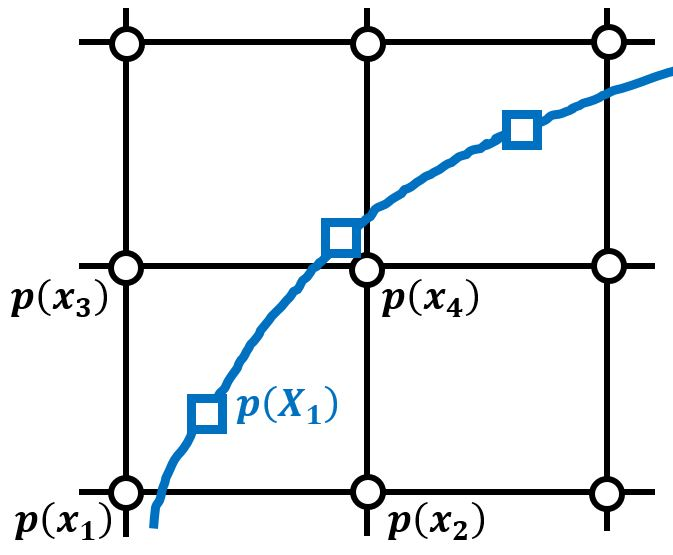
\includegraphics[width=7.00cm]{Chapter_5/figure/Chapter5_pressureMapping.jpg}
    \caption{Eulerian ($\bigcirc$) and Lagrangian ($\square$) nodes for pressure values near and on the immersed boundary.}
    \label{fig:C5_pressureMapping}
\end{figure}
%
To map this pressure information from the Eulerian nodes, $x_i$, to the Lagrangian node, $X$, we convolute the pressure field calculated from the CFD simulation with RD function of Equation \eqref{eq:C5_pressureDeltaFunction}.  By this approach we have calculated the pressure load on the structure. This is shown in Equation \eqref{eq:C5_surfacePressureCalculation}
%
\begin{subequations}
\begin{align}
    \mathcal{D}(x, X) &=
    \dfrac{-\tanh^{2}{\left (\dfrac{x - X}{\eta} \right )} + 1}{2 \eta}
    \label{eq:C5_pressureDeltaFunction}
    \\
    p(X, Y) &= \int \int p(x,y) \mathcal{D}(x, X) \mathcal{D}(y, Y) dx dy
    \label{eq:C5_surfacePressureCalculation}
\end{align}
\end{subequations}
%
By applying this pressure distribution on the solid domain and solving the equation of motion, we can calculate the displacement and the resulting velocity of the solid structure. The structure new location is used to update the RD function used for data transfer between the Eulerian and Lagrangian nodes. The cost of updating the RD functions for IB method is minuscule compared to the effort required to update the mesh in body conformal discretization approaches. The velocity of the solid domain is used for calculating the force terms required by the IB method as shown in Equation \eqref{eq:C5_immersedBoundaryForceTerm}.
%
\begin{equation}\label{eq:C5_immersedBoundaryForceTerm}
    \mathbf{f}(\mathbf{X}, t) = 
    \alpha \int_0^t \left[ \mathbf{u}(\mathbf{X}, \tau) - \mathbf{V}(\mathbf{X}, \tau) \right] d\tau + 
    \beta \left[ \mathbf{u}(\mathbf{X}, \tau) - \mathbf{V}(\mathbf{X}, \tau) \right]
\end{equation}
%
As described in Chapter \ref{ch:shapeSenwithIB}, $\mathbf{u}(\mathbf{X}, \tau)$, is the velocity of fluid calculated at the Lagrangian point $\mathbf{X}$ at time $\tau$, and $\mathbf{V}(\mathbf{X}, \tau)$ is the velocity of the solid structure at the same location and time. The later is calculated after solving the structure's equation of motion. This loop is continued until the convergence is meet or the process stoped manually. The flowchart for the fluid solid interaction using the IB method is shown in Figure \ref{fig:C5_FSIflowchart}.
%
\begin{figure}[H]
    \centering
    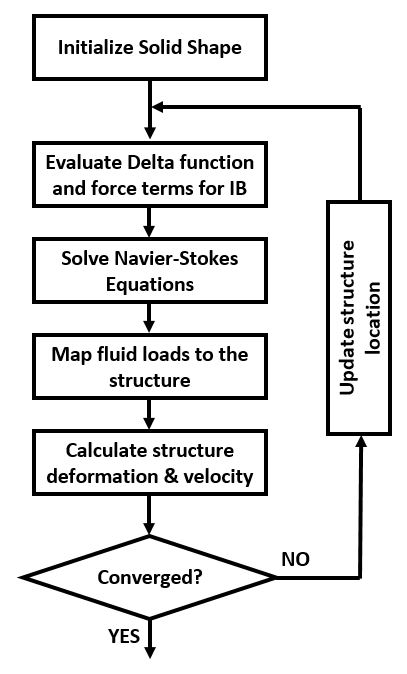
\includegraphics[width=7.00cm]{Chapter_5/figure/Chapter5_FSI_FlowChart.jpg}
    \caption{Fluid-solid interaction analysis using IB method flow chart.}
    \label{fig:C5_FSIflowchart}
\end{figure}
%
\section{Multidisciplinary Shape Sensitivity Analysis}
% =============================
The shape sensitivity analysis for the coupled multidisciplinary problem is built on the work done in Chapter \ref{ch:shapeSenwithIB}. However, in this chapter, we are also including the shape sensitivity effects on the structural side. To do so, we differentiate Equations \eqref{eq:C5_fluidGE} and \eqref{eq:C5_solidGE} alongside the kinematic and dynamic constraints of Equation \eqref{eq:C5_FSIconstraints} with respect to shape design variable, $b$. The sensitivity equations for the fluid and solid domains are shown in Equation \eqref{eq:C5_fluidSA} and \eqref{eq:C5_solidSA}, respectively.
%
\begin{subequations}\label{eq:C5_fluidSA}
\begin{align}
	&\rho^f \frac{\partial}{\partial t} \left( \frac{\partial \mathbf{u}^f}{\partial b} \right) + 
	\rho^f \frac{\partial \mathbf{u}^f}{\partial b} \cdot \nabla \mathbf{u}^f +
	\rho^f \mathbf{u}^f \cdot \nabla \left( \frac{\partial \mathbf{u}^f}{\partial b} \right) = 
	\nabla \cdot \left( \frac{\partial \mathbf{\sigma}^f}{\partial b} \right) +
	\rho^f \frac{\partial \mathbf{f}^f}{\partial b}
	\\
	&\nabla \cdot \left( \frac{\partial \mathbf{u}^f}{\partial b} \right) = 0
	\\
	&\frac{\partial \mathbf{\sigma}^f}{\partial b} = 
	\mu \left[ \nabla \left( \frac{\partial \mathbf{u}^f}{\partial b} \right) + 
	           \nabla \left( \frac{\partial \mathbf{u}^f}{\partial b} \right)^T \right] - 
	\frac{\partial p^f}{\partial b} \mathbf{I}
\end{align}
\end{subequations}
%
\begin{subequations}\label{eq:C5_solidSA}
\begin{align}
	\rho^s \frac{\partial \dot{\mathbf{u}}^s}{\partial b} &= 
	\nabla \cdot \left( \frac{\partial \sigma^s}{\partial b} \right) + 
	\frac{\partial \mathbf{f}^s}{\partial b}
	\\
	\frac{\partial \mathbf{\epsilon^s}}{\partial b} &=
	\frac{1}{2}
	\left[ \nabla \frac{\partial \mathbf{d}^s}{\partial b} + \nabla \left( \frac{\partial \mathbf{d}^s}{\partial b} \right)^T \right]
	\\
	\frac{\partial \mathbf{\sigma}^s}{\partial b} &= 
	\frac{\partial \mathbf{C}}{\partial b} : \mathbf{\epsilon}^s + 
	\mathbf{C} : \frac{\partial \mathbf{\epsilon}^s}{\partial b}
\end{align}
\end{subequations}
%
%
%\begin{subequations}\label{eq:C5_FSIconstraintsSA}
%\begin{align}
%	\frac{\partial \mathbf{u}^s}{\partial b} - 
%	\frac{\partial \mathbf{u}^f}{\partial b} &= 0
%	\\
%	\frac{\partial \mathbf{\sigma}^s}{\partial b} \cdot \mathbf{n} - 
%	\frac{\partial \mathbf{\sigma}^f}{\partial b} \cdot \mathbf{n} &= 0
%\end{align}
%\end{subequations}
\begin{subequations}\label{eq:C5_FSIconstraintsSA}
\begin{align}
	\frac{D \mathbf{u}^s}{D b} - 
	\frac{D \mathbf{u}^f}{D b} &= 0
	\\
	\frac{D \mathbf{\sigma}^s}{D b} \cdot \mathbf{n} - 
	\frac{D \mathbf{\sigma}^f}{D b} \cdot \mathbf{n} &= 0
\end{align}
\end{subequations}
%
The derivatives of the interface conditions of Equation \eqref{eq:C5_FSIconstraintsSA} are written and simplified using the chaine rule. Here we show the process for the Dirichlet boundary condition. The same approach can be done for the Neumann boudaries as well.
%
\begin{gather*}
	\overbrace{	
	\left(
	\frac{\partial \mathbf{u}^s}{\partial b} +
	\frac{\partial \mathbf{u}^s}{\partial \mathbf{x}^s} \frac{\partial \mathbf{x}^s}{\partial b} +
	\frac{\partial \mathbf{u}^s}{\partial \mathbf{x}^f} \frac{\partial \mathbf{x}^f}{\partial b}
	\right)
	}^{\dfrac{D \mathbf{u}^s}{D b}} -
	\overbrace{
	\left(
	\frac{\partial \mathbf{u}^f}{\partial b} +
	\frac{\partial \mathbf{u}^f}{\partial \mathbf{x}^s} \frac{\partial \mathbf{x}^s}{\partial b} +
	\frac{\partial \mathbf{u}^f}{\partial \mathbf{x}^f} \frac{\partial \mathbf{x}^f}{\partial b}
	\right)
	}^{\dfrac{D \mathbf{u}^f}{D b}} = 0 \Longrightarrow
	\\
	\left(
	\frac{\partial \mathbf{u}^s}{\partial b} - \frac{\partial \mathbf{u}^f}{\partial b}
	\right) +
	\left(
	\frac{\partial \mathbf{u}^s}{\partial \mathbf{x}^s} - 
	\frac{\partial \mathbf{u}^f}{\partial \mathbf{x}^s}
	\right) \frac{\partial \mathbf{x}^s}{\partial b} +
	\left(
	\frac{\partial \mathbf{u}^s}{\partial \mathbf{x}^f} - 
	\frac{\partial \mathbf{u}^f}{\partial \mathbf{x}^f}
	\right) \frac{\partial \mathbf{x}^f}{\partial b} = 
	0 \Longrightarrow
	\\
	\left(
	\frac{\partial \mathbf{u}^s}{\partial b} - \frac{\partial \mathbf{u}^f}{\partial b}
	\right) +
	\frac{\partial }{\partial \mathbf{x}^s}
	\underbrace{	
	\left(
	\mathbf{u}^s - \mathbf{u}^f
	\right)
	}_{=\mathbf{0}} \frac{\partial \mathbf{x}^s}{\partial b} +
	\frac{\partial }{\partial \mathbf{x}^f}
	\underbrace{	
	\left(
	\mathbf{u}^s - \mathbf{u}^f
	\right)
	}_{=\mathbf{0}} \frac{\partial \mathbf{x}^f}{\partial b} = 
	0 \Longrightarrow
	\\
	\frac{\partial \mathbf{u}^s}{\partial b} - 
	\frac{\partial \mathbf{u}^f}{\partial b} = 0
\end{gather*}
%
Sensitivity of solid shape movement is represented in the derivative of the forcing function, $\mathbf{f}^f$ in Equation \eqref{eq:C5_fluidSA}. In particular the geometric sensitivity of the solid boundary is added to the governing equations through the derivative of the regulirized delta function in Equation \eqref{eq:C5_fluidSA}. However, as discussed in Chapter \ref{ch:sensitivityAnalysis}, the geometric sensitivity does not propagate inside the domain since the fluid mesh does not move.

To solve the sensitivity equations we need to obtain the solution of the governing equation ($\mathbf{u}^f$, $\mathbf{\epsilon^s}$). Therefore, we are proposing to use the flowchart of Figure \ref{fig:C5_SAflowchart} for the coupled multidisciplinary sensitivity analysis. The sensitivity calculation process starts by solving the Navier-Stokes equation and mapping the pressure to the structural domain to calculate the deformation in the structural domain. The solution of the Navier-Stokes and Elasticity equations are then fed to the sensitivity solver to calculate the sensitivity response. This loop is continued until a convergence for the governing equations is reached or the process is stopped manually. 
%
\begin{figure}[H]
    \centering
    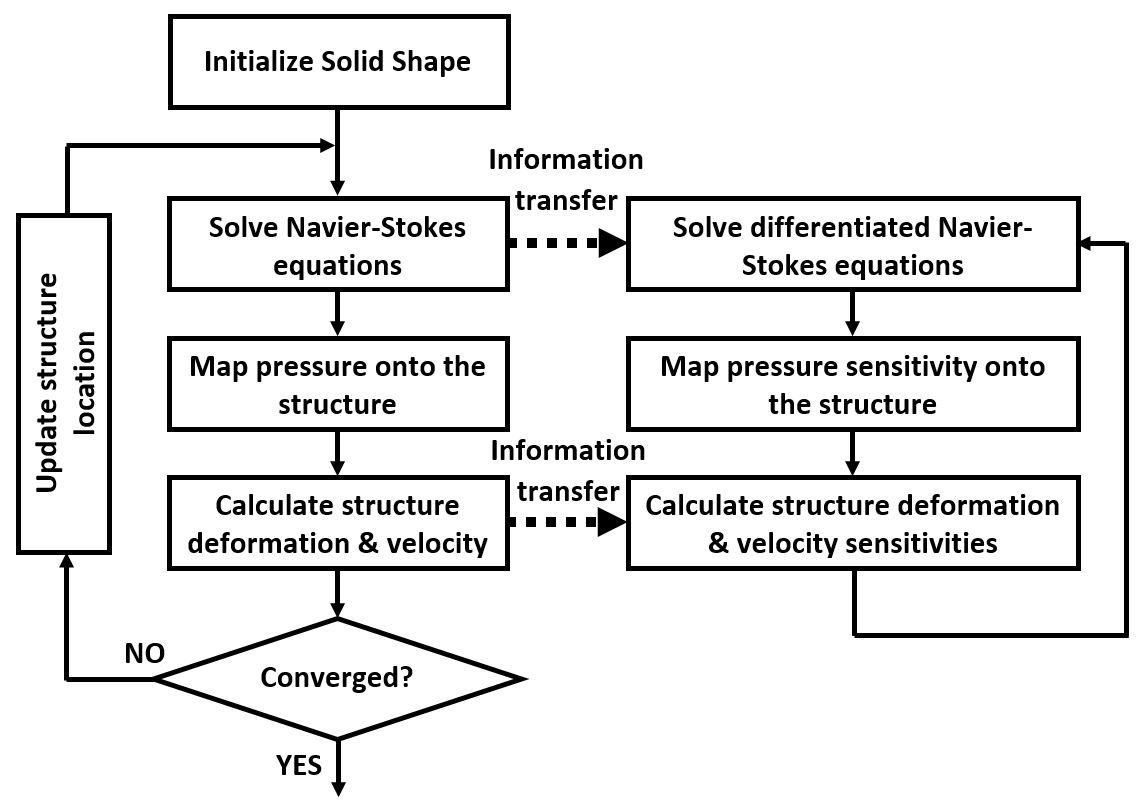
\includegraphics[width=14.00cm]{Chapter_5/figure/couple_SA_flowchart.jpg}
    \caption{Coupled multidisciplinary sensitivity analysis flowchart. The loop represents time marching for solution convergence.}
    \label{fig:C5_SAflowchart}
\end{figure}
%
\section{Demonstration Cases}
\subsection{Vortex Induced Vibration}
Vortex Induced Vibrations (VIV) are motions of solid structures immersed in fluid that are caused by the irregularities in the flow. VIV of structures are of practical interest to many fields of engineering. For example, they can cause vibration and noise in heat exchanger tubes and an aircraft wing. The practical significance of VIV has led to various studies discussed in the literature\cite{williamson2004vortex}. In this demonstration problem, we are interested in the forced oscillations of an elastically mounted, rigid cylinder for different values of the Reynolds number. The physical problem is shown in Figure \ref{fig:C5_cylinderShape}. The boundary conditions are selected as constant velocity at inlet, free slip boundary conditions on top and bottom walls, and outflow boundary condition at the outlet.
%
\begin{figure}[H]
    \centering
    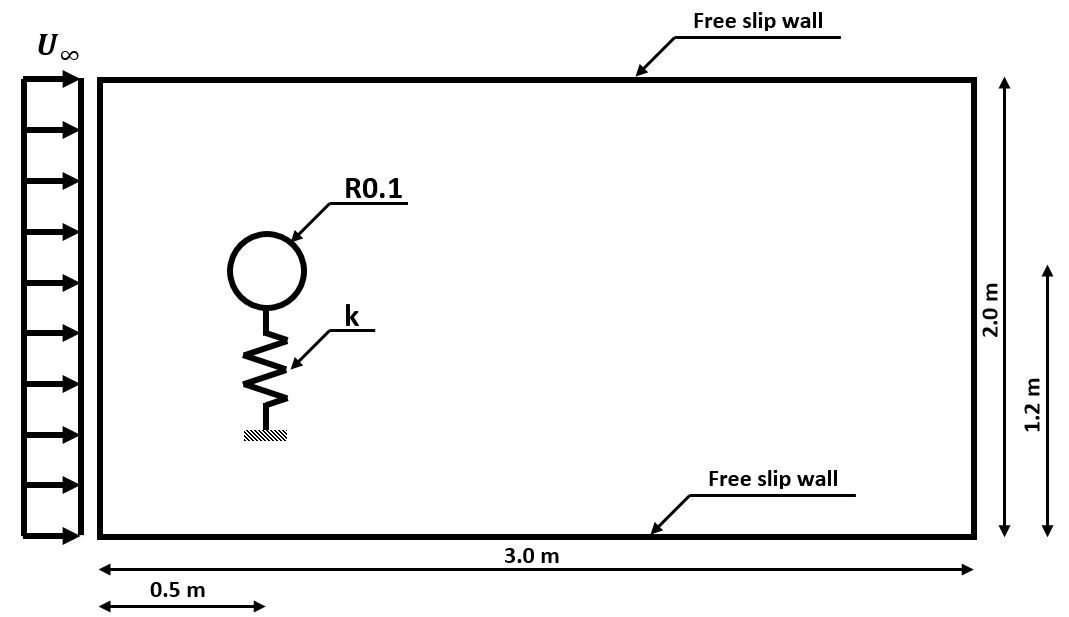
\includegraphics[width=9.00cm]{Chapter_5/figure/VIV_domain_shape.jpg}
    \caption{Physical domain for the vortex induced vibration problem.}
    \label{fig:C5_cylinderShape}
\end{figure}
%
The rigid cylinder has the radius $R$ and is mounted on an elastic structure with stiffness $k$. The free steam velocity is selected as $U_\infty$. To verify the solver and FSI coupling, we are going to calculate the shedding frequency of the cylinder first. Vortex shedding is an oscillating flow that takes place when fluid passes a bluff body at certain velocities. The vortices that are generated on the aft of the body start to detach periodically from either side of the body. The frequency at which the vortex shedding takes place is described using the dimensionless Strouhal number. The Strouhal number is defined as shown in Equation \eqref{eq:C5_strouhalNumber}.
%
\begin{equation}\label{eq:C5_strouhalNumber}
	St = \frac{fL}{U}
\end{equation}
%
where $f$ is the frequency of the vortex shedding; $L$ is the characteristic length; and $U$ is the flow velocity. The Strouhal number of a stationary circular cylinder is a function of Reynolds number \cite{chen1987flow} as shown in Figure \ref{fig:C5_strouhalVSreynoldsNumber}\cite{jendrzejczyk1985fluid}.
%
\begin{figure}[H]
    \centering
    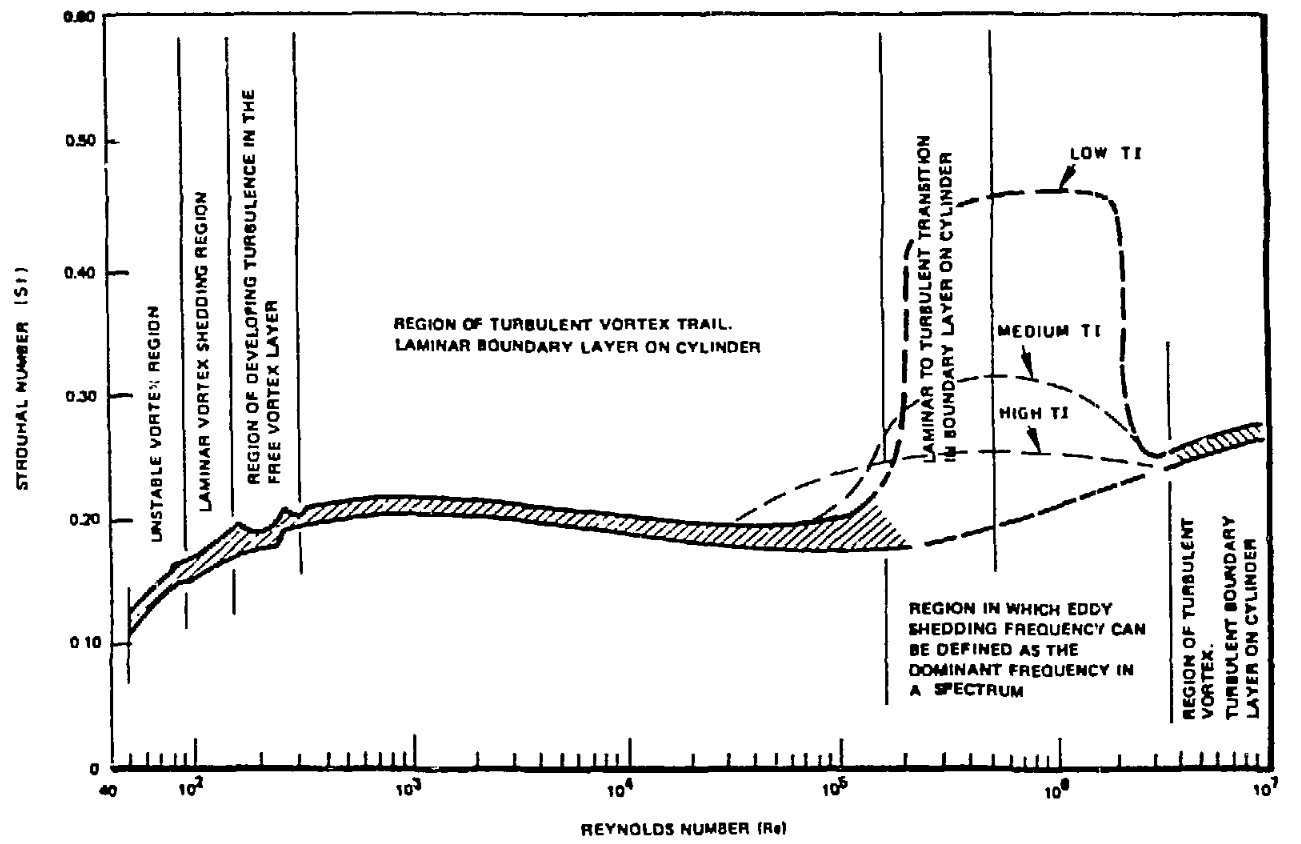
\includegraphics[width=10.00cm]{Chapter_5/figure/StrouhalVsReynodsl.png}
    \caption{Strouhal number for a single cylinder.}
    \label{fig:C5_strouhalVSreynoldsNumber}
\end{figure}
%
To verify the simulation code developed for the IB simulation, we verified the shedding frequency of the circular cylinder in the cross-flow. The domain length and height are selected as $3 m$ and $2 m$, respectively, as shown in Figure \ref{fig:C5_cylinderShape}. The cylinder radius is selected as $0.1 m$ and is located $0.5 m$ from the left wall and $1.2 m$ from the bottom wall. The asymmetric shape of the computational domain helps the shedding initiation. The domain is discretized using $3000$ cells in the $x$ direction and $2000$ in the $y$. The cylinder is defined using $50$ Lagrangian nodes. The $p$ value in the delta function definition is selected as $0.5$. It should be noted that to verify the shedding frequency the cylinder is fixed in its place. We compared the Strouhal number calculated from the IB code with the results \cite{mittal2001control} for two different Reynolds numbers. The shedding frequency is calculated by saving the time history of drag force on the cylinder and performing frequency analysis on this data. We used the power spectral density function to look at the most dominant frequencies. The comparison between these results is shown in Table \ref{table:C5_strouhalVerification}.
%
\begin{table}[H]
\centering
\begin{tabular}{c | c | c}
     Reynolds number & St (current IB) & St (Literature \cite{jendrzejczyk1985fluid} and \cite{mittal2001control}) \\ \hline \hline
     100 & 0.171 & 0.168 \\ \hline
     500 & 0.194 & 0.200 \\
\end{tabular}
\caption{Comparison between the shedding frequency calcualted using IB method and results from the literature.}
\label{table:C5_strouhalVerification}
\end{table}
%
The effect of the number of Lagrangian points on the shedding frequency is shown in Figure \ref{fig:C5_numberOfLagrangianOnSheddingFreq} for the two Reynolds numbers of 100 and 500. As shown here, the number of Lagrangian points does not affect the vortex shedding frequency.
%
\begin{figure}[H]
    \centering
    \subfigure[$Re = 100$]
    {
    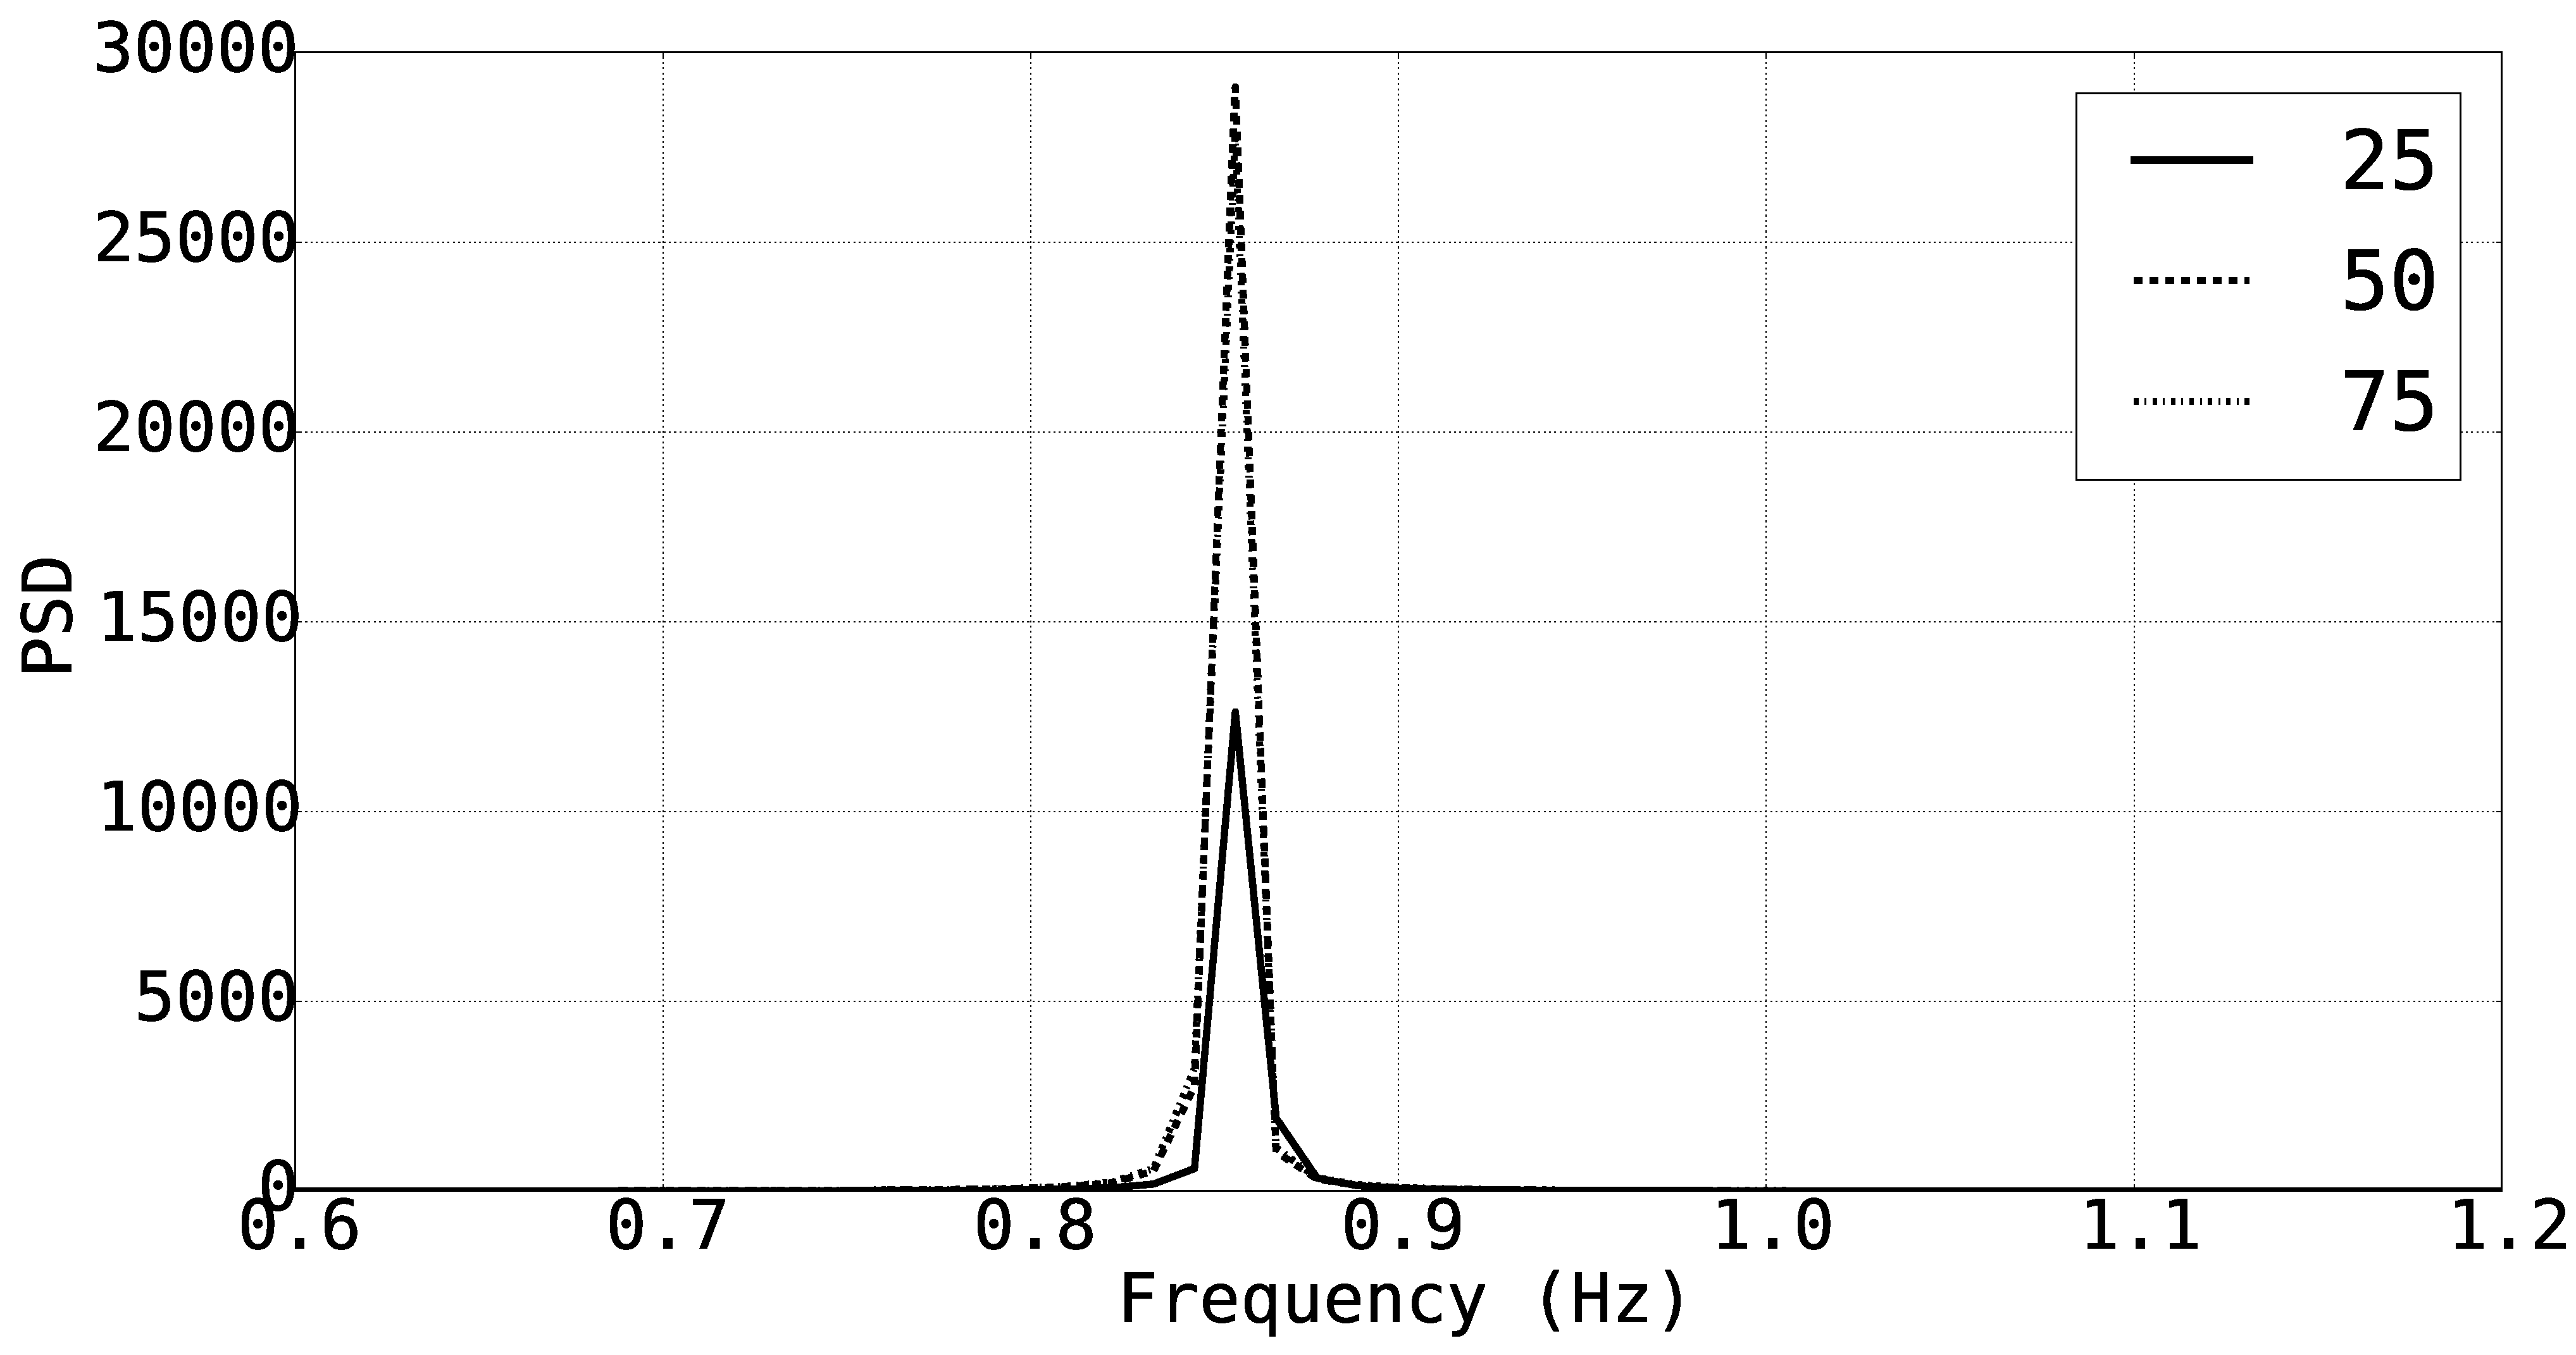
\includegraphics[width=9.0cm]{Chapter_5/figure/PSD_Re100.eps}
    }
    \quad
    \subfigure[$Re = 500$]
    {
    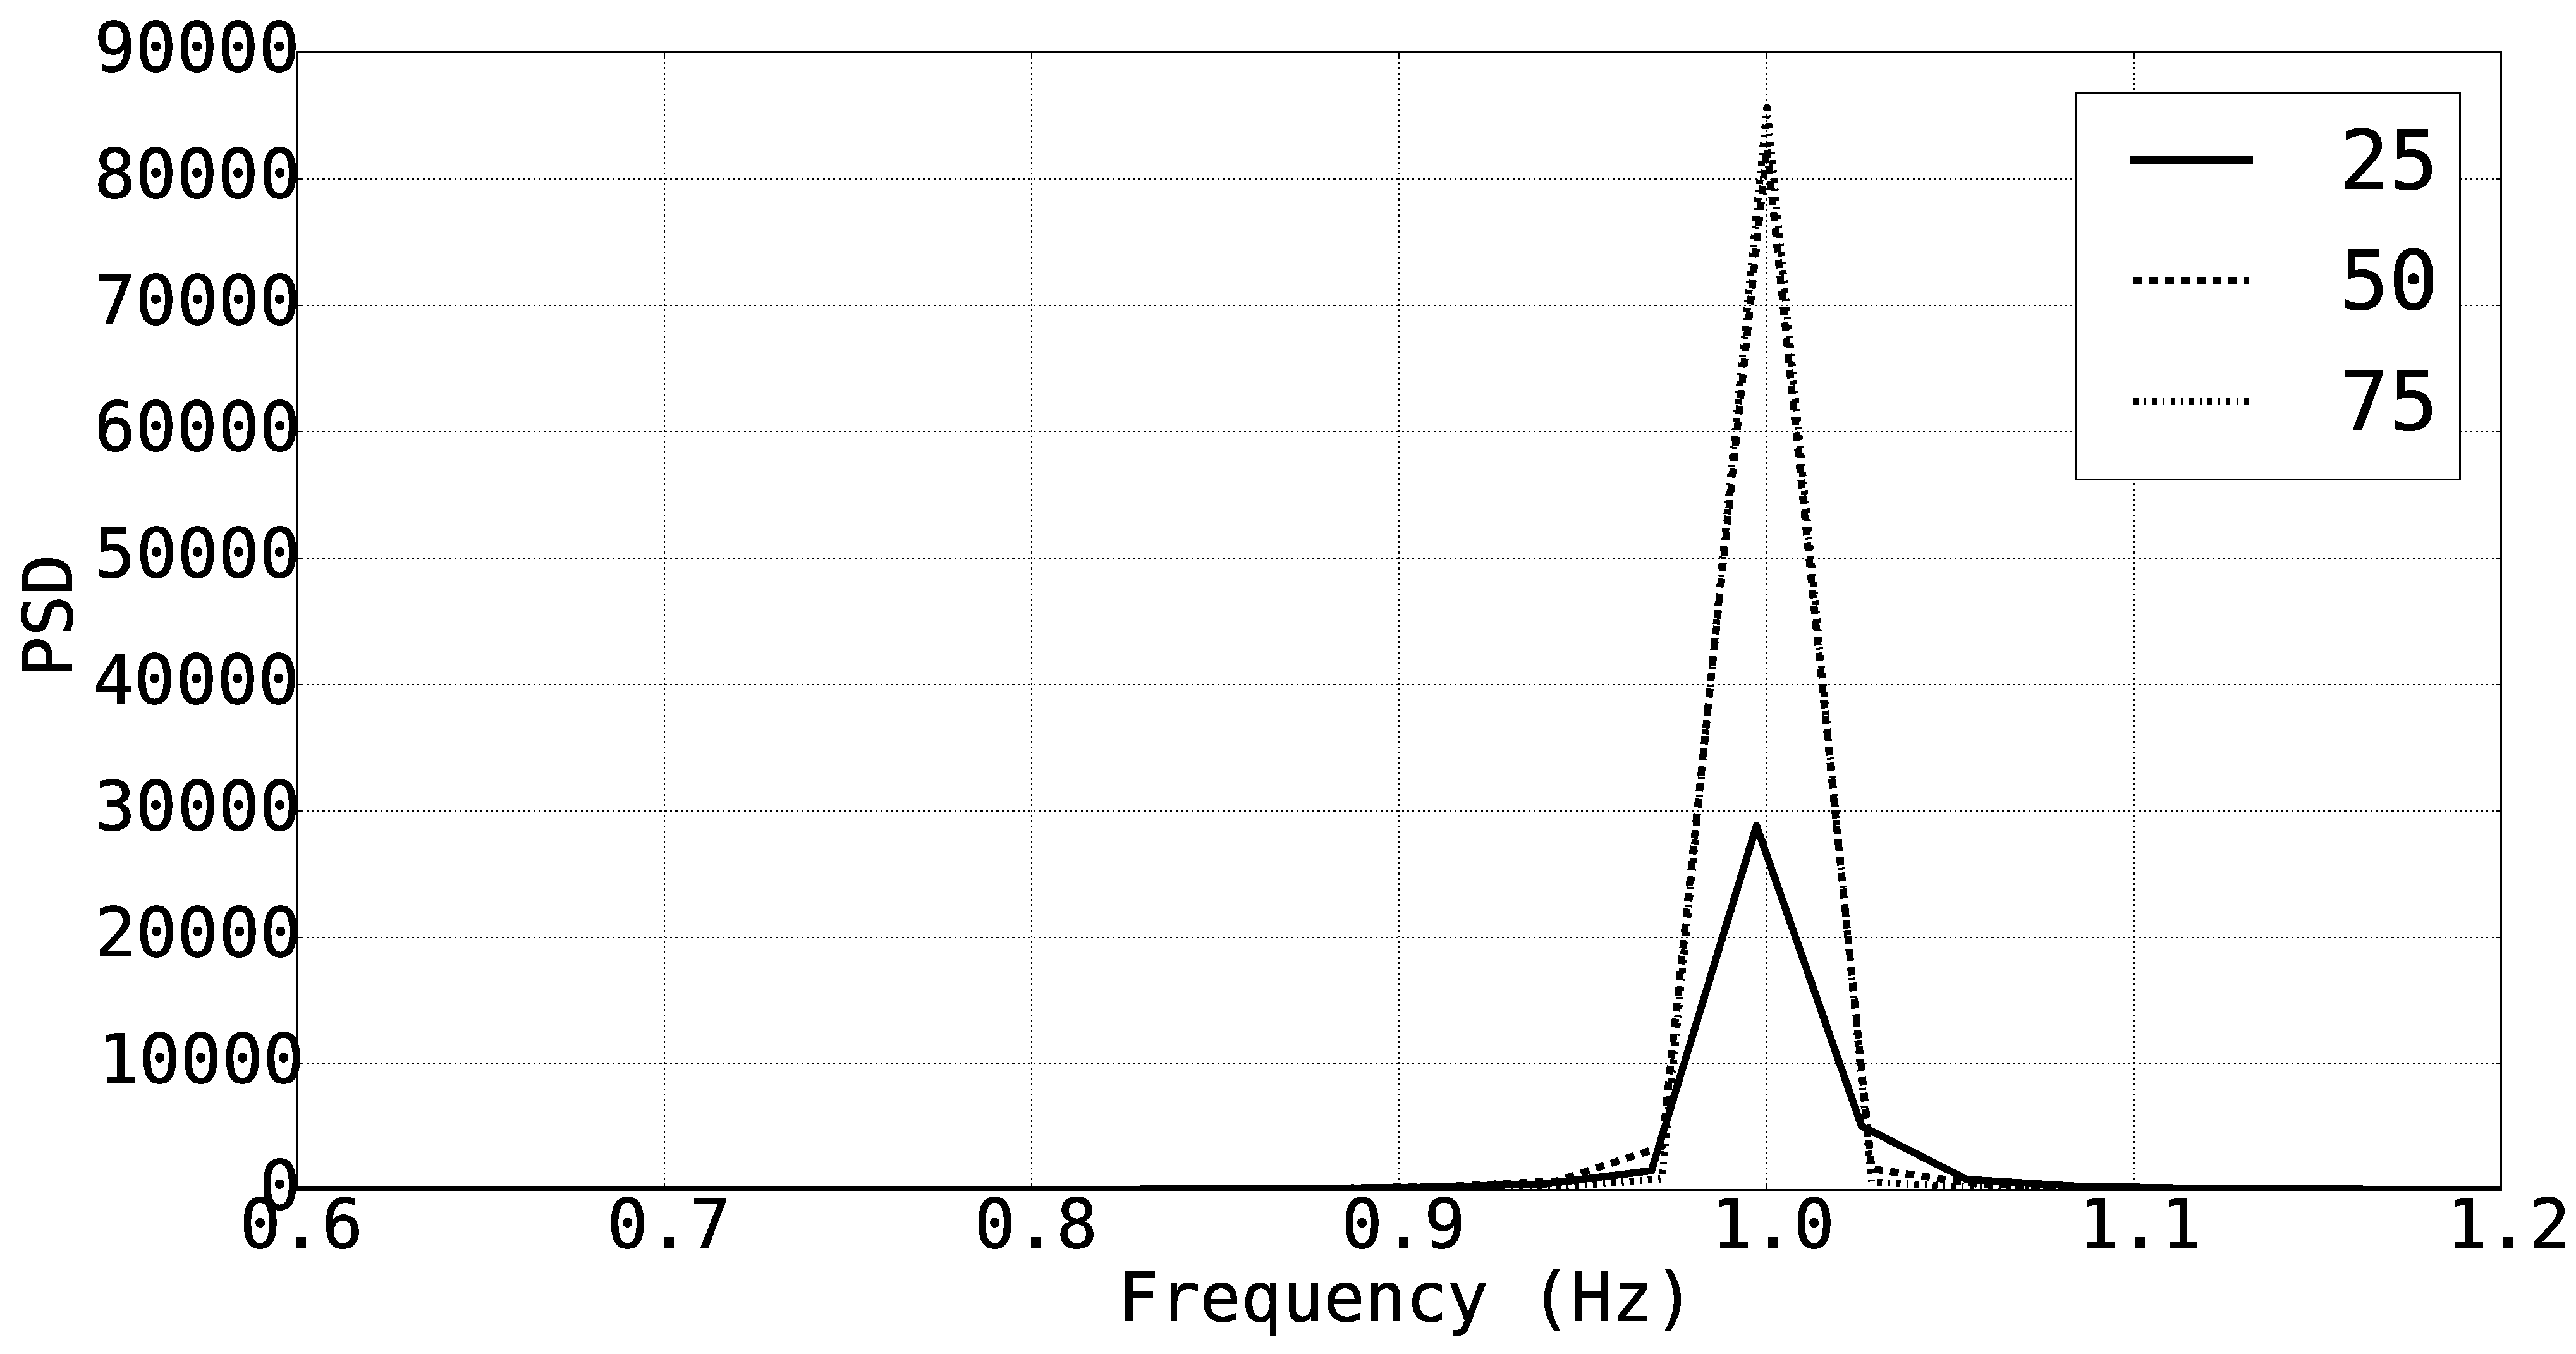
\includegraphics[width=9.0cm]{Chapter_5/figure/PSD_Re500.eps}
    }
    \caption{Number of Lagrangian points effect on the shedding frequency.}
    \label{fig:C5_numberOfLagrangianOnSheddingFreq}
\end{figure}
%
After verifying the shedding frequency of IB solver, we attach the elastic structure to the cylinder and let the system vibrate due to aerodynamic loads. The equation of motion for this cylinder is shown in Equation \eqref{eq:C5_cylinderEquationOfMotion}.
%
\begin{equation}\label{eq:C5_cylinderEquationOfMotion}
	m \ddot{y} + k y = f(y, \dot{y}, t; R)
\end{equation}
%
where $y$ is the cylinder location; $m$ is the cylinder mass; $k$ is elastic structure stiffness; and $f(y, \dot{y}, t; R)$ is the aerodynamic load. It should be noted that the load is an explicit function of cylinder location, velocity, and time, while an implicit function of cylinder radius. This requires an unsteady treatment of the FSI problem by coupling Equation \eqref{eq:C5_fluidGE} and \eqref{eq:C5_cylinderEquationOfMotion}.

At each time step, the NS equations are solved and the pressure values at the Lagrangian nodes are calculated using the regularized Delta function. These pressure values are then integrated over the cylinder surface to calculate the force value on the right-hand-side of Equation \eqref{eq:C5_cylinderEquationOfMotion}. To solve for the structure displacement and velocity, Equation \eqref{eq:C5_cylinderEquationOfMotion} is written in the state-space form as shown in Equation \eqref{eq:C5_cylinderEquationOfMotionStateSpace}. This equation is then integrated in time alongside the NS equations using Adams-bashforth method. The initial condition for the structure is selected as zero displacement and velocity at $t = 0$.
%
\begin{equation}\label{eq:C5_cylinderEquationOfMotionStateSpace}
	\begin{bmatrix}
	\dot{y} \\
	\ddot{y}
	\end{bmatrix} = 
	\begin{bmatrix}
	0 & 1 \\
	-\dfrac{k}{m} & 0
	\end{bmatrix}
	\begin{bmatrix}
	y \\
	\dot{y}
	\end{bmatrix} + 
	\begin{bmatrix}
	0 \\
	f(y, \dot{y}, t; R)
	\end{bmatrix}
\end{equation}
%
where the load, $f(y, \dot{y}, t; R)$, is calculated  as shown in Equation \eqref{eq:C5_loadOnCylidner}.
%
\begin{equation}\label{eq:C5_loadOnCylidner}
	f = \oint \left( \int \int p(x, y) \mathcal{D}(x - X_s) \mathcal{D}(y - Y_s) dx dy\right) ds
\end{equation}
%
In Equation \eqref{eq:C5_loadOnCylidner}, $p(x, y)$ is the pressure calculated from the CFD solution; $\mathcal{D}$ is the regularized delta function; and $ds$ represents the infinitesimal element on the cylinder surface.

For the coupled FSI sensitivity analysis, we looked at the vortex induced vibration of the cylinder at two different Reynolds numbers. The sensitivity of the displacement to the radius of the cylinder is calculated and verified with the complex step results. The sensitivity equation for the fluid domain is derived in Chapter \ref{ch:shapeSenwithIB}, by solving it, we have the sensitivity of pressure field on the surface of the cylinder. The sensitivity equation for the structure is derived by differentiating Equation \eqref{eq:C5_cylinderEquationOfMotionStateSpace} as shown in Equation \eqref{eq:C5_cylinderEquationOfMotionSAStateSpace}.
%
\begin{equation}\label{eq:C5_cylinderEquationOfMotionSAStateSpace}
	\begin{bmatrix}
	\dot{y'} \\
	\ddot{y'}
	\end{bmatrix} = 
	\begin{bmatrix}
	0 & 1 \\
	-\dfrac{k}{m} & 0
	\end{bmatrix}
	\begin{bmatrix}
	y' \\
	\dot{y'}
	\end{bmatrix} + 
	\begin{bmatrix}
	0 \\
	f'(y, \dot{y}, t; R)
	\end{bmatrix}
\end{equation}
%
here, $()'$, represents the derivative with respect to the design variable. As can be seen, the same solver used for solving Equation \eqref{eq:C5_cylinderEquationOfMotionStateSpace} is utilized for solving Equation \eqref{eq:C5_cylinderEquationOfMotionSAStateSpace}. The only difference between the two is the load used for evaluating the right-hand-side of Equation \eqref{eq:C5_cylinderEquationOfMotionSAStateSpace}.

For this problem, the stiffness of the elastic structure, $k$, is selected as 1 N/m and the cylinder mass is chosen as 1 kg. The time history of cylinder displacement in the first 25 seconds of its motion is shown in Figure \ref{fig:C5_cylinderDisplacement}. As can be seen here, the cylinder starts from the initial position at $y=1.2$, and after a short transient region, starts oscillating at an almost constant amplitude as shown in Figure \ref{fig:C5_cylinderDisplacement}.
%
\begin{figure}[H]
    \centering
    \subfigure[$Re = 100$]
    {
    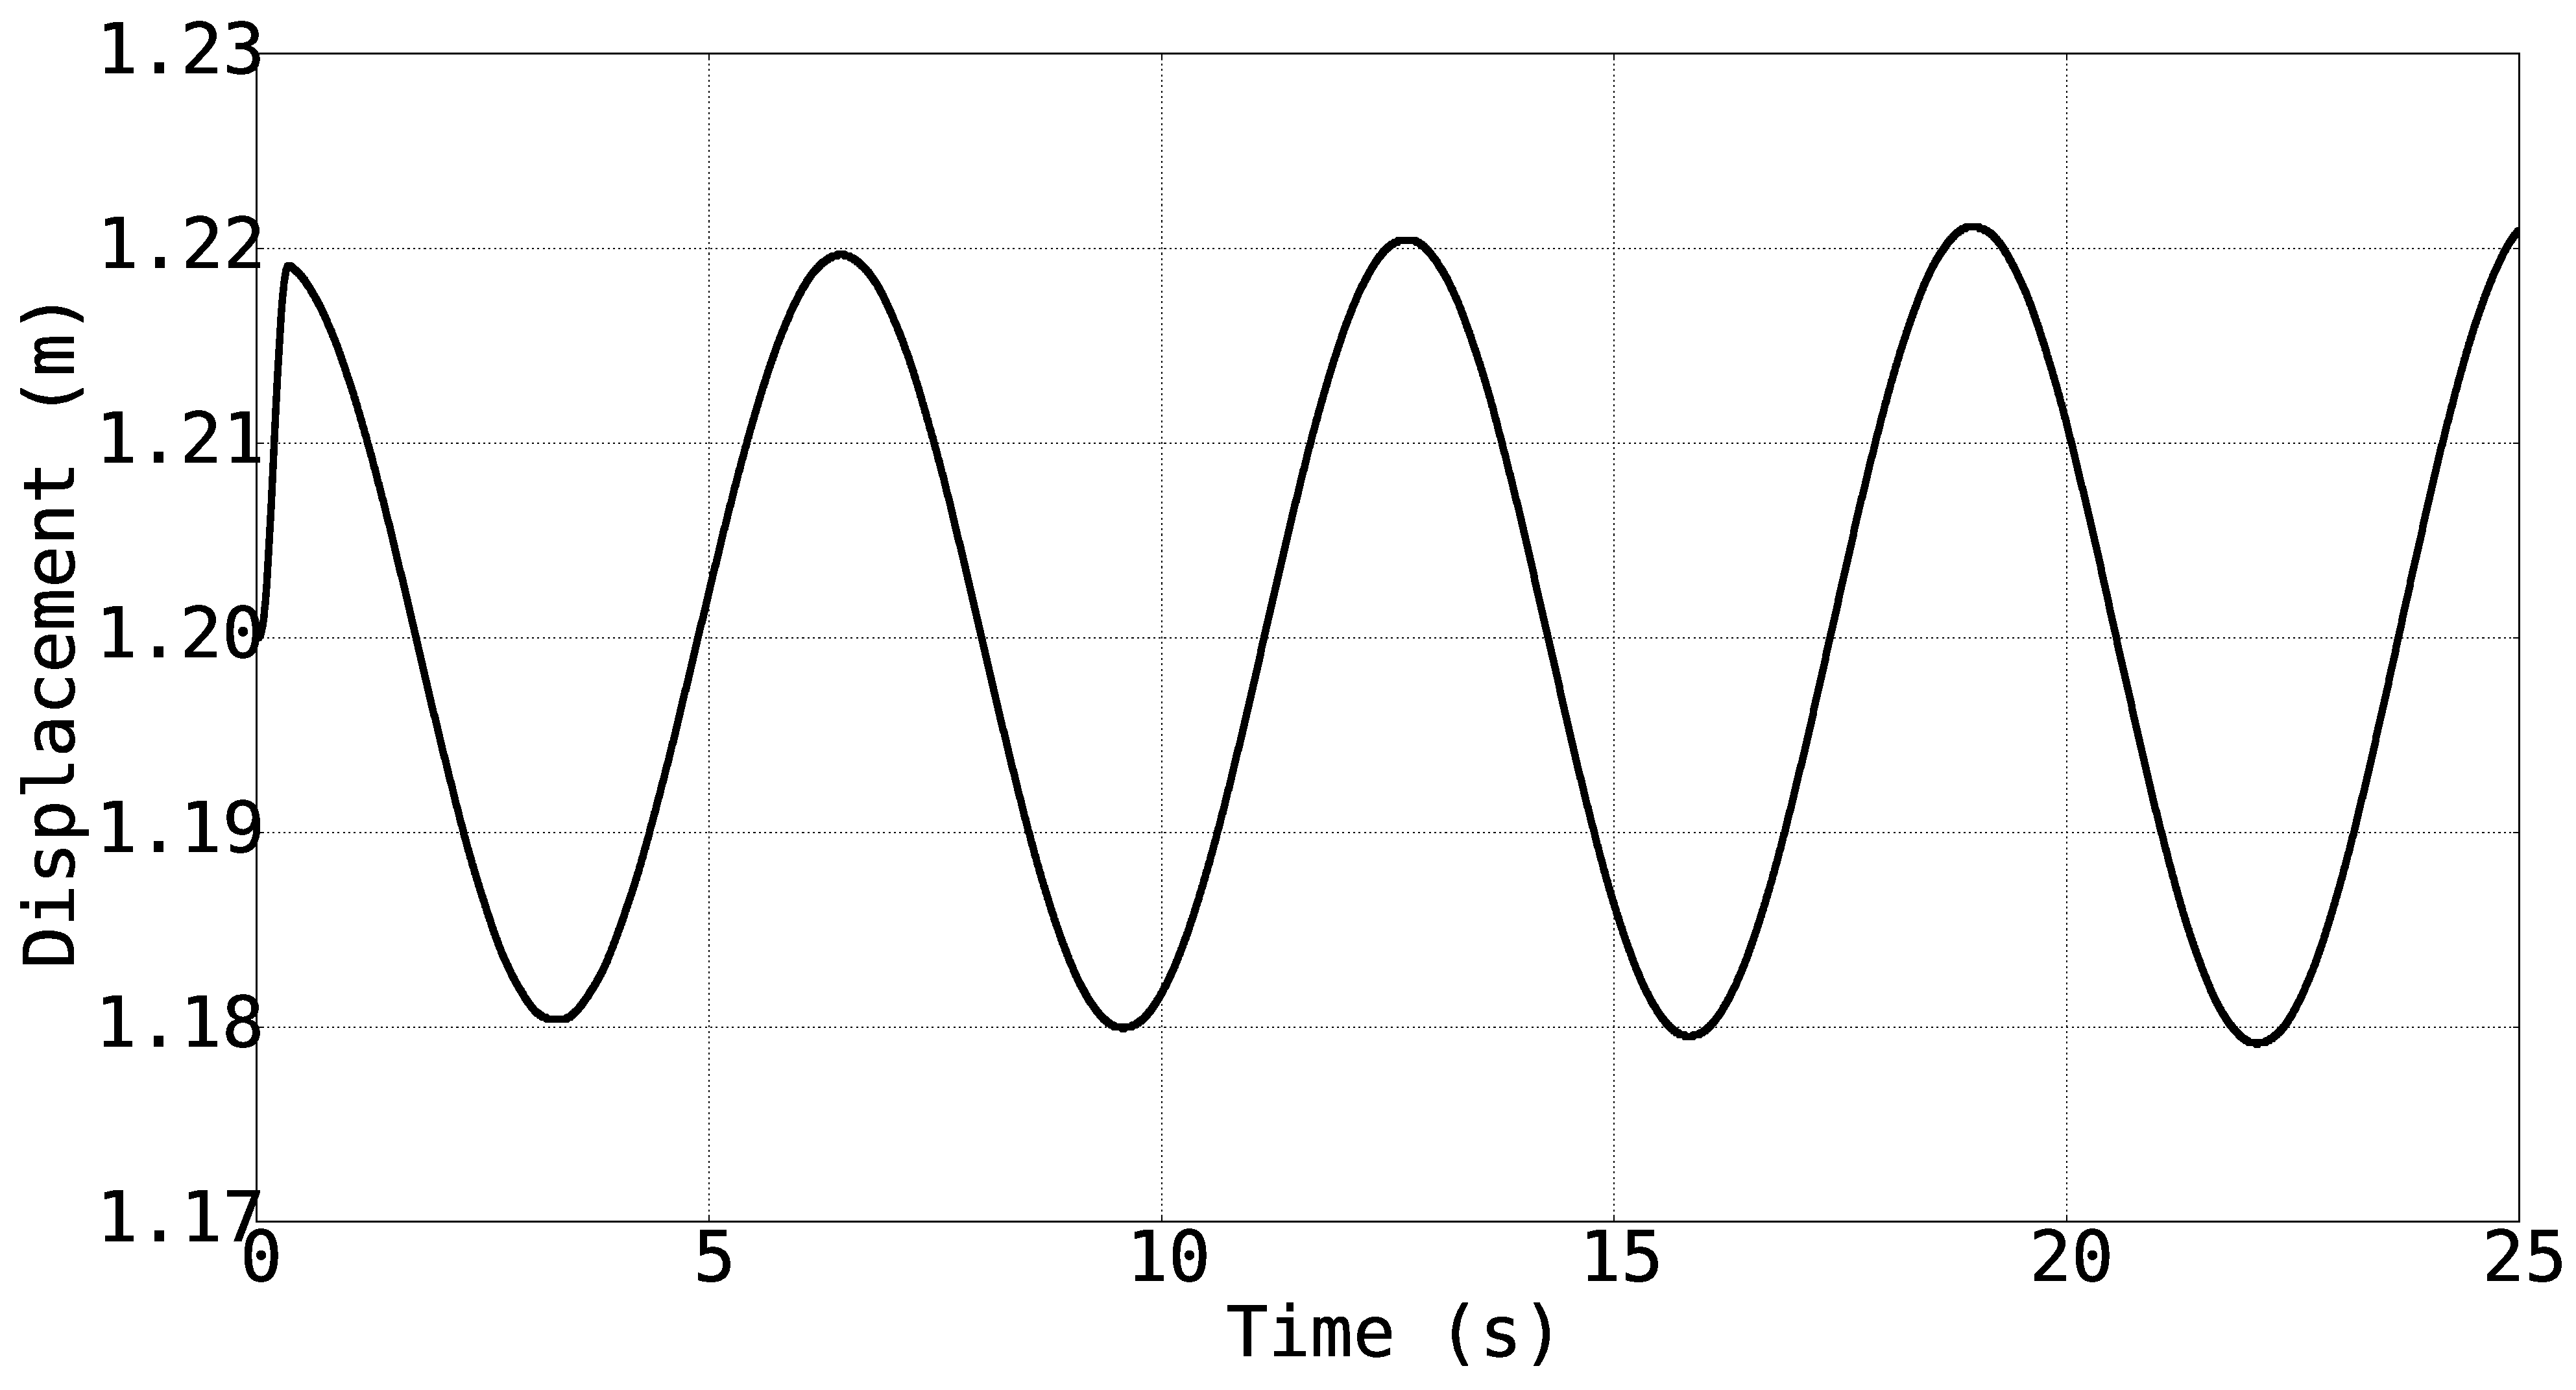
\includegraphics[width=9.0cm]{Chapter_5/figure/cylinder_Re100_Displacement.eps}
    }
    \quad
    \subfigure[$Re = 500$]
    {
    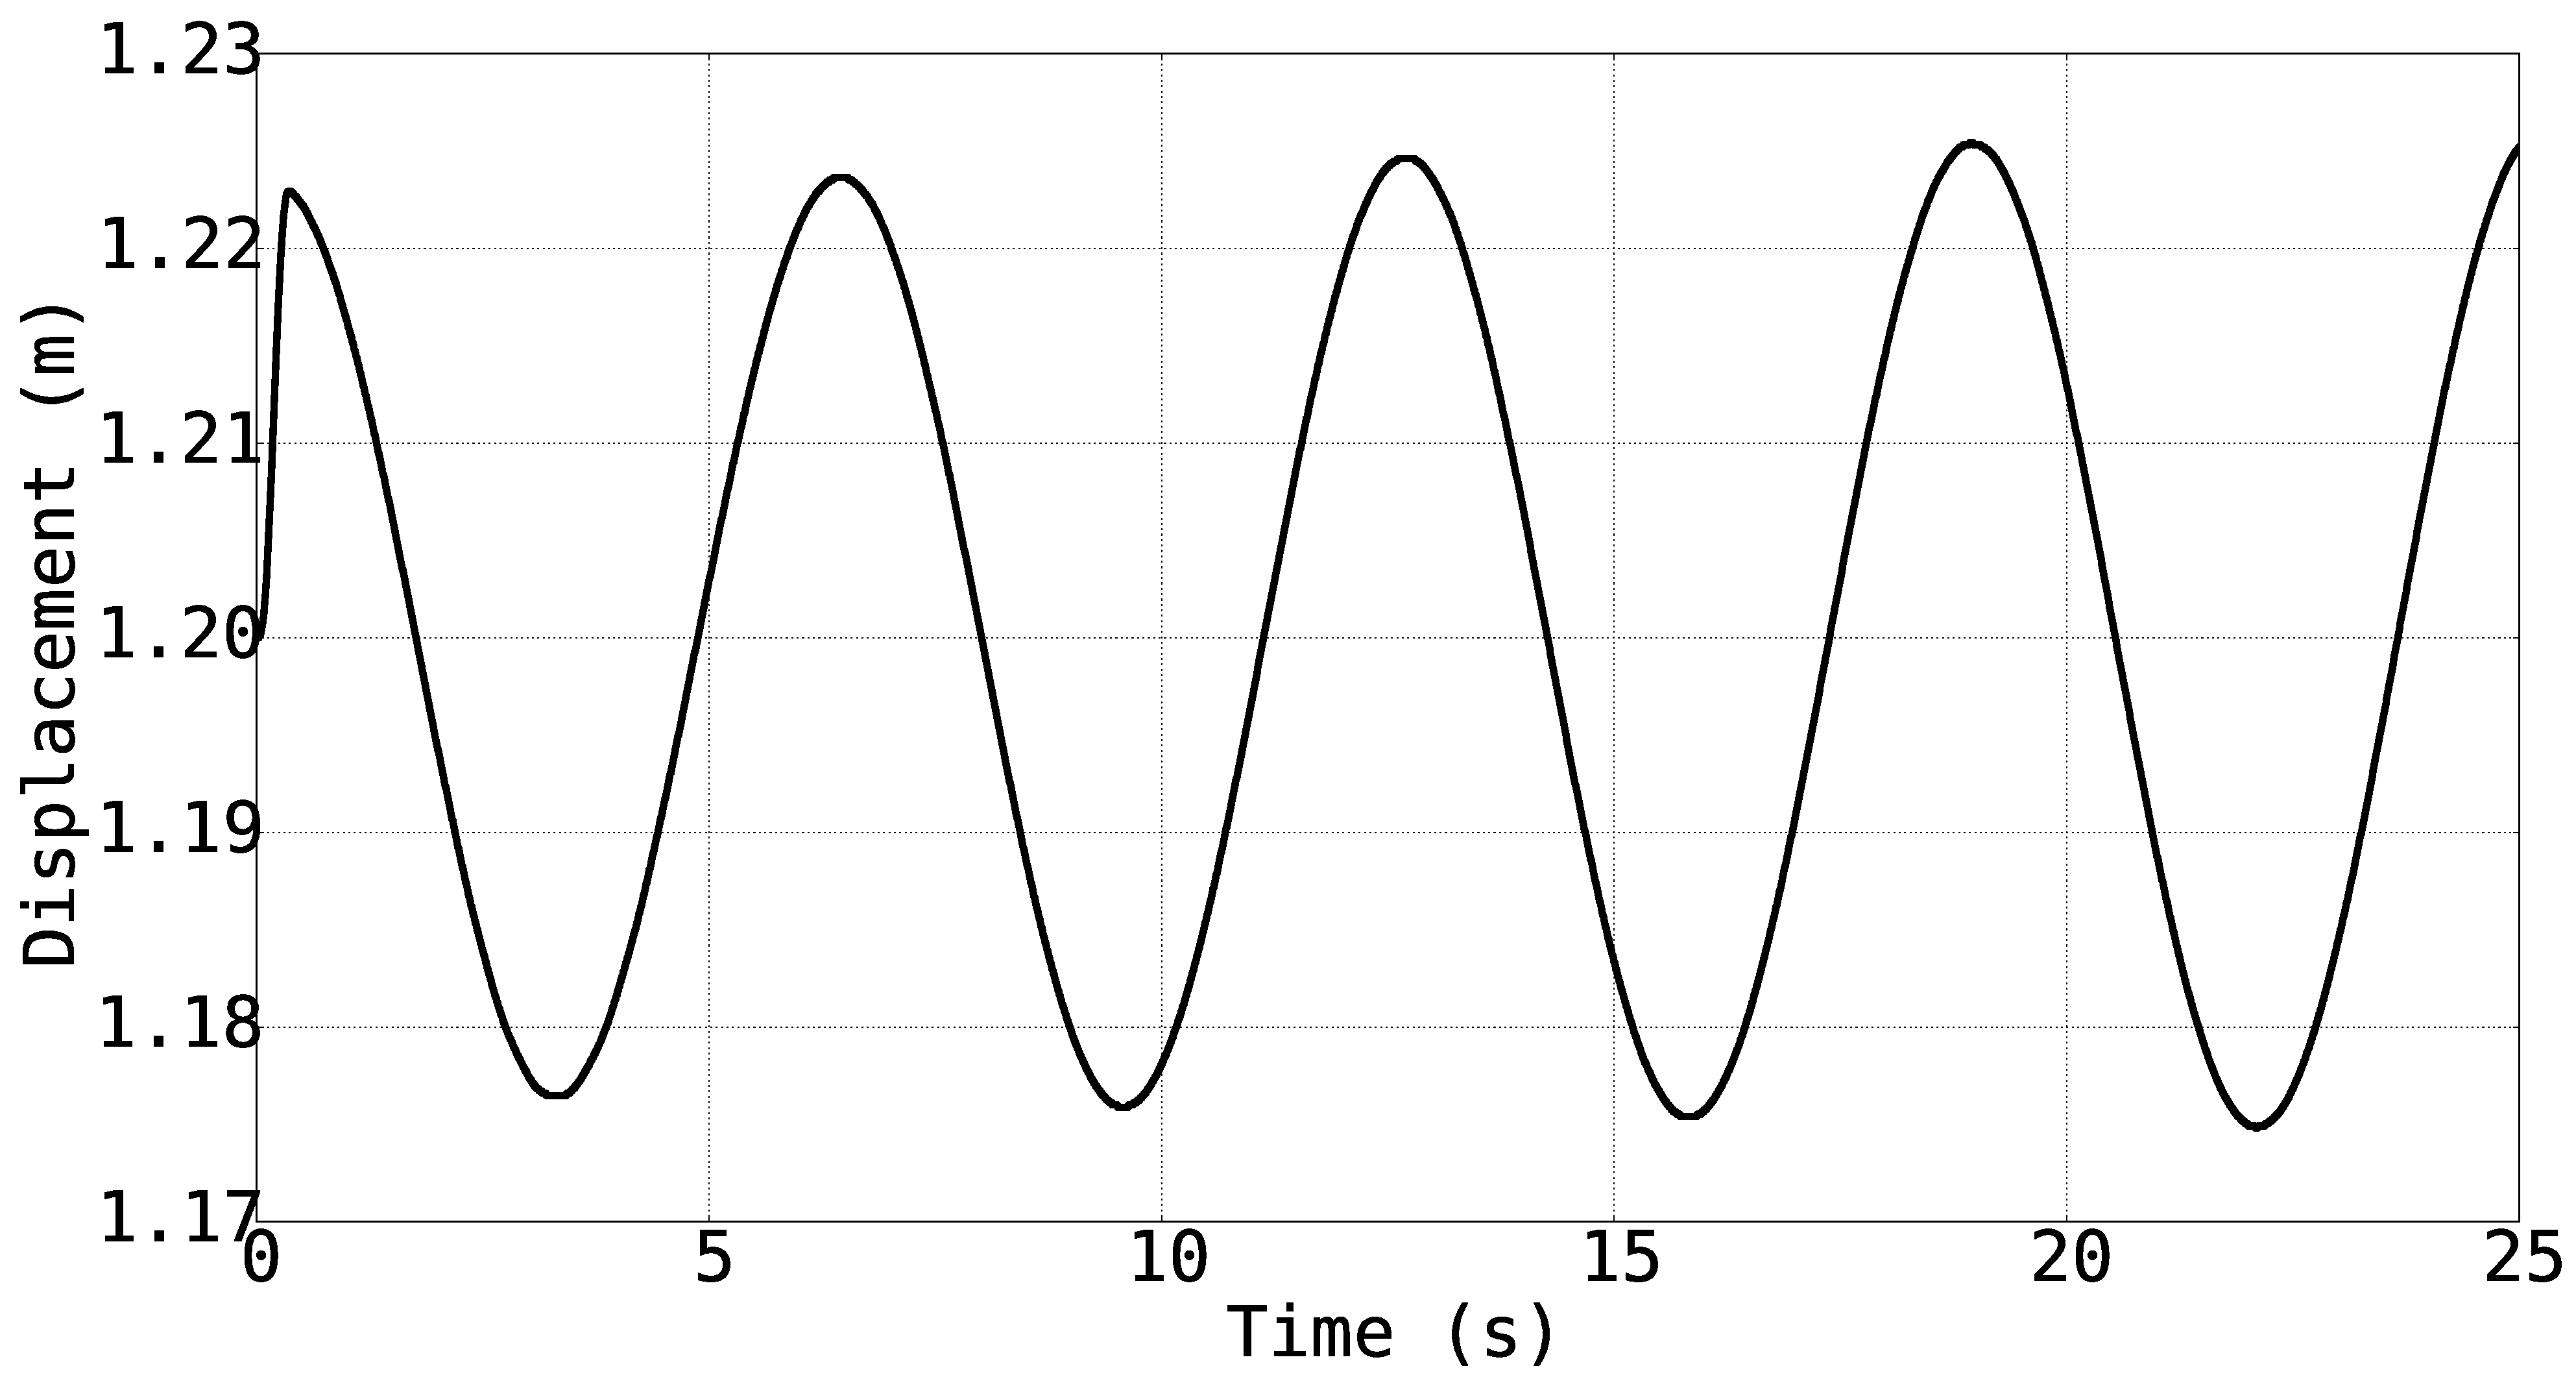
\includegraphics[width=9.0cm]{Chapter_5/figure/cylinder_Re500_Displacement.eps}
    }
    \caption{Time history of cylinder center displacement.}
    \label{fig:C5_cylinderDisplacement}
\end{figure}
%
Figure \ref{fig:C5_cylinderFSIvelocity} shows the u-velocity contour around the elastically mounted cylinder at different times. As can be seen, the vortex shedding is dominant at $t=5$. It should be noted that the vortex shedding starts before $t=5$ and causes the cylinder to oscillate.
%
\begin{figure}[H]
    \centering
    \subfigure[$Re = 100, t = 0 \text{ sec}$]
    {
    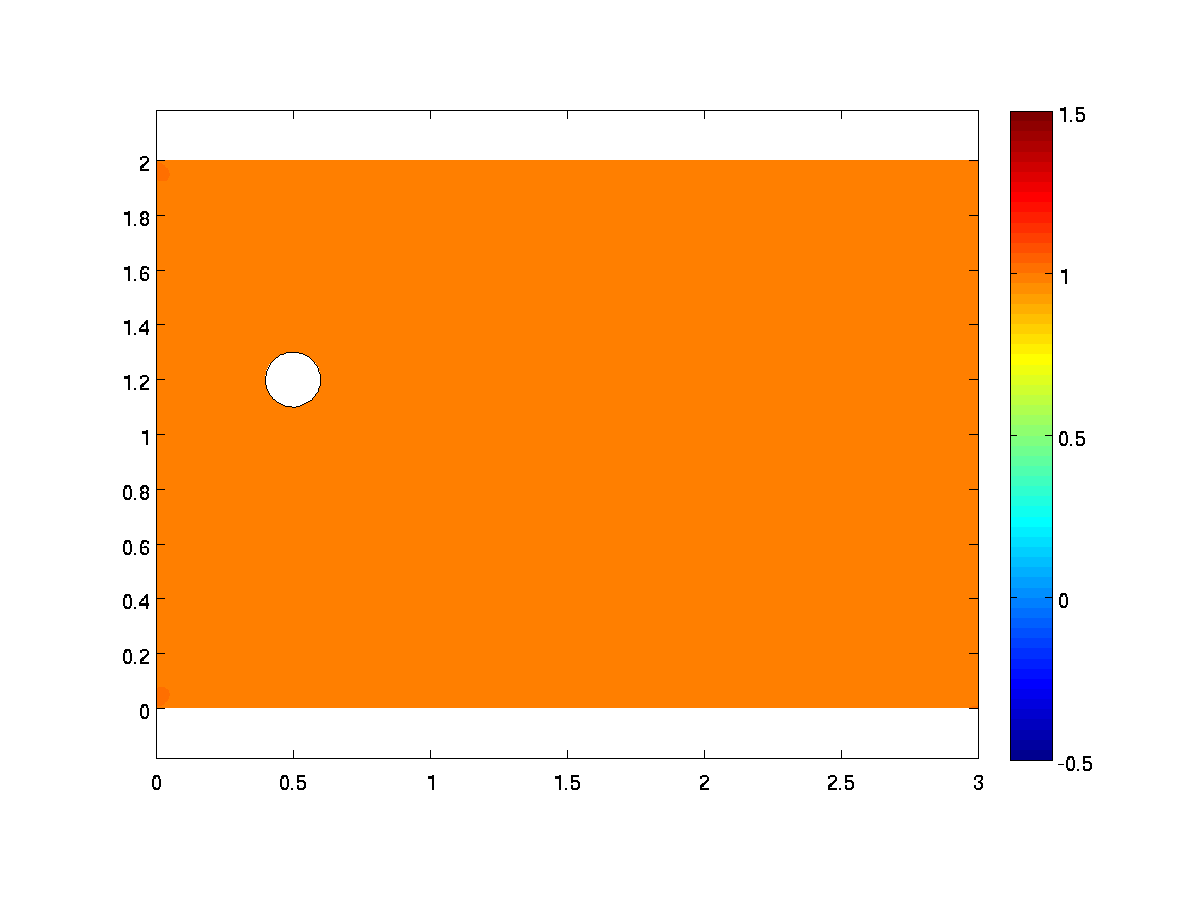
\includegraphics[width=6.0cm]{Chapter_5/figure/cylinder_analysis_Re100_t0.png}
    }
    \quad
    \subfigure[$Re = 500, t = 0 \text{ sec}$]
    {
    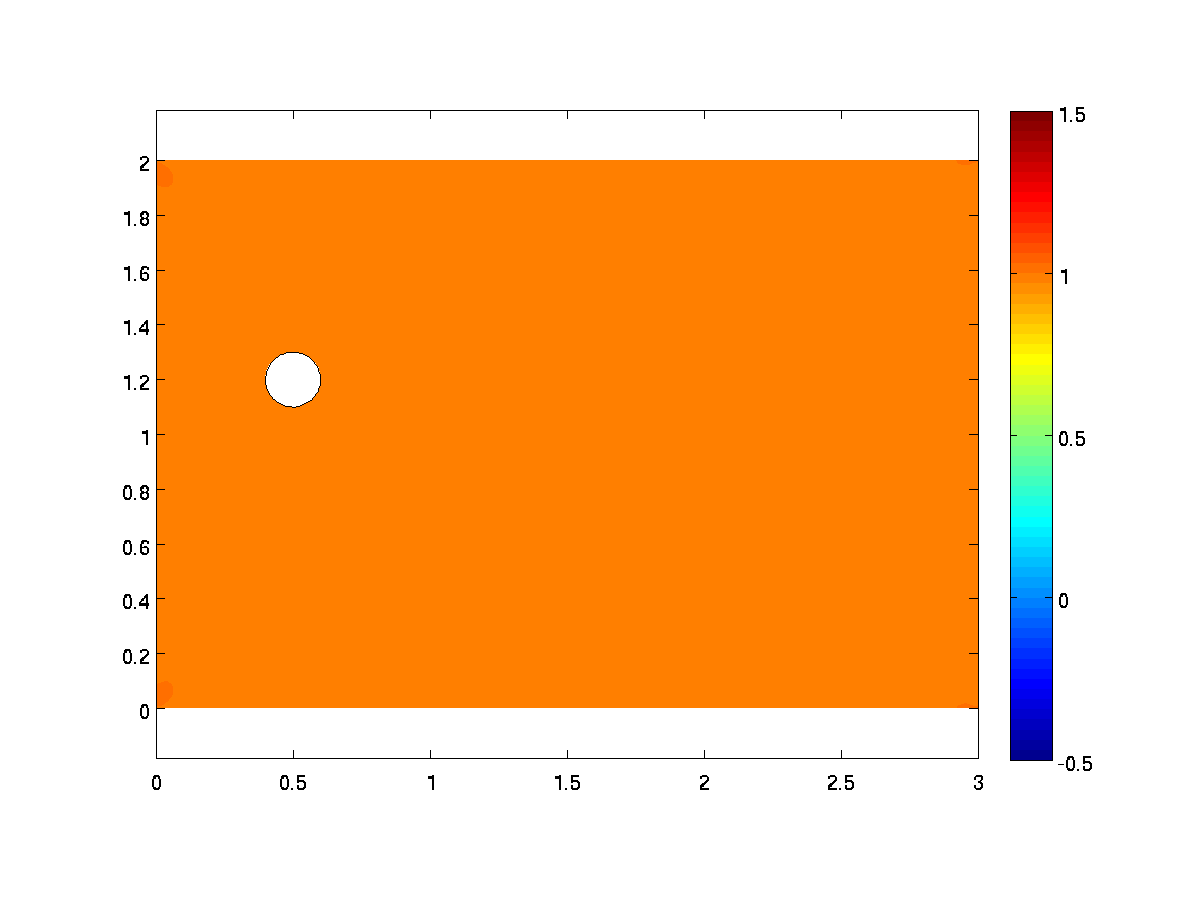
\includegraphics[width=6.0cm]{Chapter_5/figure/cylinder_analysis_Re500_t0.png}
    }
    \\
    \subfigure[$Re = 100, t = 0.5 \text{ ec}$]
    {
    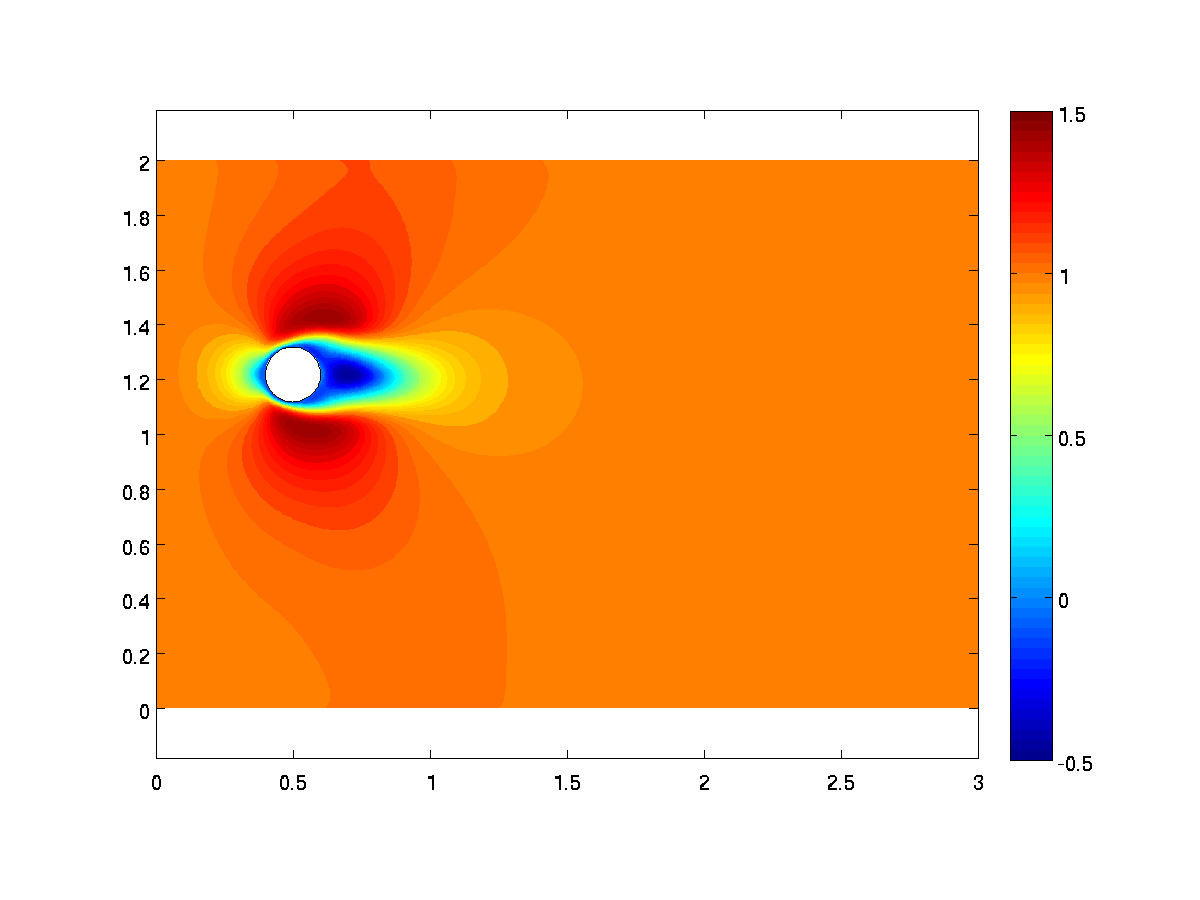
\includegraphics[width=6.0cm]{Chapter_5/figure/cylinder_analysis_Re100_t05.png}
    }
    \quad
    \subfigure[$Re = 500, t = 0.5 \text{ sec}$]
    {
    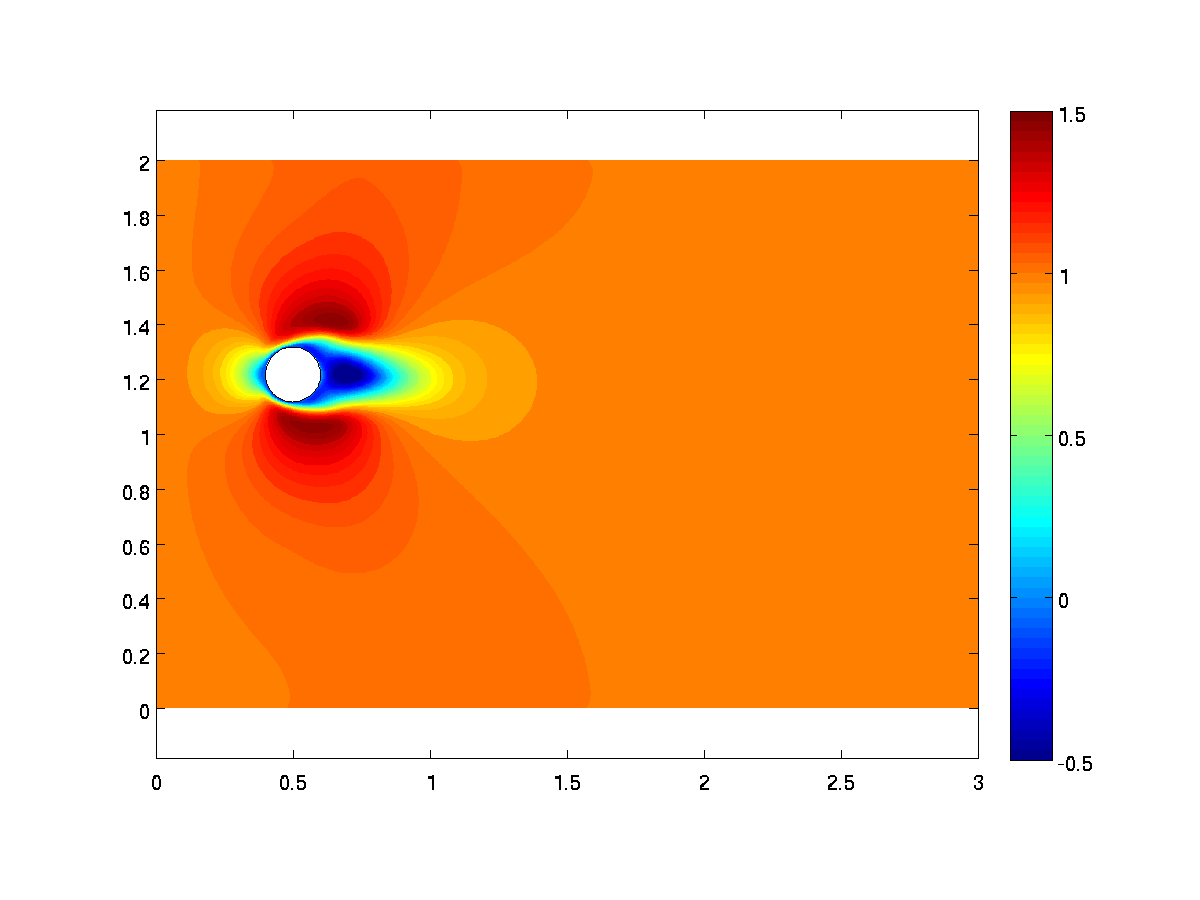
\includegraphics[width=6.0cm]{Chapter_5/figure/cylinder_analysis_Re500_t05.png}
    }
    \\
    \subfigure[$Re = 100, t = 5 \text{ sec}$]
    {
    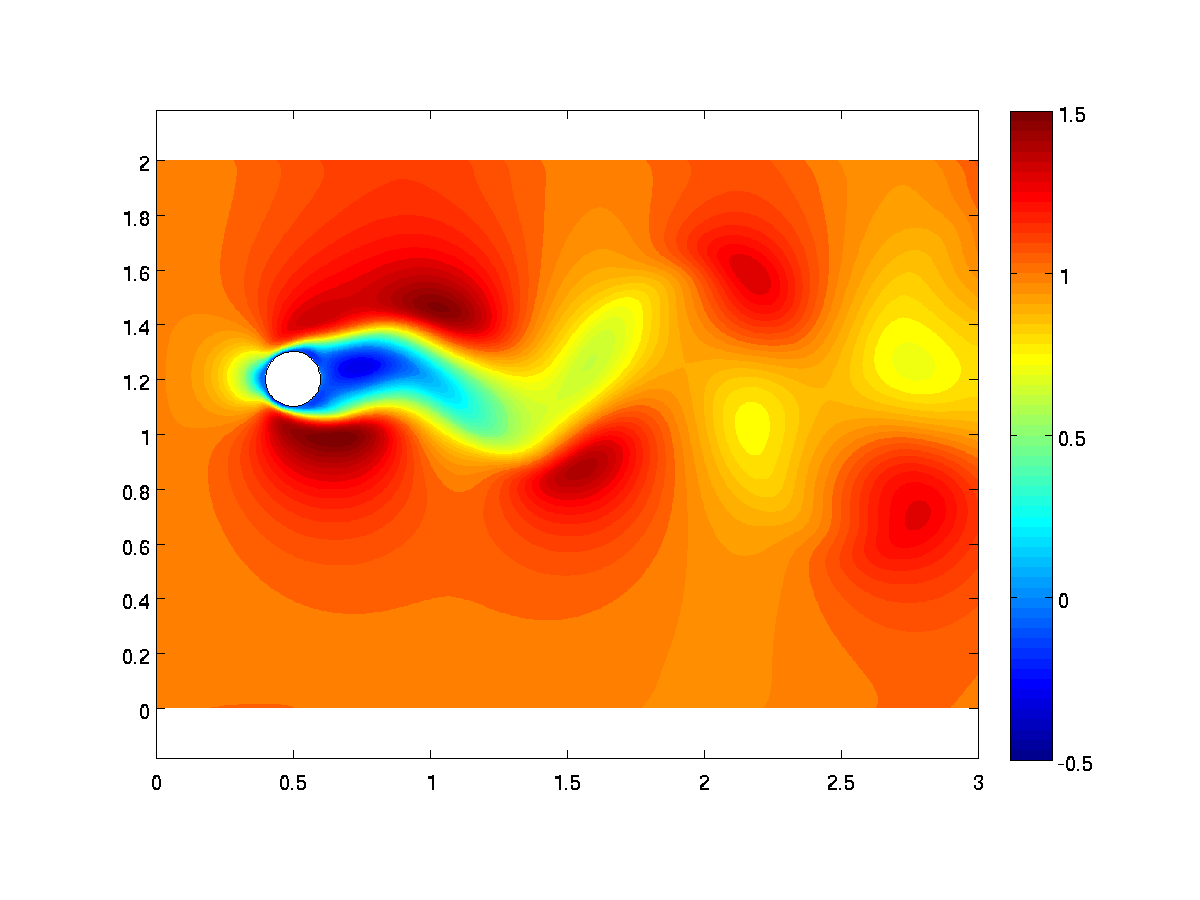
\includegraphics[width=6.0cm]{Chapter_5/figure/cylinder_analysis_Re100_t5.png}
    }
    \quad
    \subfigure[$Re = 500, t = 5 \text{ sec}$]
    {
    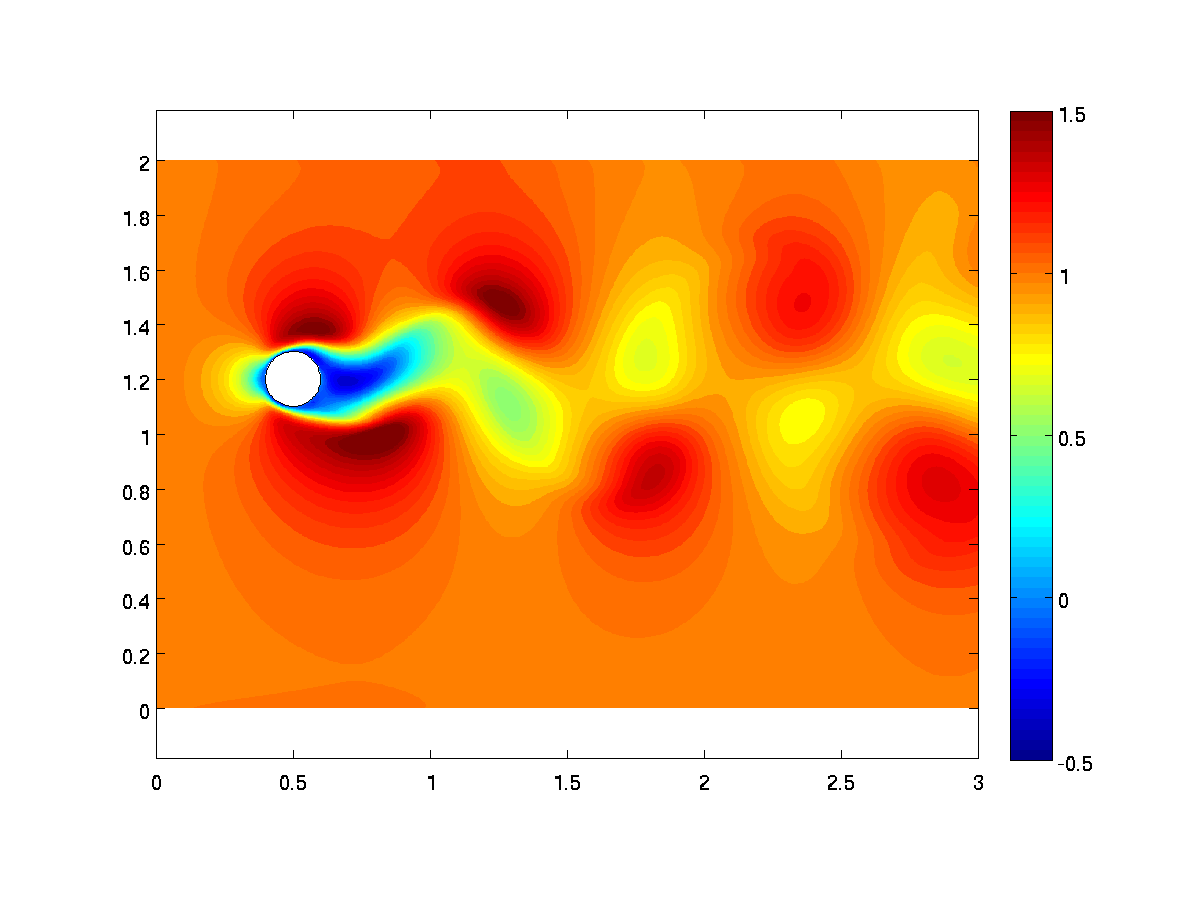
\includegraphics[width=6.0cm]{Chapter_5/figure/cylinder_analysis_Re500_t5.png}
    }
    \caption{Unsteady u-velocity contours for flow around cylinder at $Re = 100$ and $Re = 500$.}
    \label{fig:C5_cylinderFSIvelocity}
\end{figure}
%
The time history of the sensitivity results are shown and verified with the complex step solution in Figure \ref{fig:C5_cylinderDisplacementSensitivity}. As shown here, at $t=0$, the sensitivity of displacement with respect to radius is zero since the initial location of cylinder is independent of its shape. However, the value of cylinder displacement will start oscillating between positive and negative numbers as the simulation continuous. This is what we are expecting since by increasing the radius, the loads on the cylinder will increase. This will result in an increase in the amplitude in both ends of the oscillation period.
%
\begin{figure}[H]
    \centering
    \subfigure[$Re = 100$]
    {
    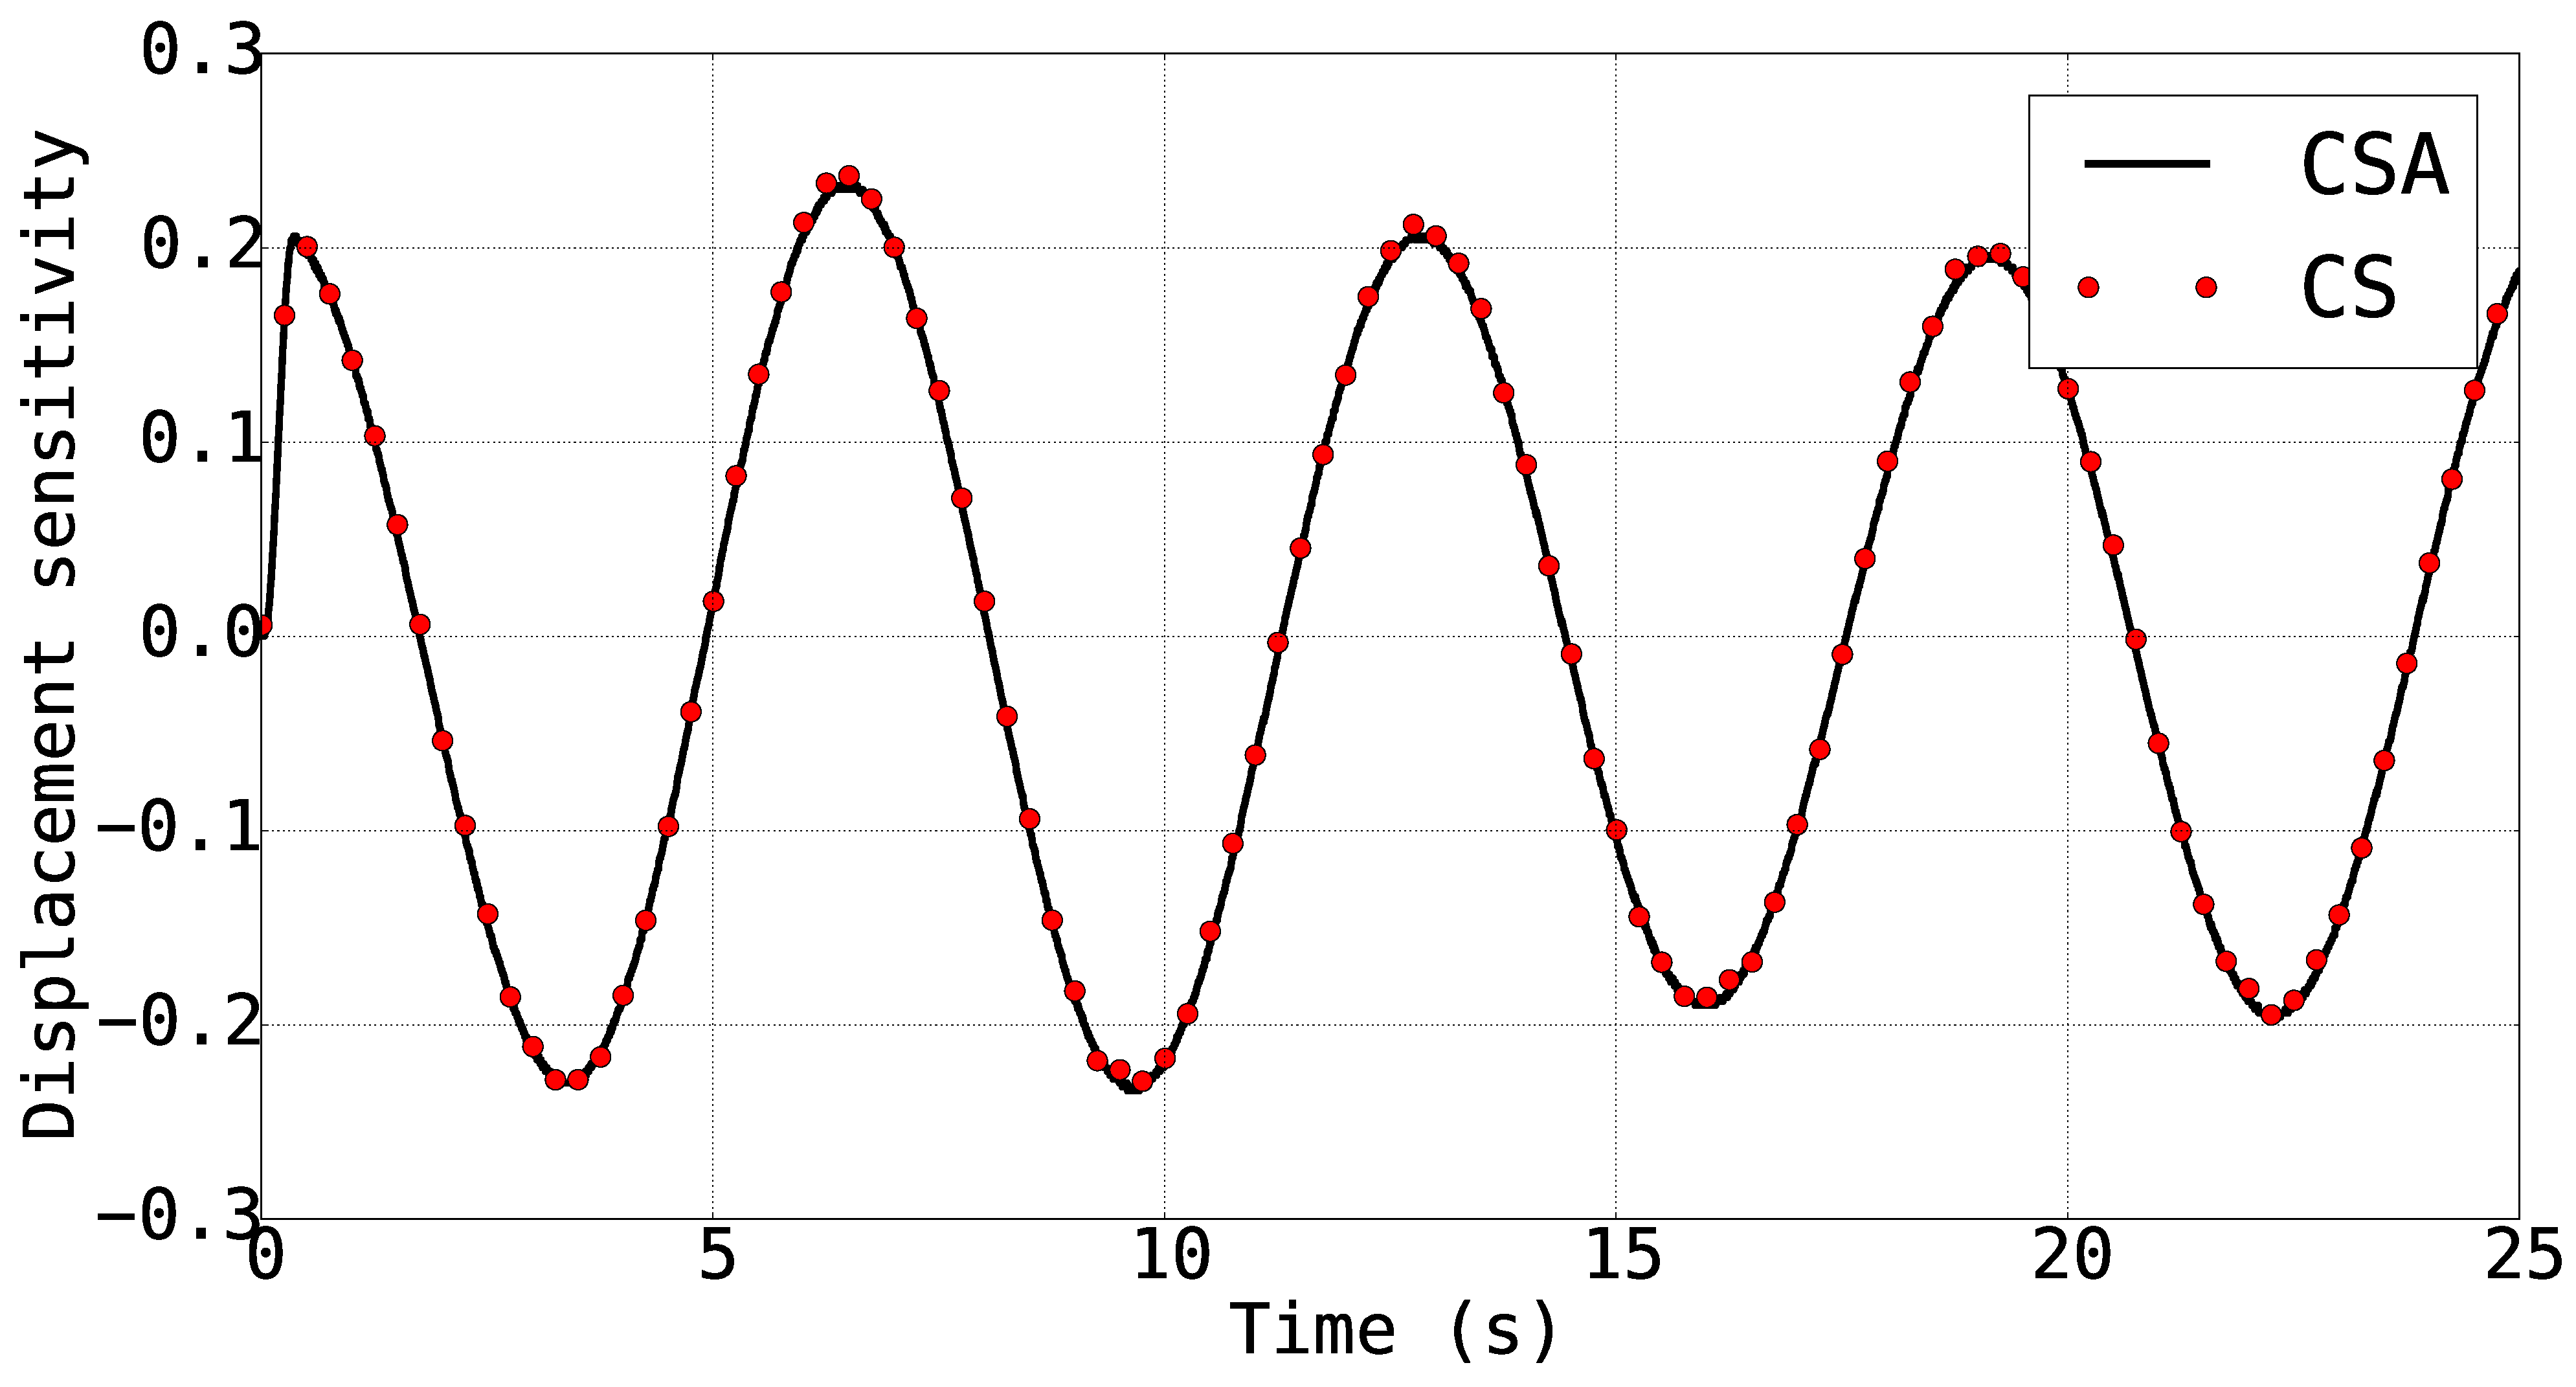
\includegraphics[width=9.0cm]{Chapter_5/figure/cylinder_Re100_DisplacementSensitivity.eps}
    }
    \quad
    \subfigure[$Re = 500$]
    {
    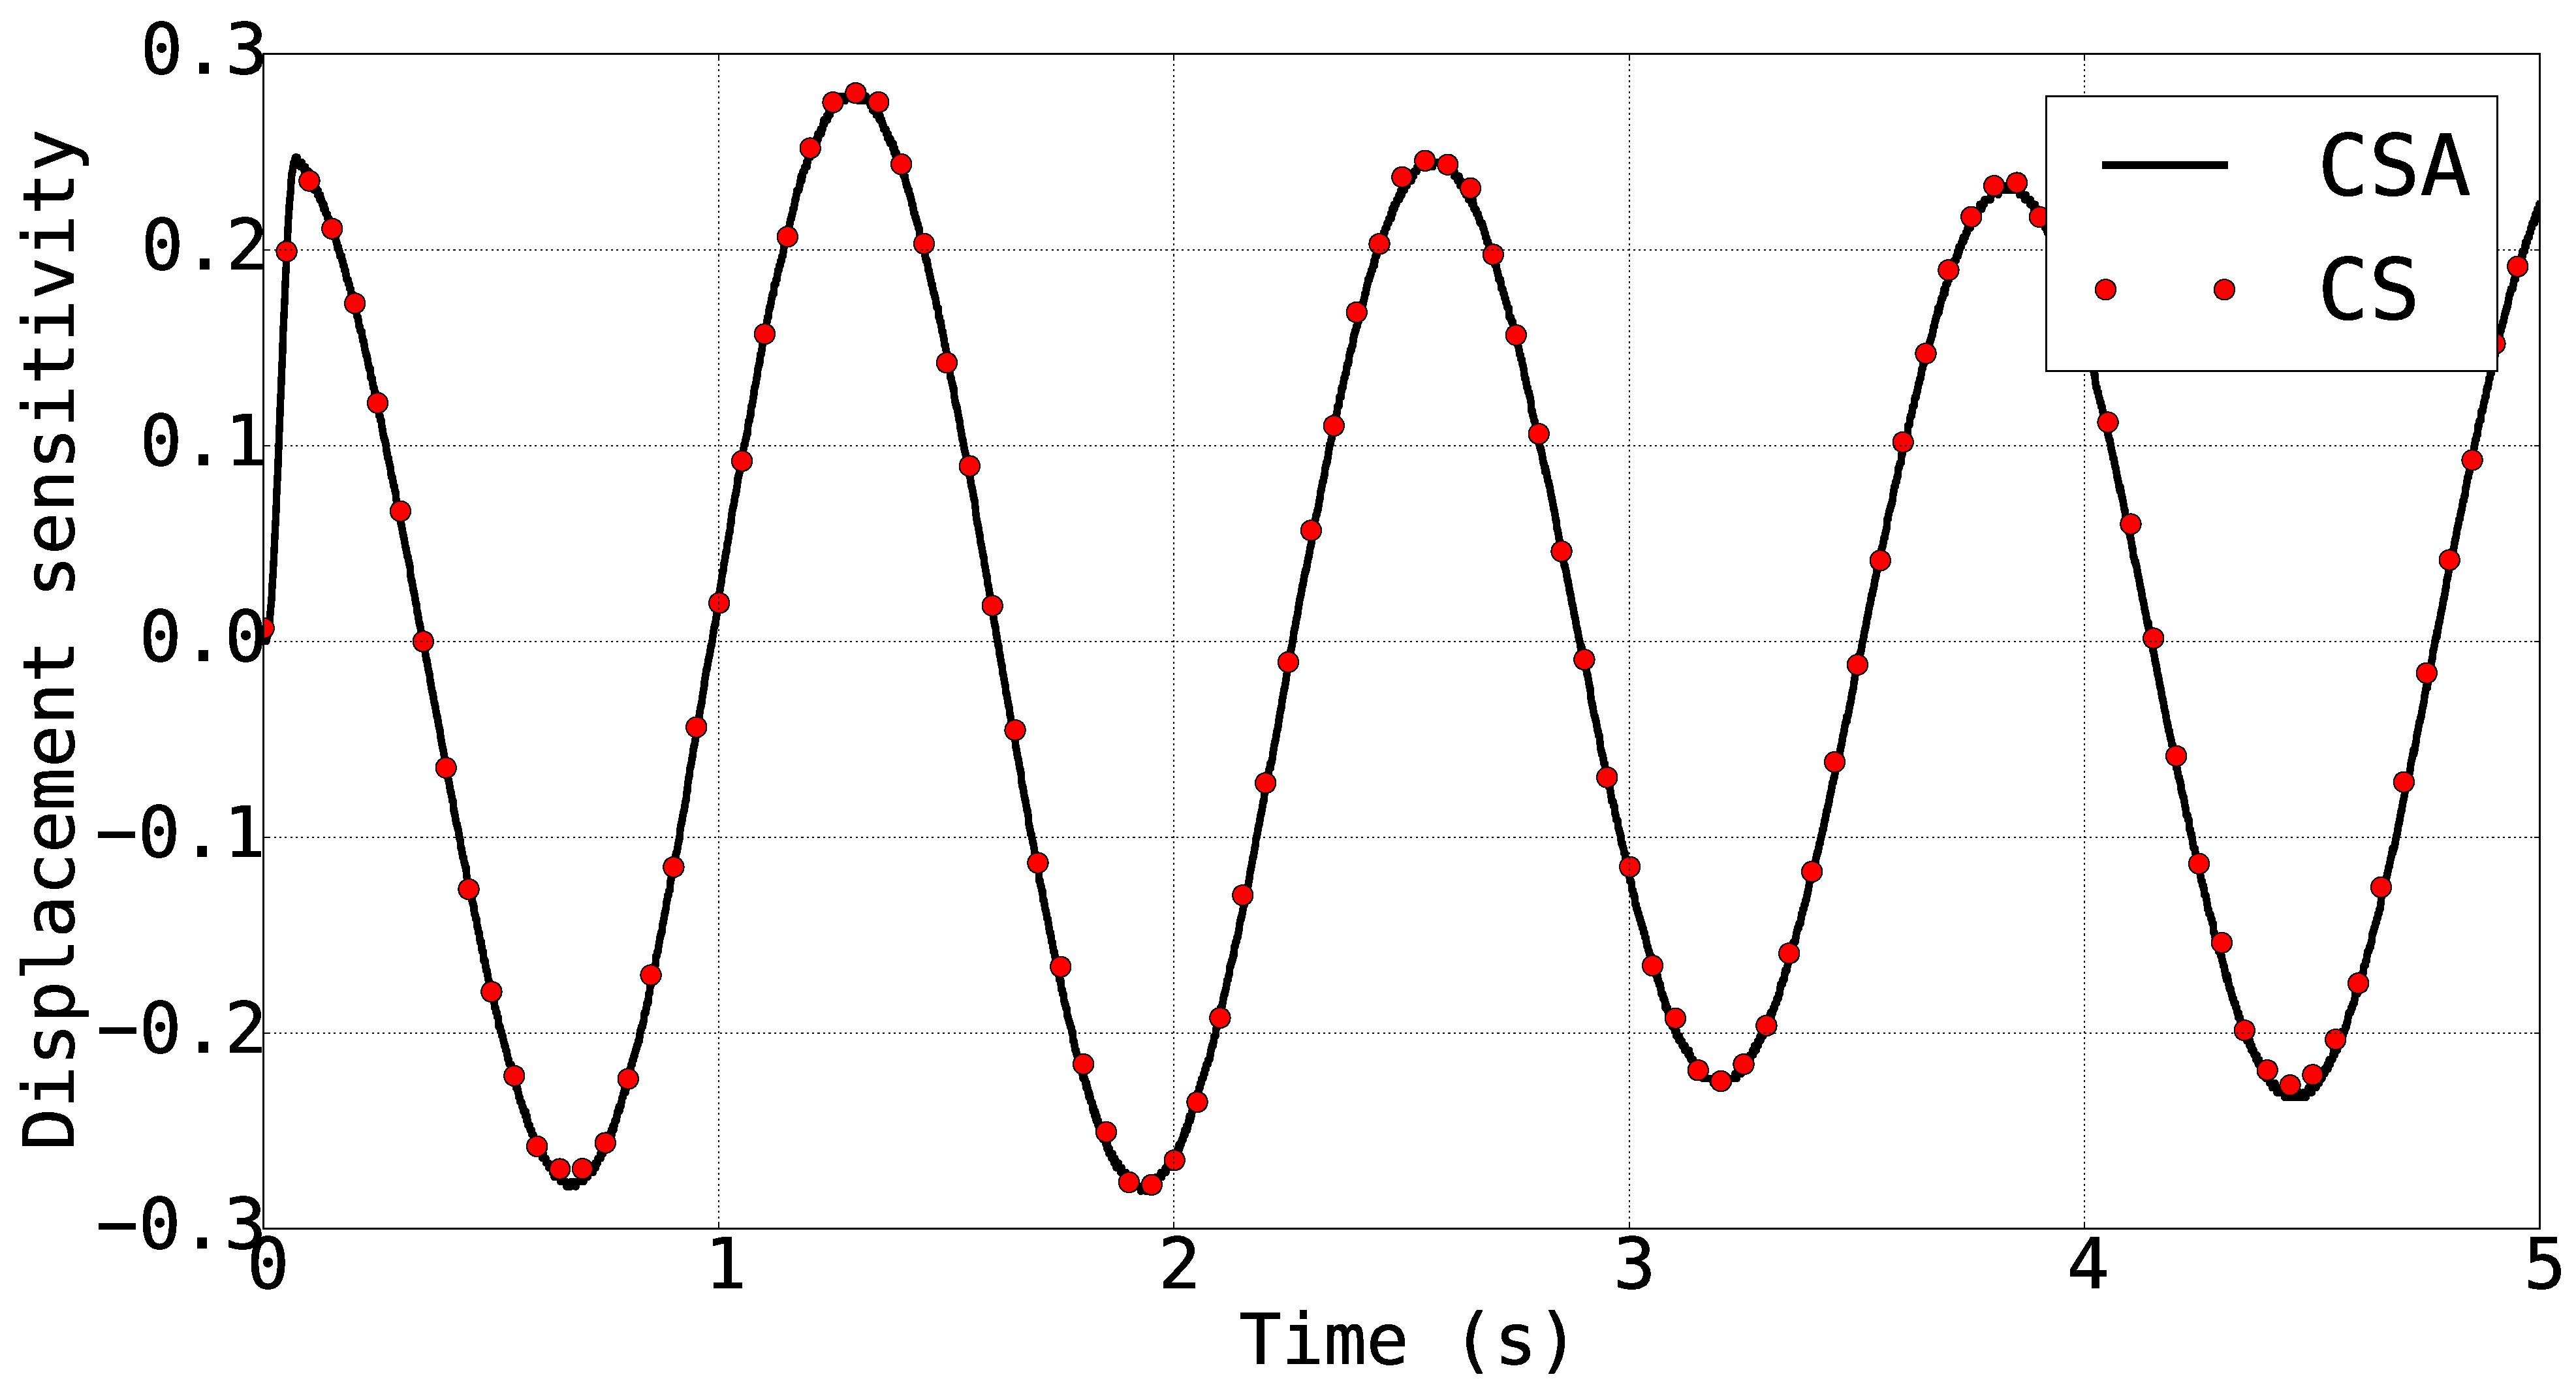
\includegraphics[width=9.0cm]{Chapter_5/figure/cylinder_Re500_DisplacementSensitivity.eps}
    }
    \caption{Time history of cylinder center displacement sensitivity.}
    \label{fig:C5_cylinderDisplacementSensitivity}
\end{figure}
%
Figure \ref{fig:C5_cylinderFSIvelocitySensitivity} shows the u-velocity sensitivity contour around the elastically mounted cylinder at different times. As shown in the sensitivity contours, the change in the cylinder radius mainly affects the downstream flow. This is expected for a convective flow where information from the cylinder cannot move upstream. The small region with negative sensitivity near the surface is due to the reduction of velocity due to boundary layer expansion as the radius increases and has physical meaning.
%
\begin{figure}[H]
    \centering
    \subfigure[$Re = 100, t = 0 \text{ sec}$]
    {
    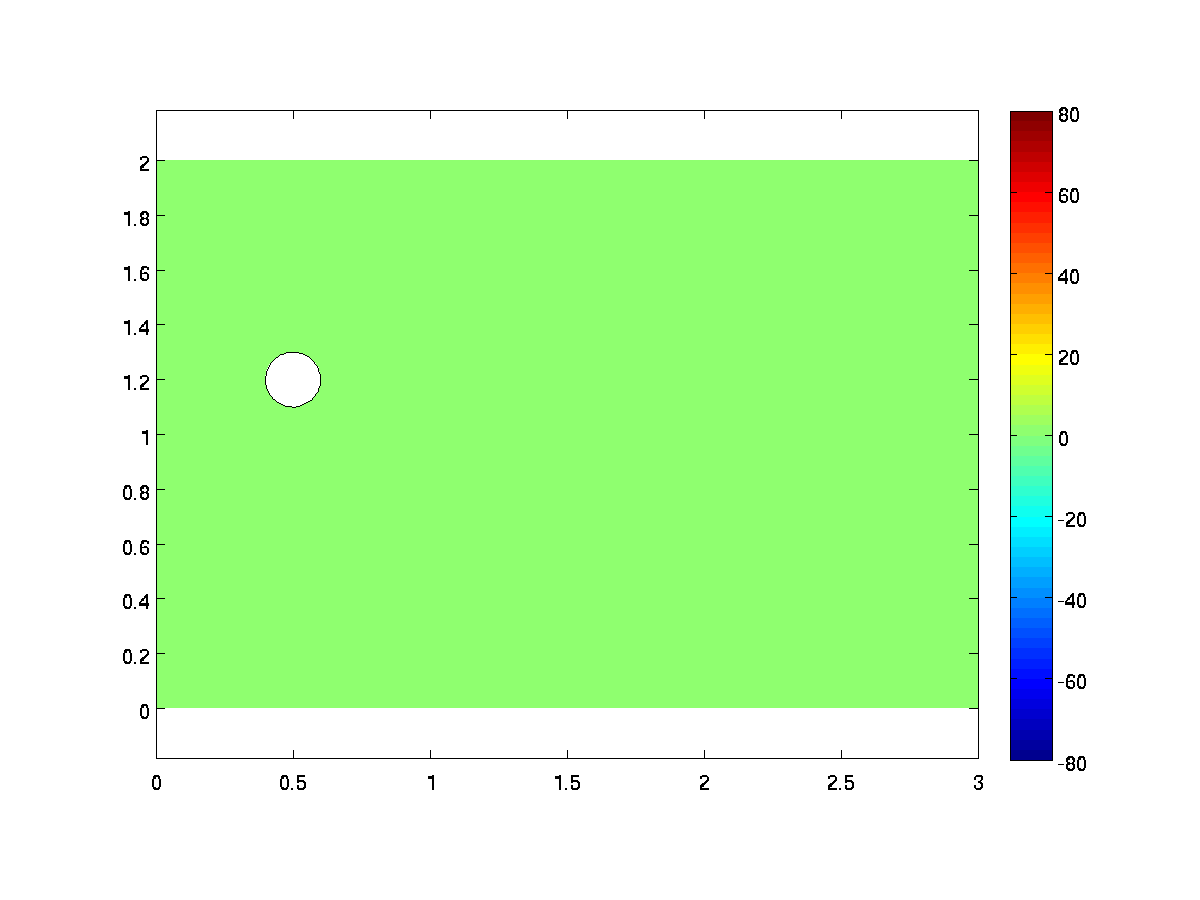
\includegraphics[width=6.0cm]{Chapter_5/figure/cylinder_sensitivity_Re100_t0.png}
    }
    \quad
    \subfigure[$Re = 500, t = 0 \text{ sec}$]
    {
    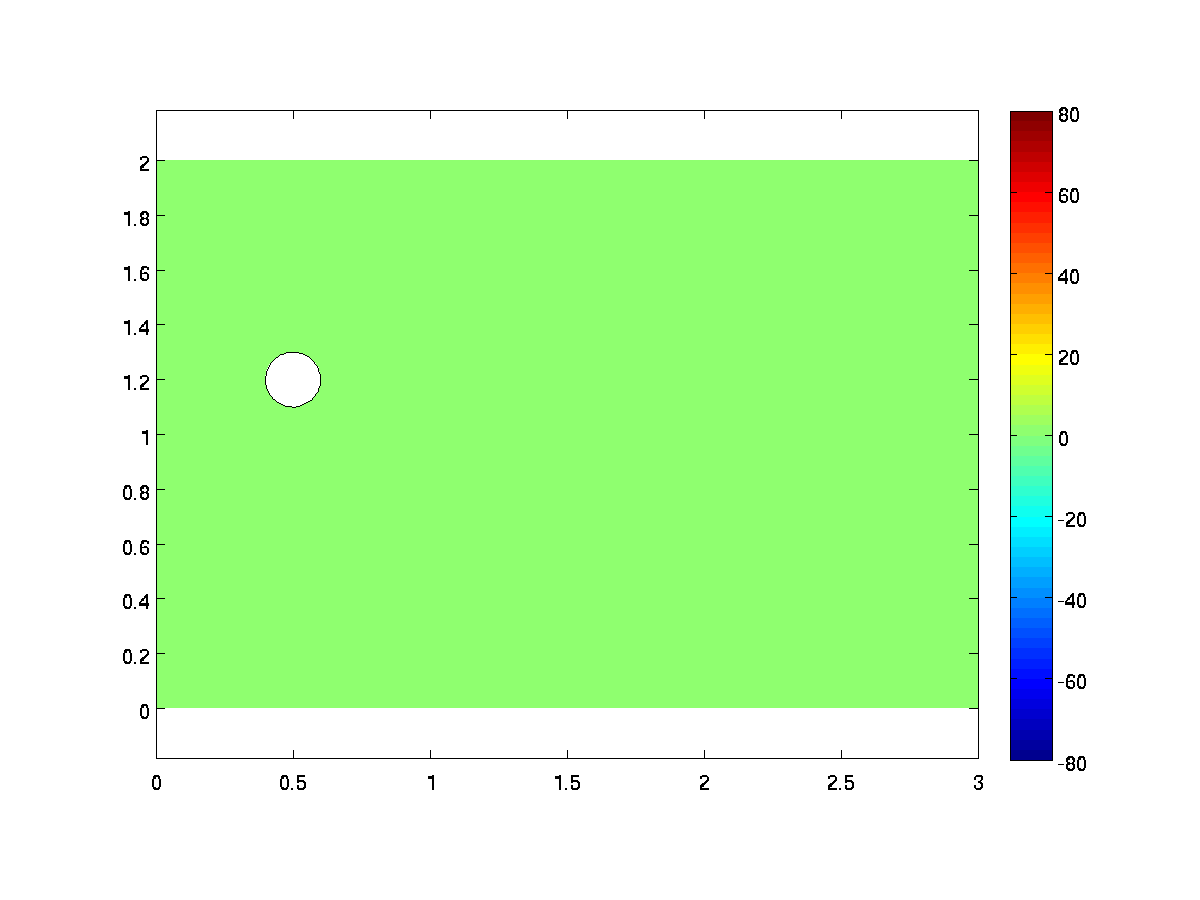
\includegraphics[width=6.0cm]{Chapter_5/figure/cylinder_sensitivity_Re500_t0.png}
    }
    \\
    \subfigure[$Re = 100, t = 0.5 \text{ ec}$]
    {
    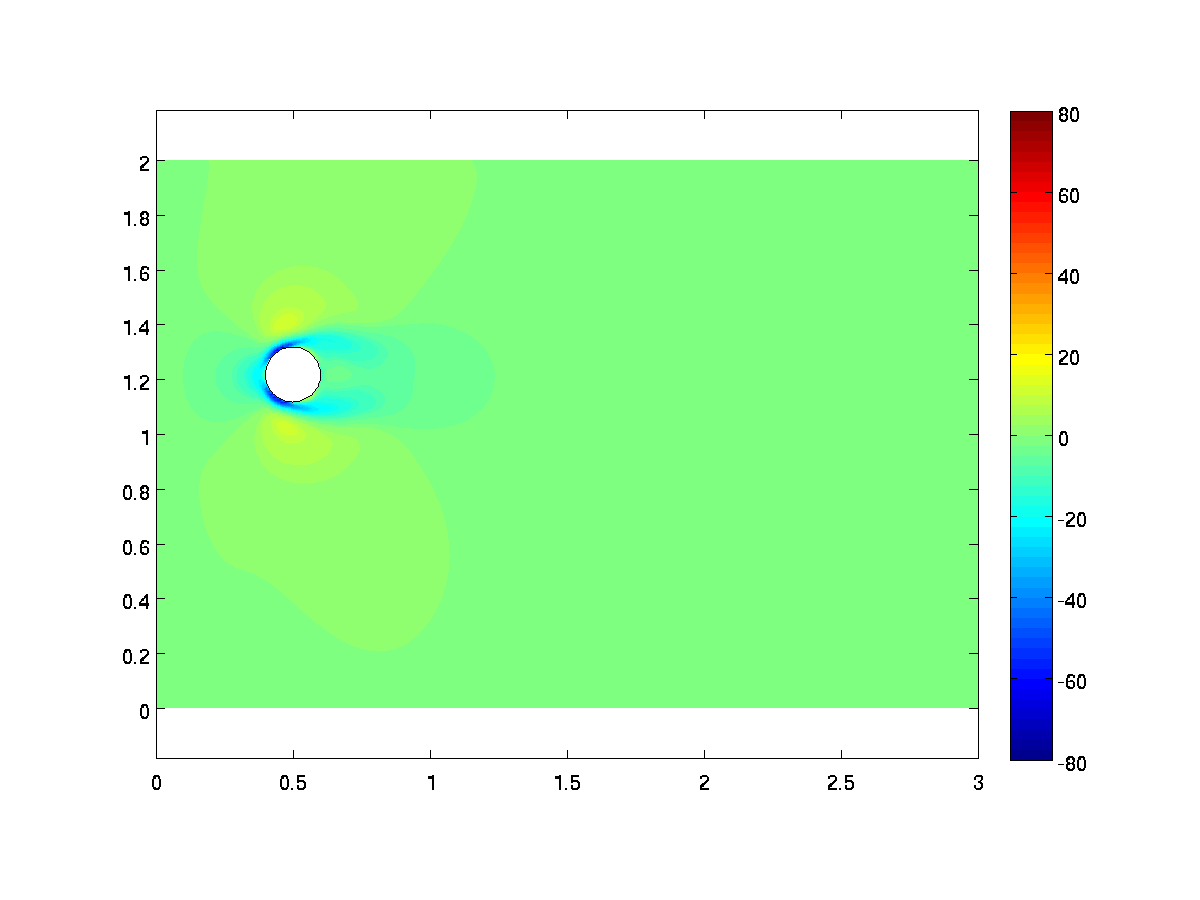
\includegraphics[width=6.0cm]{Chapter_5/figure/cylinder_sensitivity_Re100_t05.png}
    }
    \quad
    \subfigure[$Re = 500, t = 0.5 \text{ sec}$]
    {
    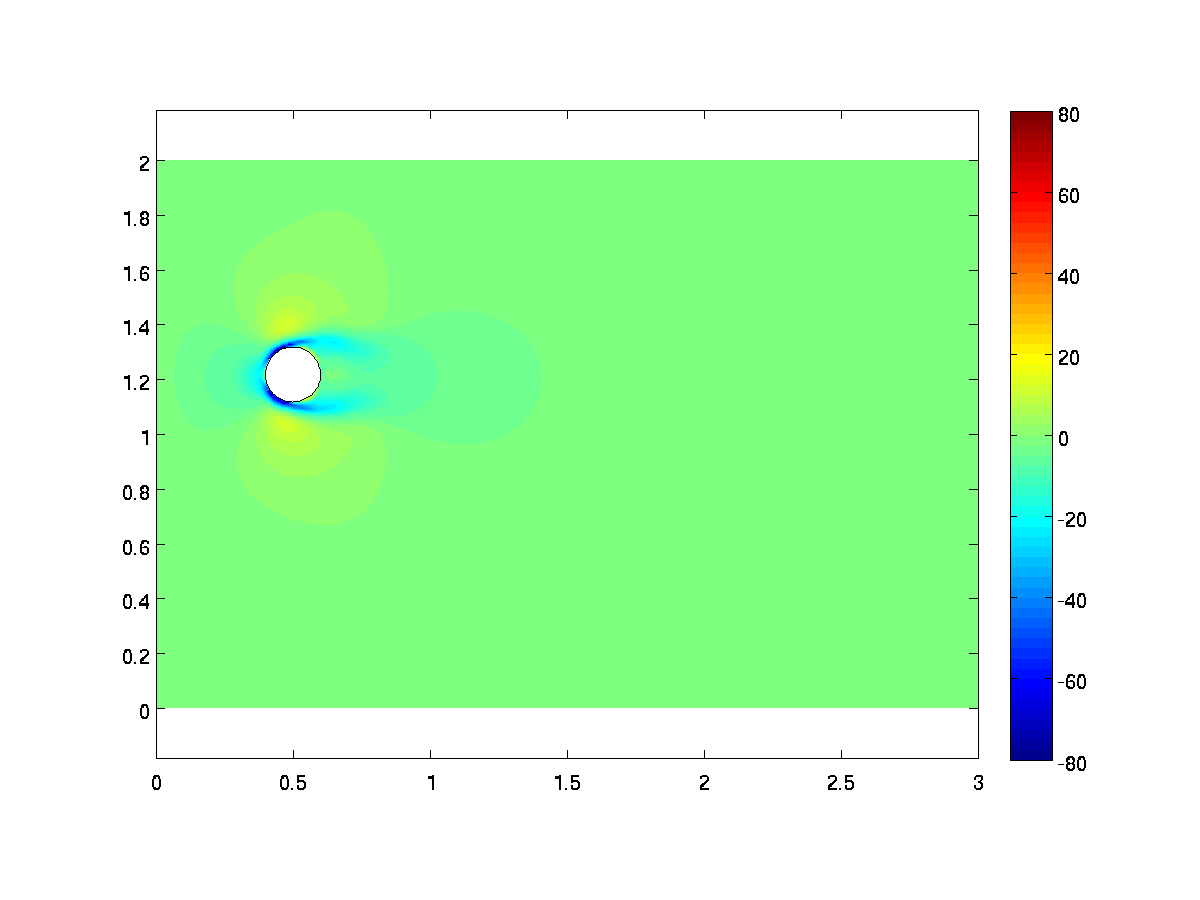
\includegraphics[width=6.0cm]{Chapter_5/figure/cylinder_sensitivity_Re500_t05.png}
    }
    \\
    \subfigure[$Re = 100, t = 5 \text{ sec}$]
    {
    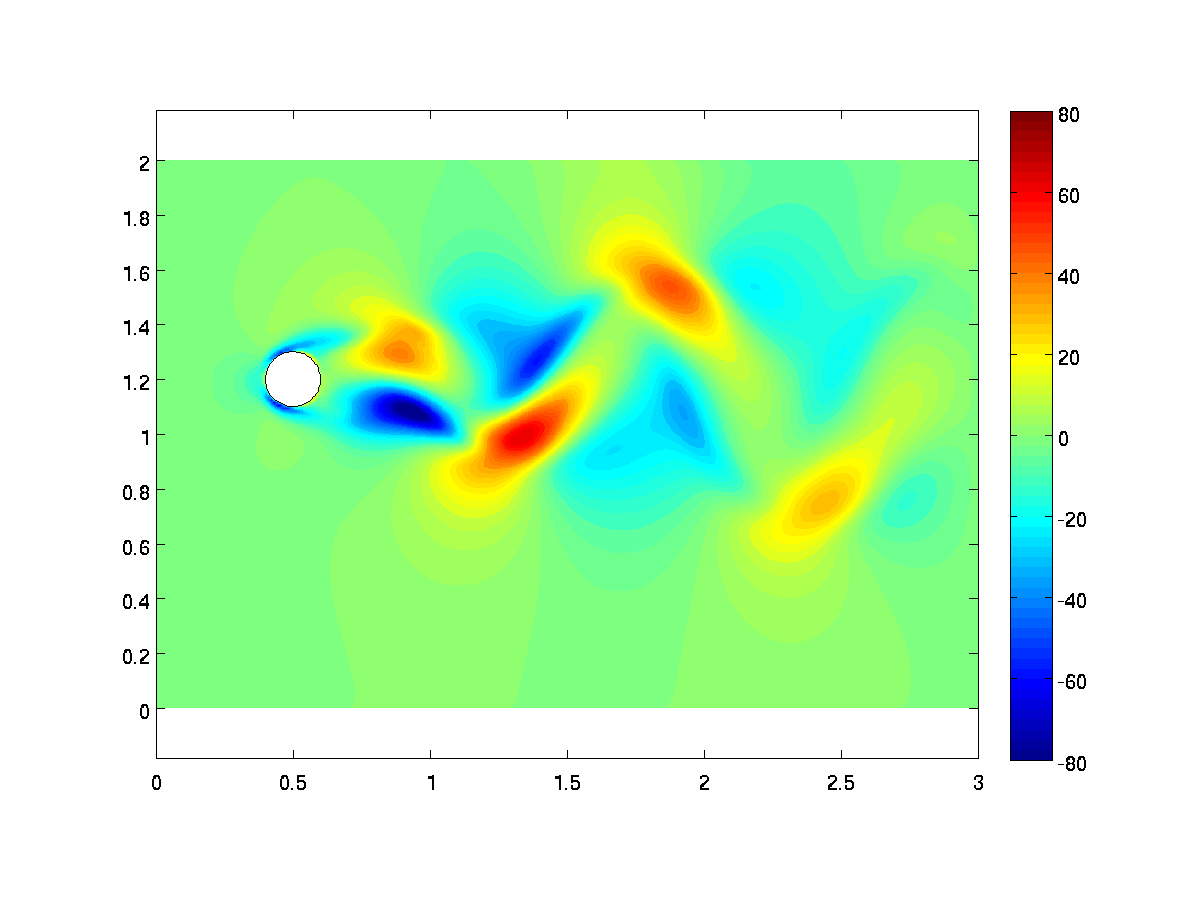
\includegraphics[width=6.0cm]{Chapter_5/figure/cylinder_sensitivity_Re100_t5.png}
    }
    \quad
    \subfigure[$Re = 500, t = 5 \text{ sec}$]
    {
    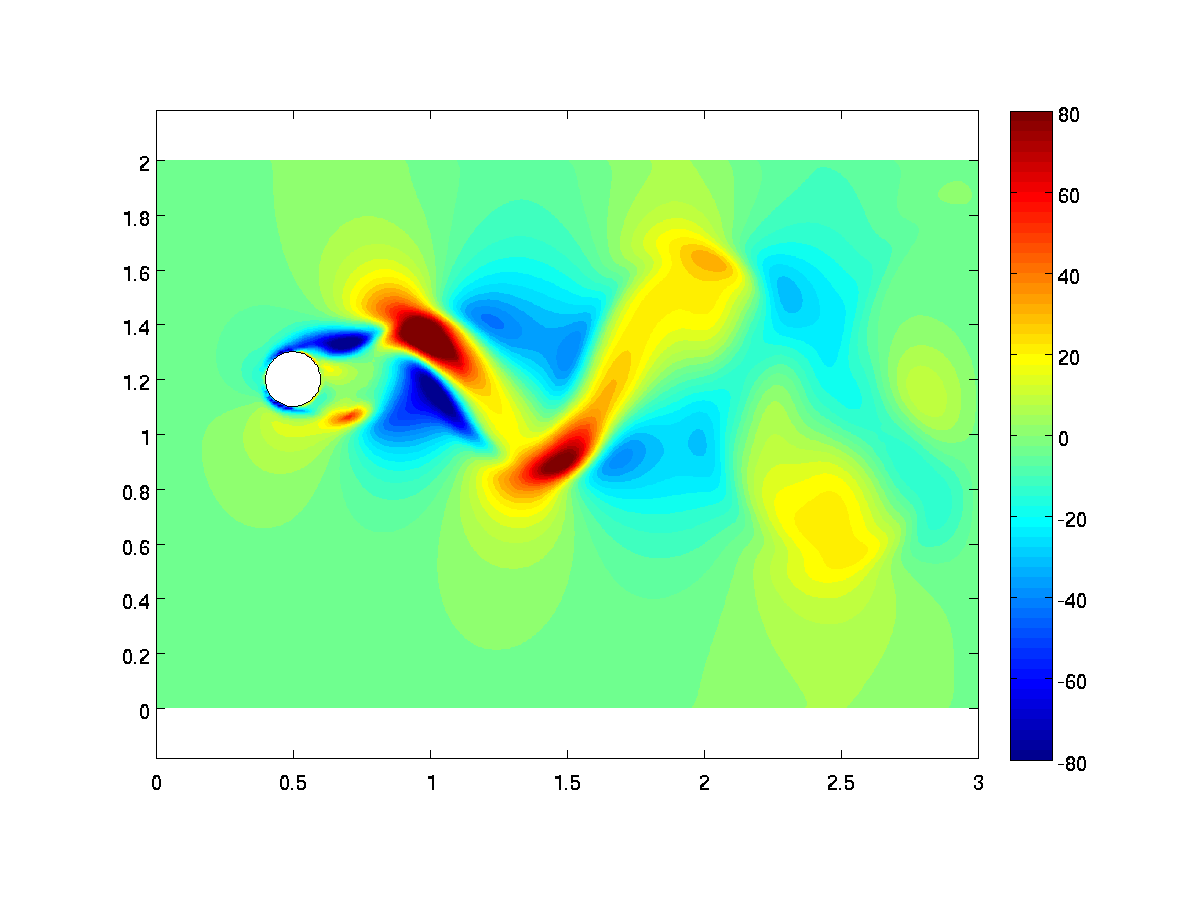
\includegraphics[width=6.0cm]{Chapter_5/figure/cylinder_sensitivity_Re500_t5.png}
    }
    \caption{Unsteady u-velocity contours for flow around cylinder at $Re = 100$ and $Re = 500$.}
    \label{fig:C5_cylinderFSIvelocitySensitivity}
\end{figure}
%
\subsection{Pitch and Plunge Airfoil Motion}
Understanding the unsteady aerodynamic characteristics of a pitching and plunging airfoil has two major engineering applications. First, it can be used to predict the dynamic stall of aerodynamic bodies such as aircraft in a demanding maneuver \cite{tuncer1998computational}. Dynamic stall is often seen in aerodynamic surfaces going through a pitching moment or oscillatory behavior. This phenomenon is caused due to instability and separation of the leading-edge vortex which results in a dramatic decrease in lift and sudden increase in pitching moment. Dynamic stall can lead to high amplitude vibrations and high loads that can cause fatigue and structural failure of the aerodynamic surfaces. The second motivation of investigating this unsteady aerodynamic behavior is the application of flapping wings for swimming and flying animals \cite{shyy2008computational}. The vast majority of research on the pitching and plunging airfoil is done by forcing the motion on the airfoil and looking at the aerodynamic response. This is mainly done for investigating the thrust and the parameters that control it \cite{tuncer2000computational, lian2008comparative}. Webb, et al. investigated the use of IB method for the forced pitching and plunging movement of the SD7003 airfoil and verified their solution with experimental results \cite{webb2008effects}. In this work, we are interested in the free oscillations of the airfoil due to aerodynamic loads. Moreover, we will investigate sensitivity of the airfoil displacement to its shape.

To have an analytical representation of the airfoil shape, we used the Joukowsky transform to define the geometry. Joukowsky transform is a conformal mapping that maps a circle in the complex plane to a shape that represents a typical airfoil shape. The Joukowsky transform is shown in Equation \eqref{eq:C5_joukowskyTransform}.
%
\begin{equation}\label{eq:C5_joukowskyTransform}
	z = \zeta + \frac{1}{\zeta} \quad , \quad \zeta = x + iy
\end{equation}
%
As shown in Figure \ref{fig:C5_joukowskyAirfoil}, the center location of the original circle defines the thickness and camber of the airfoil. For the sensitivity analysis, we are interested in the sensitivity of flow to the chamber; therefore, it is required to differentiate with the $y$ coordinate of circle center. This is calculated analytically.
%
\begin{figure}[H]
    \centering
    \subfigure[$x_c = 0.05, y_c = 0.0$]
    {
    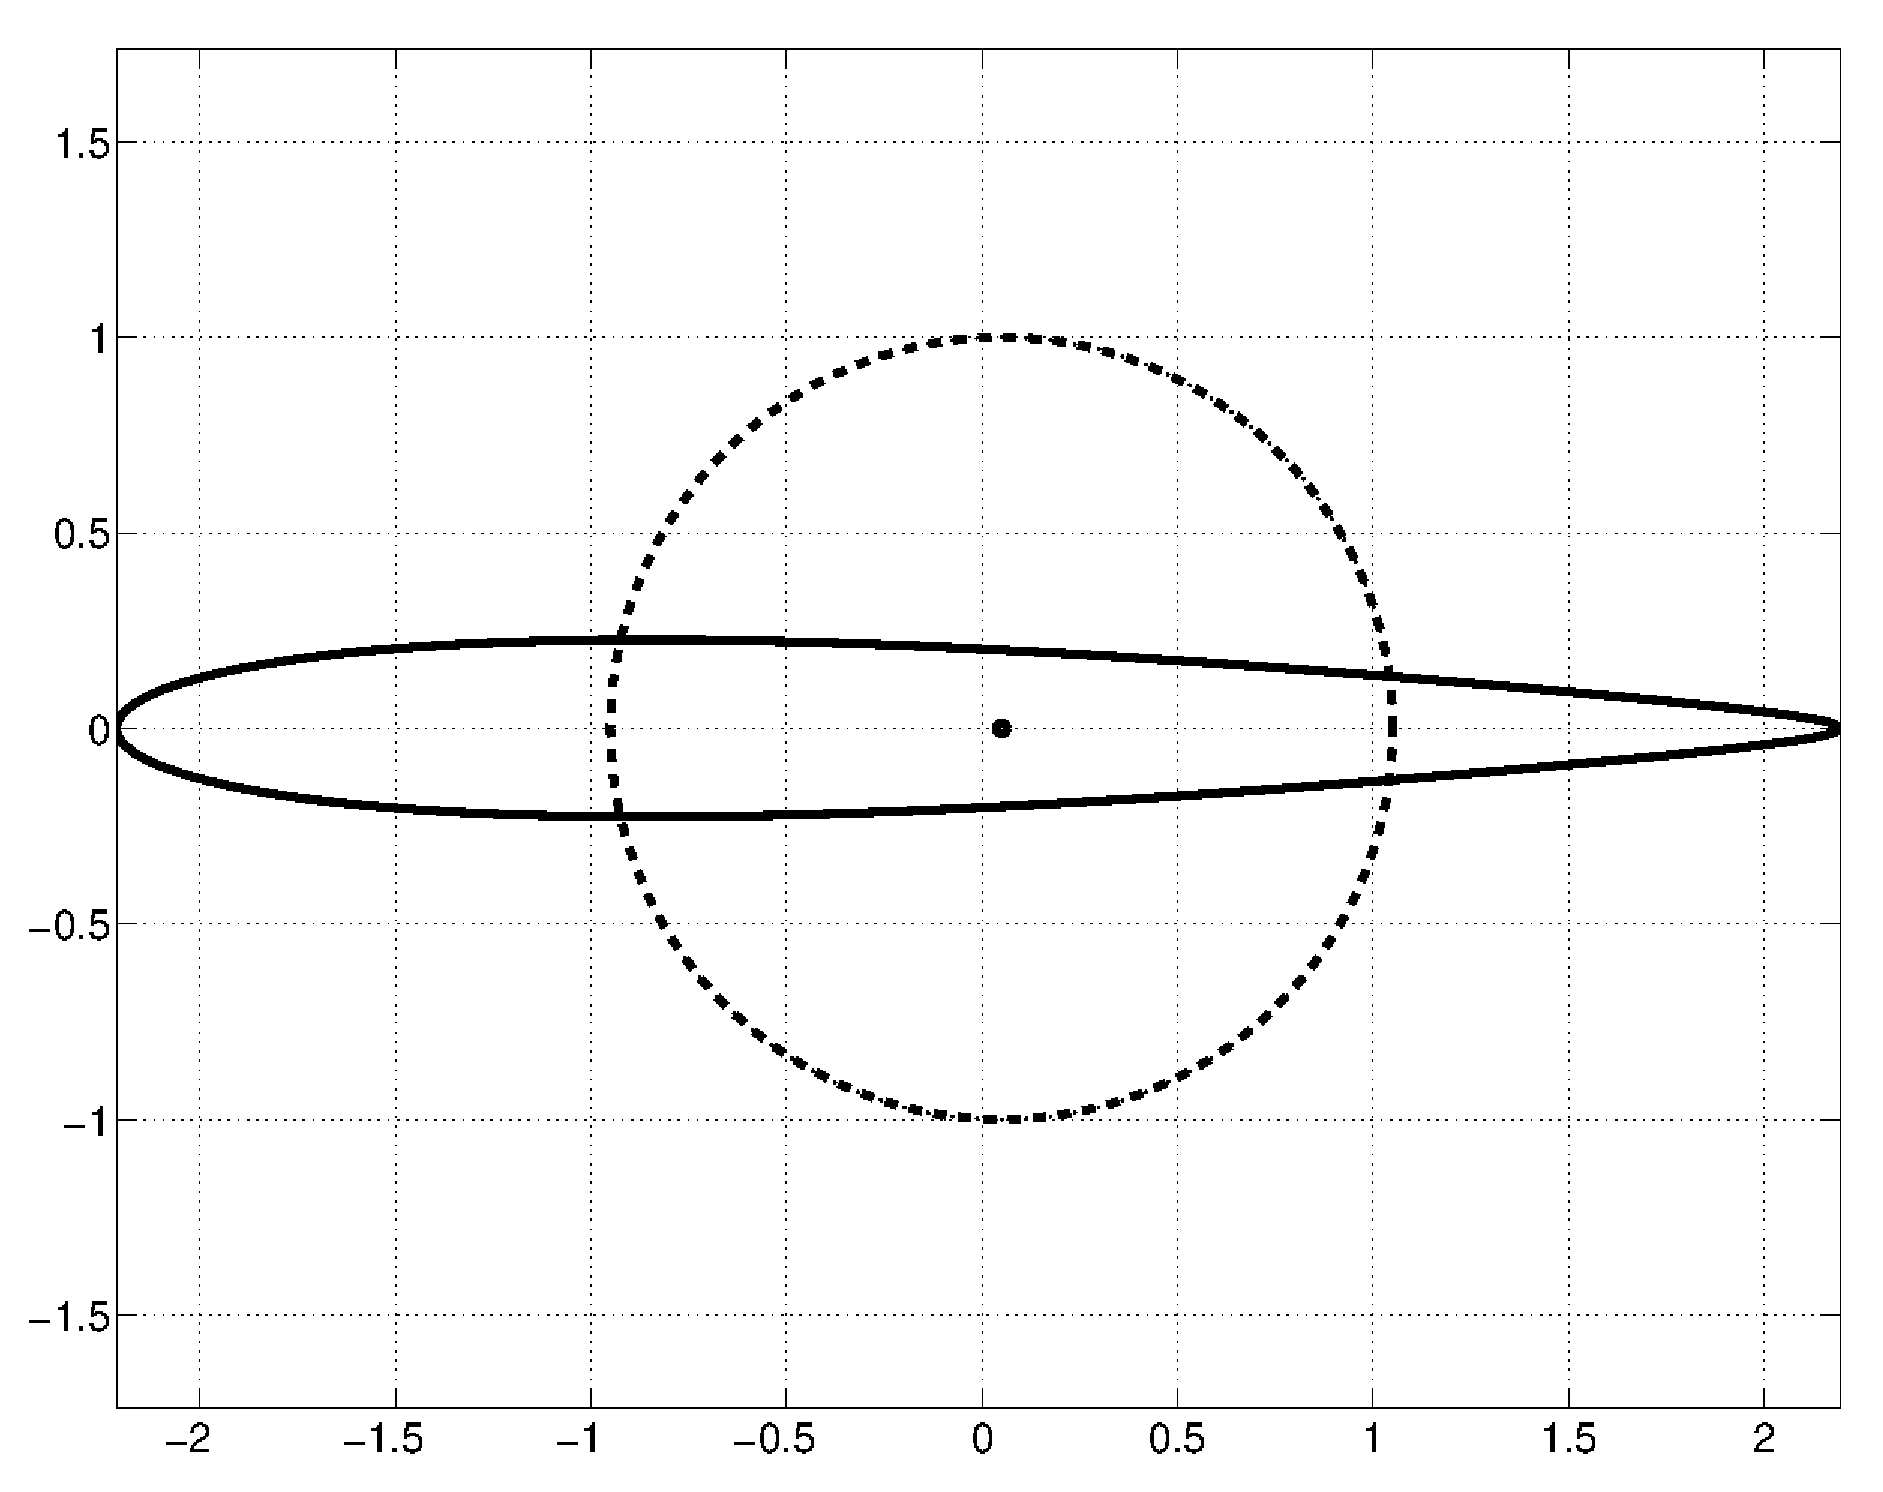
\includegraphics[width=4.25cm]{Chapter_5/figure/airfoil_base.eps}
    }
    \quad
    \subfigure[$x_c = 0.05, y_c = 0.1$]
    {
    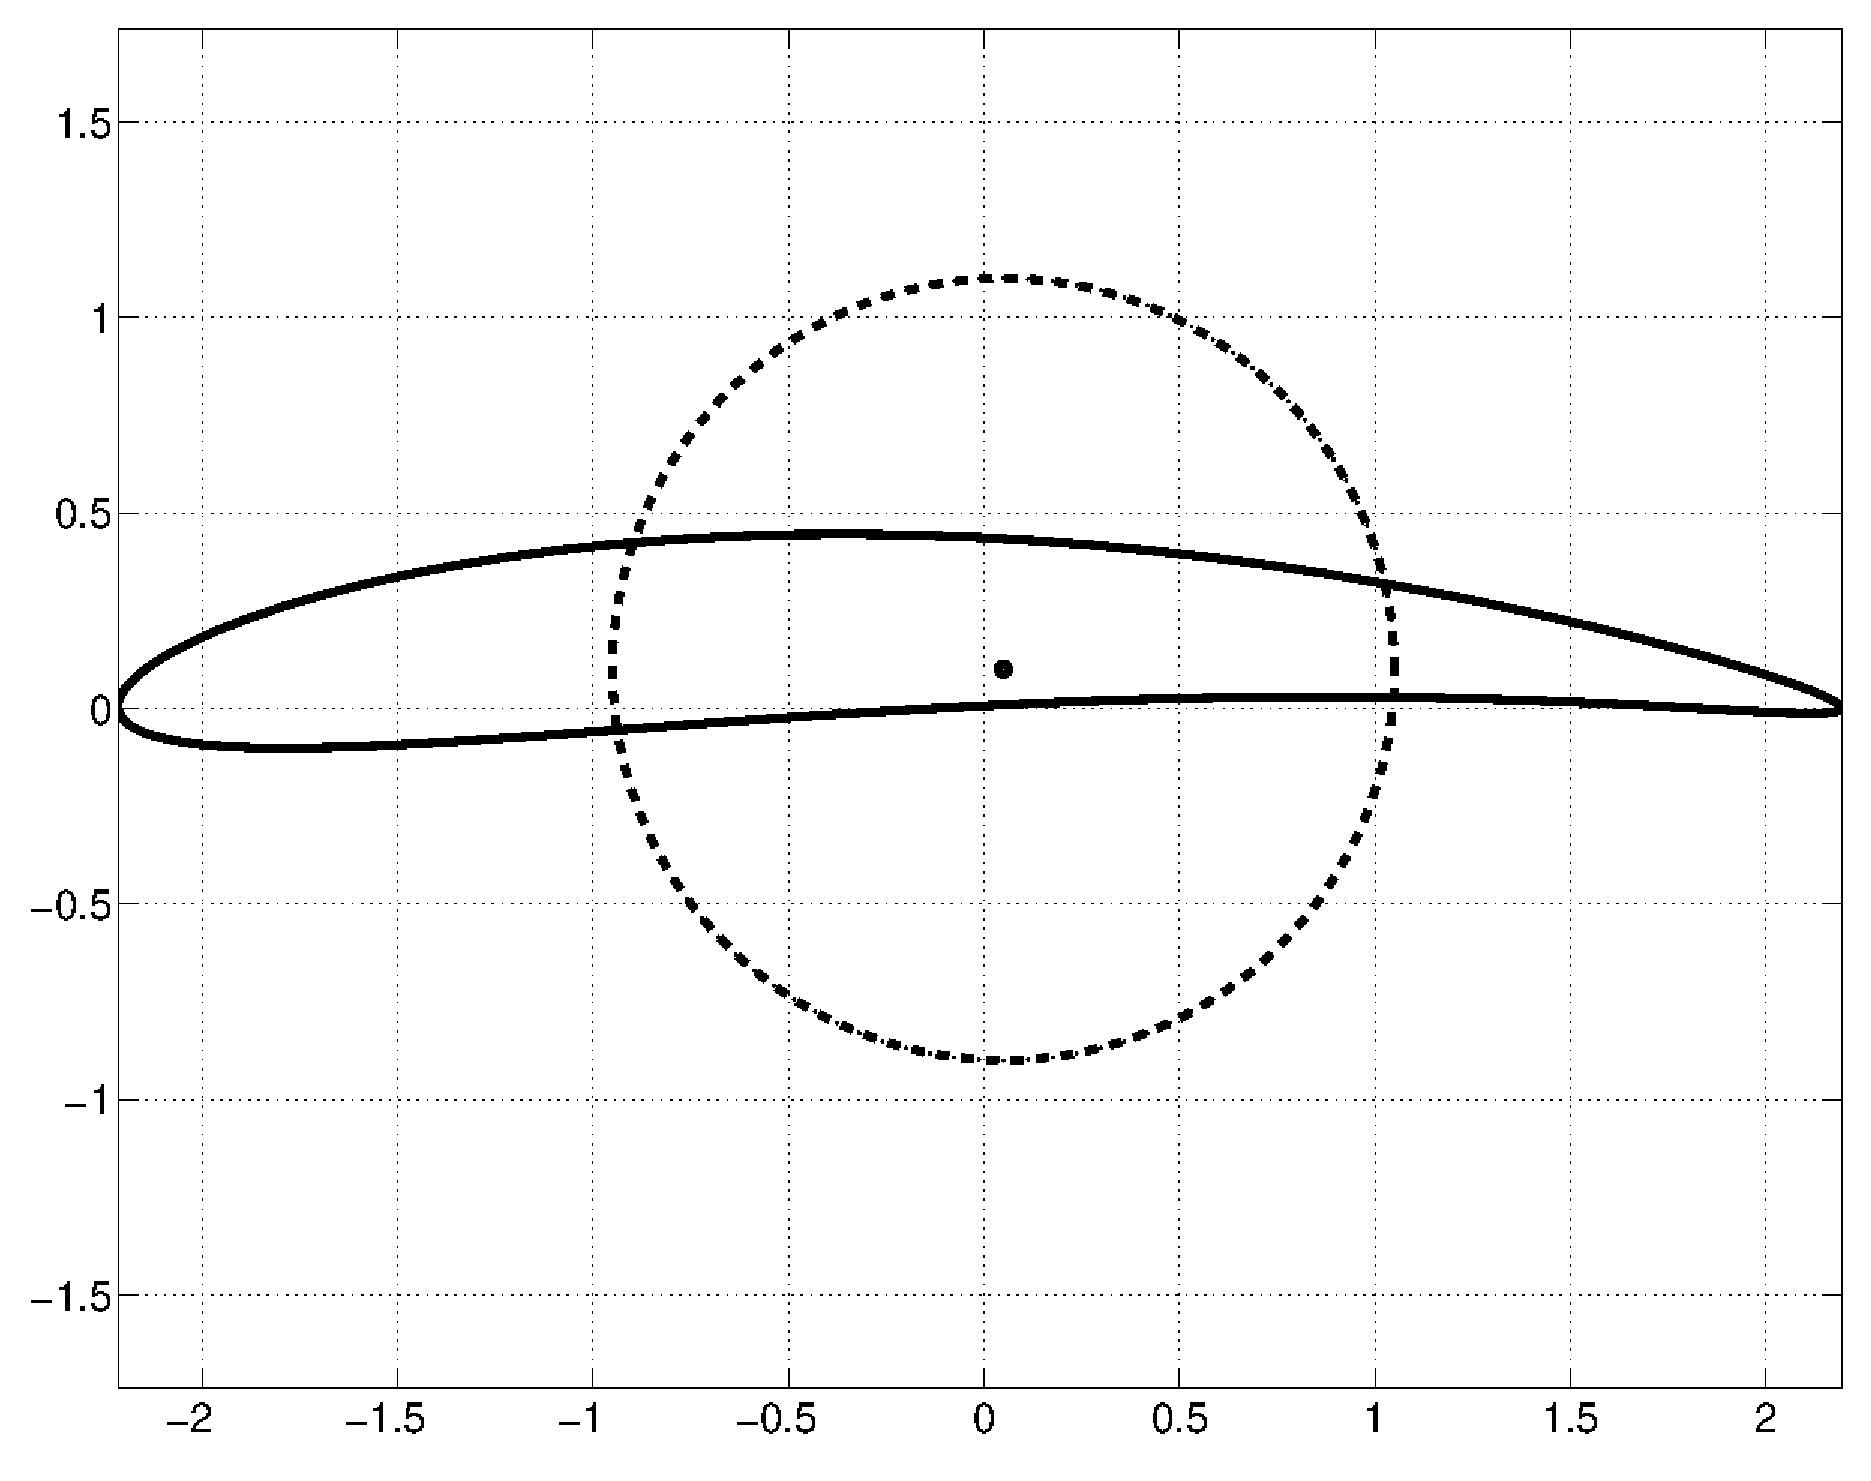
\includegraphics[width=4.25cm]{Chapter_5/figure/airfoil_camber.eps}
    }
    \quad
    \subfigure[$x_c = 0.1, y_c = 0.0$]
    {
    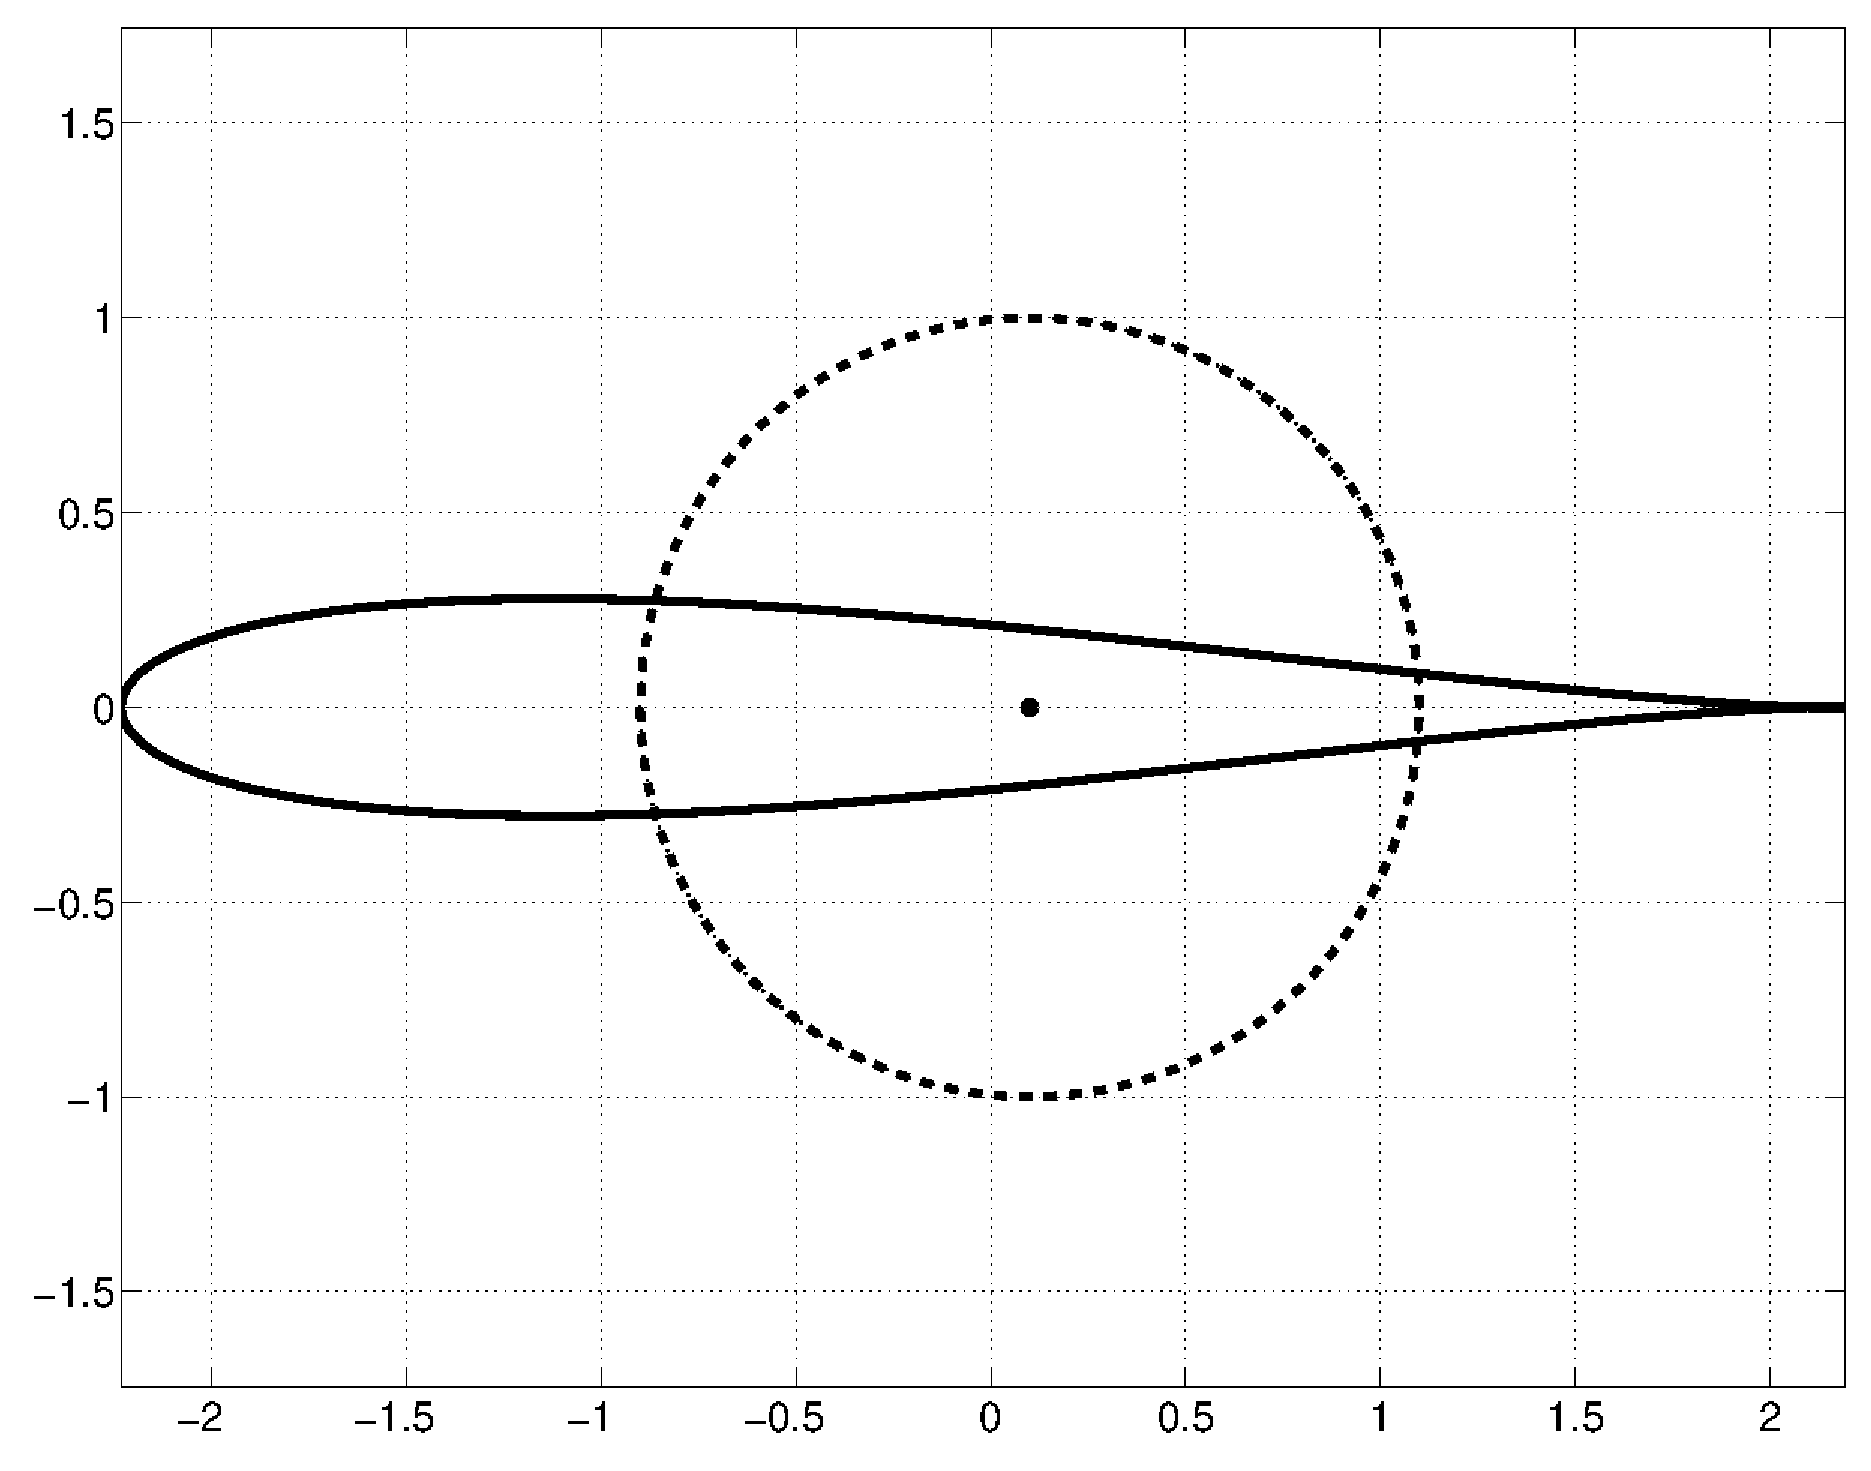
\includegraphics[width=4.25cm]{Chapter_5/figure/airfoil_thickness.eps}
    }
    \caption{Effect of circle location on Joukowsky airfoil shape.}
    \label{fig:C5_joukowskyAirfoil}
\end{figure}
%
The computational domain for this problem is defined as shown in Figure \ref{fig:C5_domainAirfoil}. The rigid airfoil is mounted on a two degree-of-freedom elastic structure as shown in Figure \ref{fig:C5_airfoilStructure}. The elastic structure contains axial and torsional springs to represent an actual wing more accurately.
%
\begin{figure}[H]
    \centering
    \subfigure[Physical domain.]
    {
    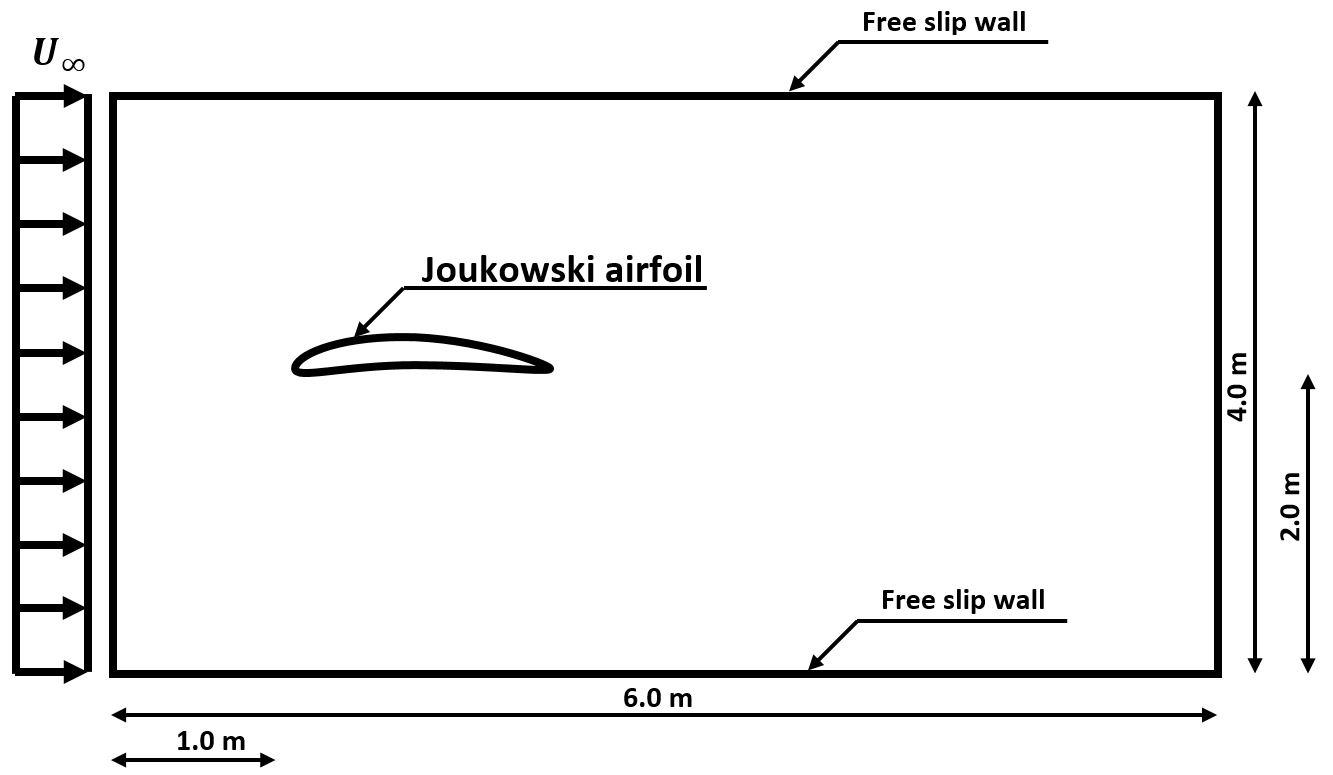
\includegraphics[width=8cm]{Chapter_5/figure/airfoilPhysicalDomain.JPG}
    \label{fig:C5_domainAirfoil}
    }
    \quad
    \subfigure[Airfoil elastic structure]
    {
    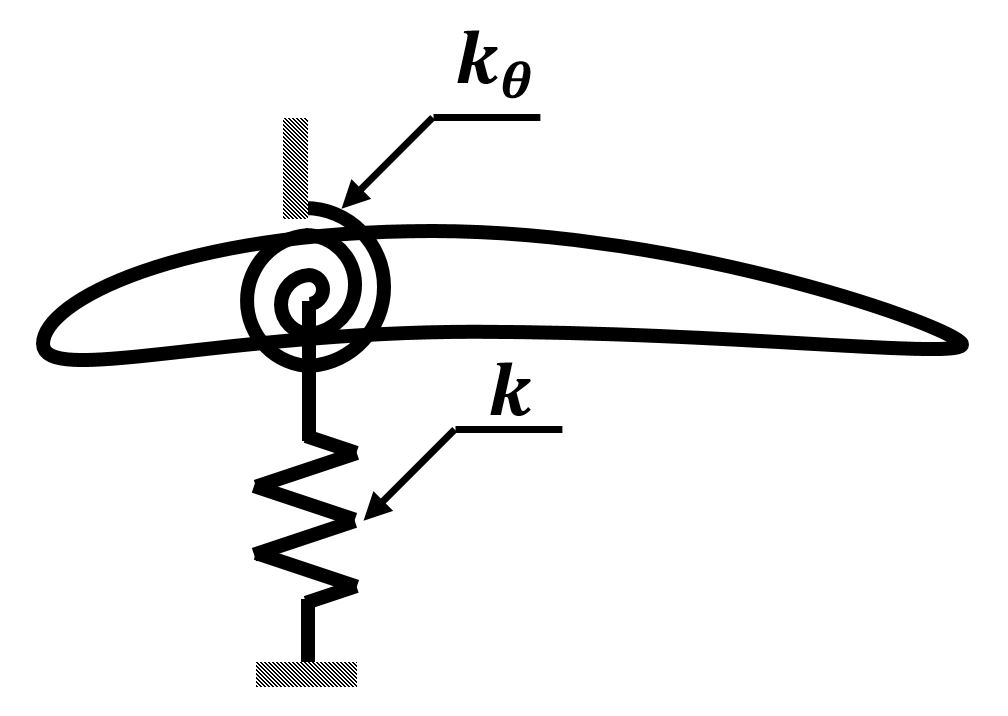
\includegraphics[width=5cm]{Chapter_5/figure/airfoilStructure.JPG}
    \label{fig:C5_airfoilStructure}
    }
    \caption{Physical domain and elastic structure for the pitching and plunging airfoil.}
\end{figure}
%
The governing equations for the elastic structure in the state-space form are shown in Equation \eqref{eq:C5_airfoilEquationOfMotion}.
%
\begin{equation}\label{eq:C5_airfoilEquationOfMotion}
\begin{bmatrix}
	\dot{y} \\
	\ddot{y} \\
	\dot{\theta} \\
	\ddot{\theta}
\end{bmatrix} = 
\begin{bmatrix}
	0 & 1 & 0 & 0 \\
	-\dfrac{k}{m} & 0 & 0 & 0 \\
	0 & 0 & 0 & 1 \\
	0 & 0 & -\dfrac{k_\theta}{I} & 0
\end{bmatrix}
\begin{bmatrix}
	y \\
	\dot{y} \\
	\theta \\
	\dot{\theta}
\end{bmatrix} + 
\begin{bmatrix}
	0 \\
	F \left( y, \dot{y}, t \right) \\
	0 \\
	M \left( \theta, \dot{\theta}, t \right)
\end{bmatrix}
\end{equation}
%
where $m$ is airfoil mass; $k$ is axial spring stiffness; $I$ is airfoil moment of inertia around its quarter-chord; $k_\theta$ is rotational spring stiffness; $F$ is the force in $y$ direction (lift generated by airfoil); and $M$ is the moment at quarter-chord. The force and moment are calculated using the pressure field from the solution of NS equations. Adams-bashforth method is used to explicitly integrate Equation \eqref{eq:C5_airfoilEquationOfMotion} in time.

For this problem, we look at two different airfoils mounted on the elastic structure as shown in Figure \ref{fig:C5_airfoilShape}. The difference in airfoil shape will result in different characteristics in the FSI response of the system. We refer to the airfoil defined in Figure \ref{fig:C5_thinAirfoil} as \emph{thin airfoil} and the one in Figure \ref{fig:C5_thickAirfoil} as \emph{thick airfoil}.
%
\begin{figure}[H]
    \centering
    \subfigure[$x_c = 0.05, y_c = 0.1$]
    {
    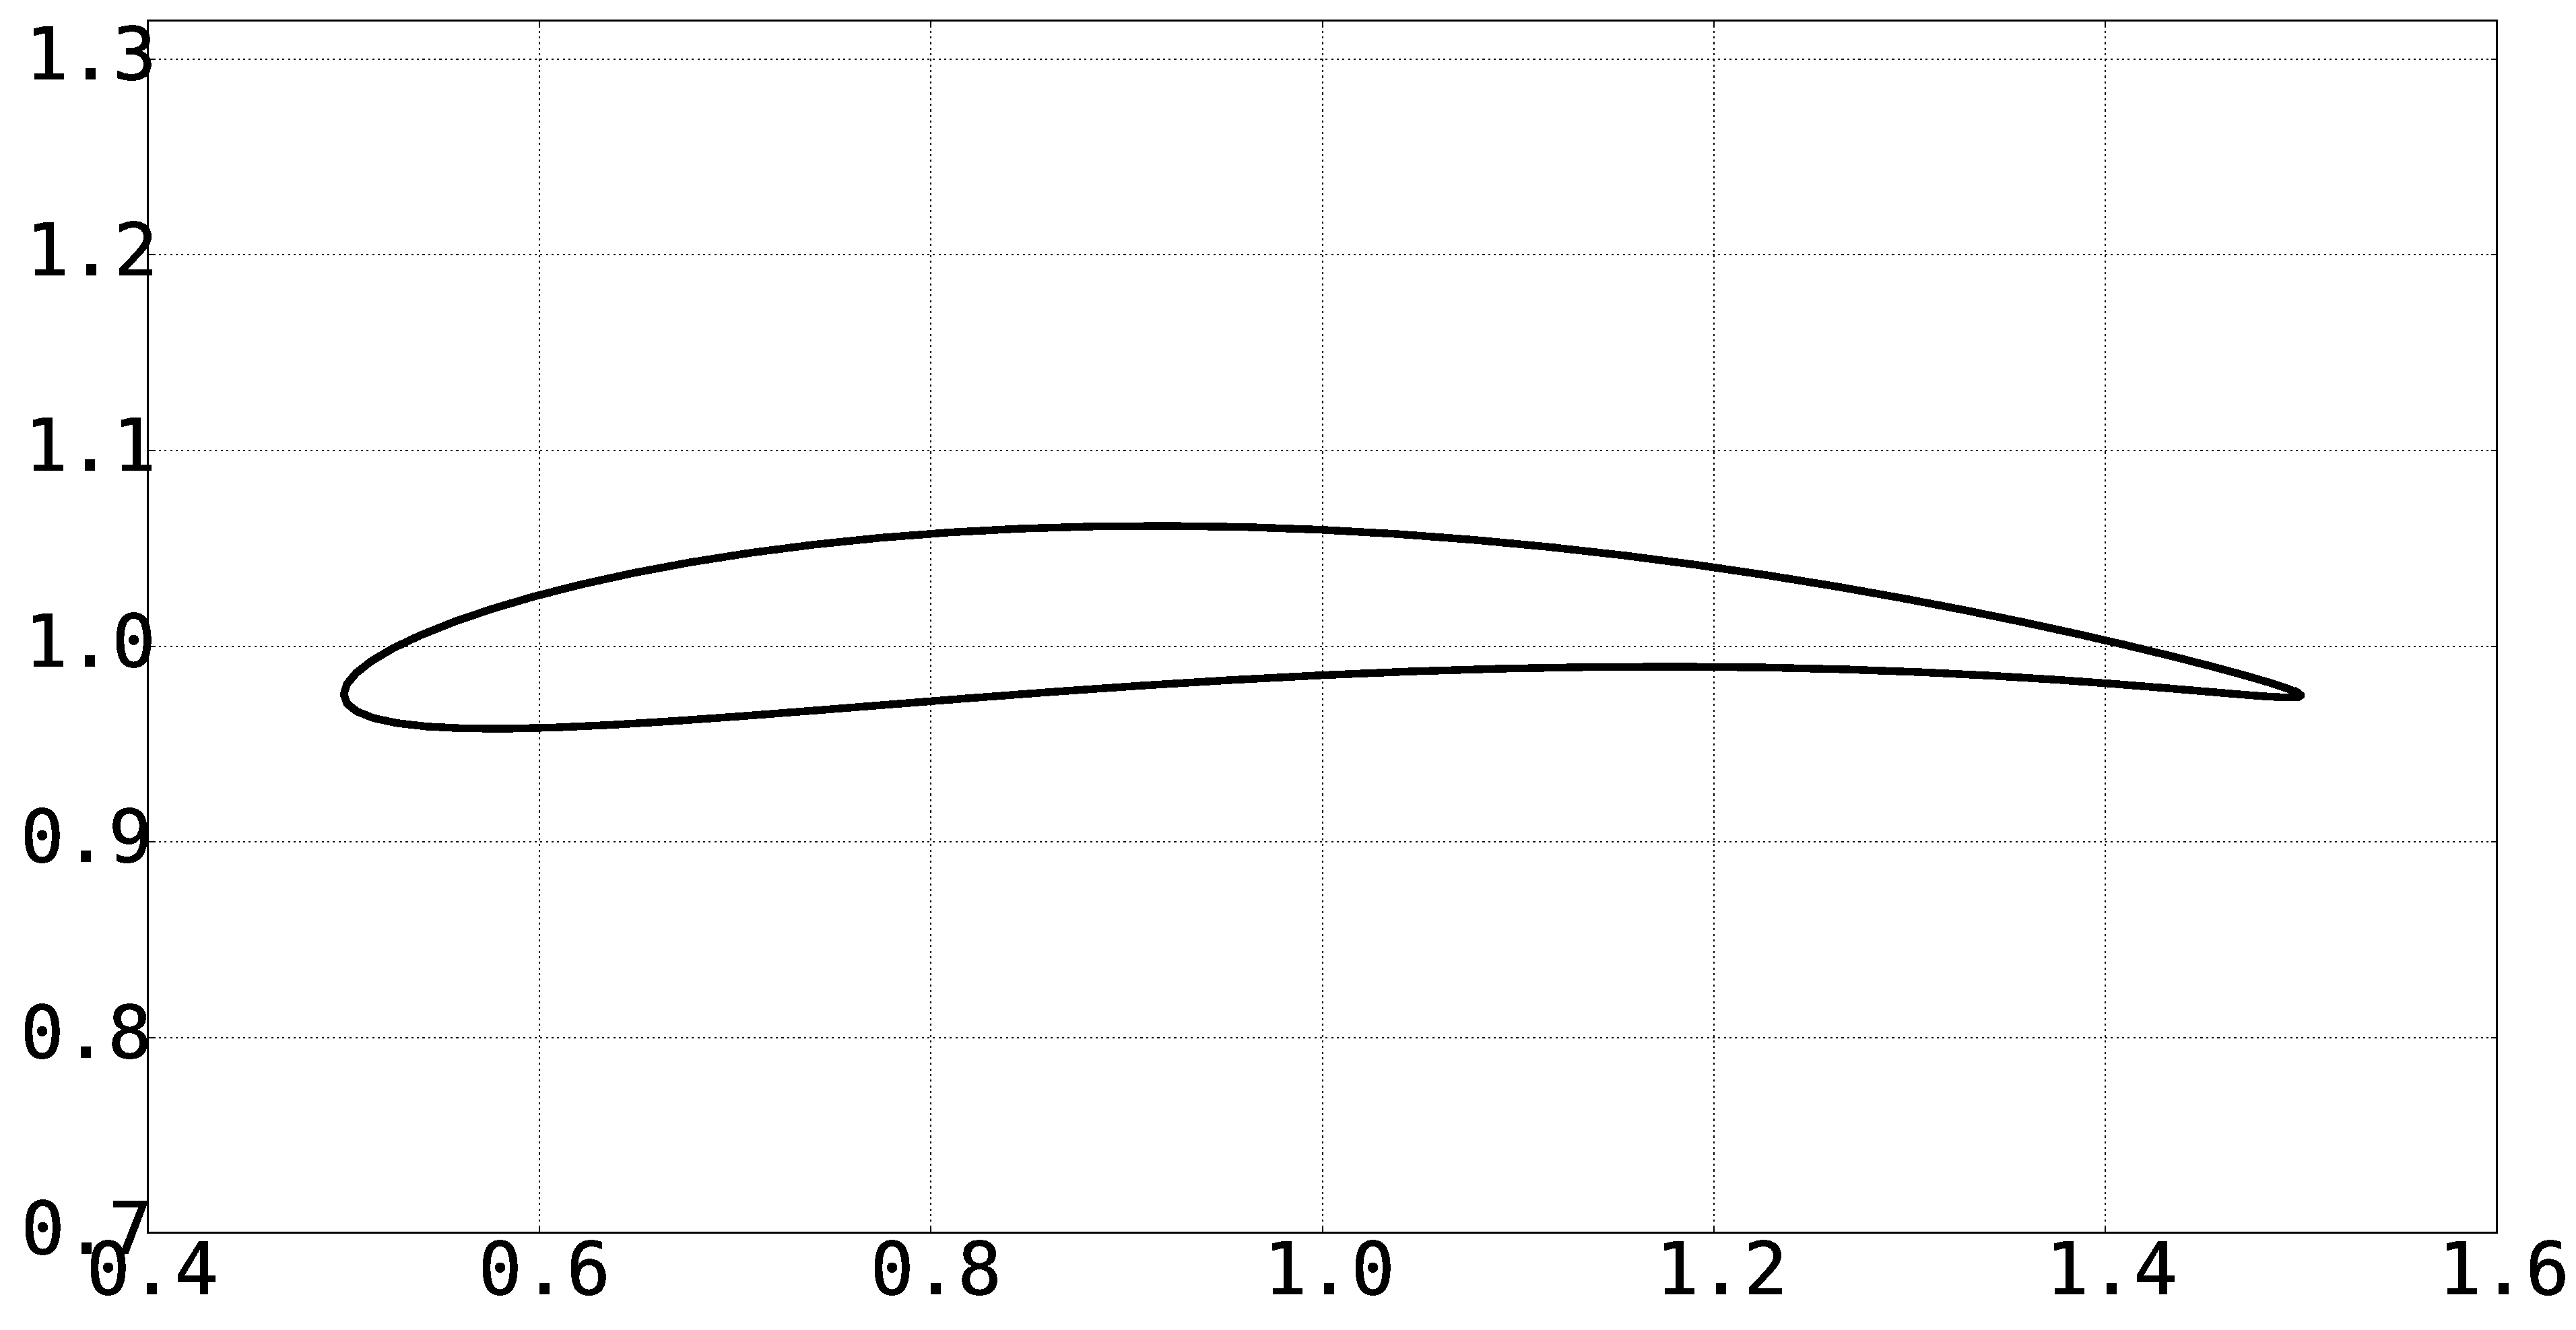
\includegraphics[width=6.5cm]{Chapter_5/figure/airfoil1.eps}
    \label{fig:C5_thinAirfoil}
    }
    \quad
    \subfigure[$x_c = 0.1, y_c = 0.2$]
    {
    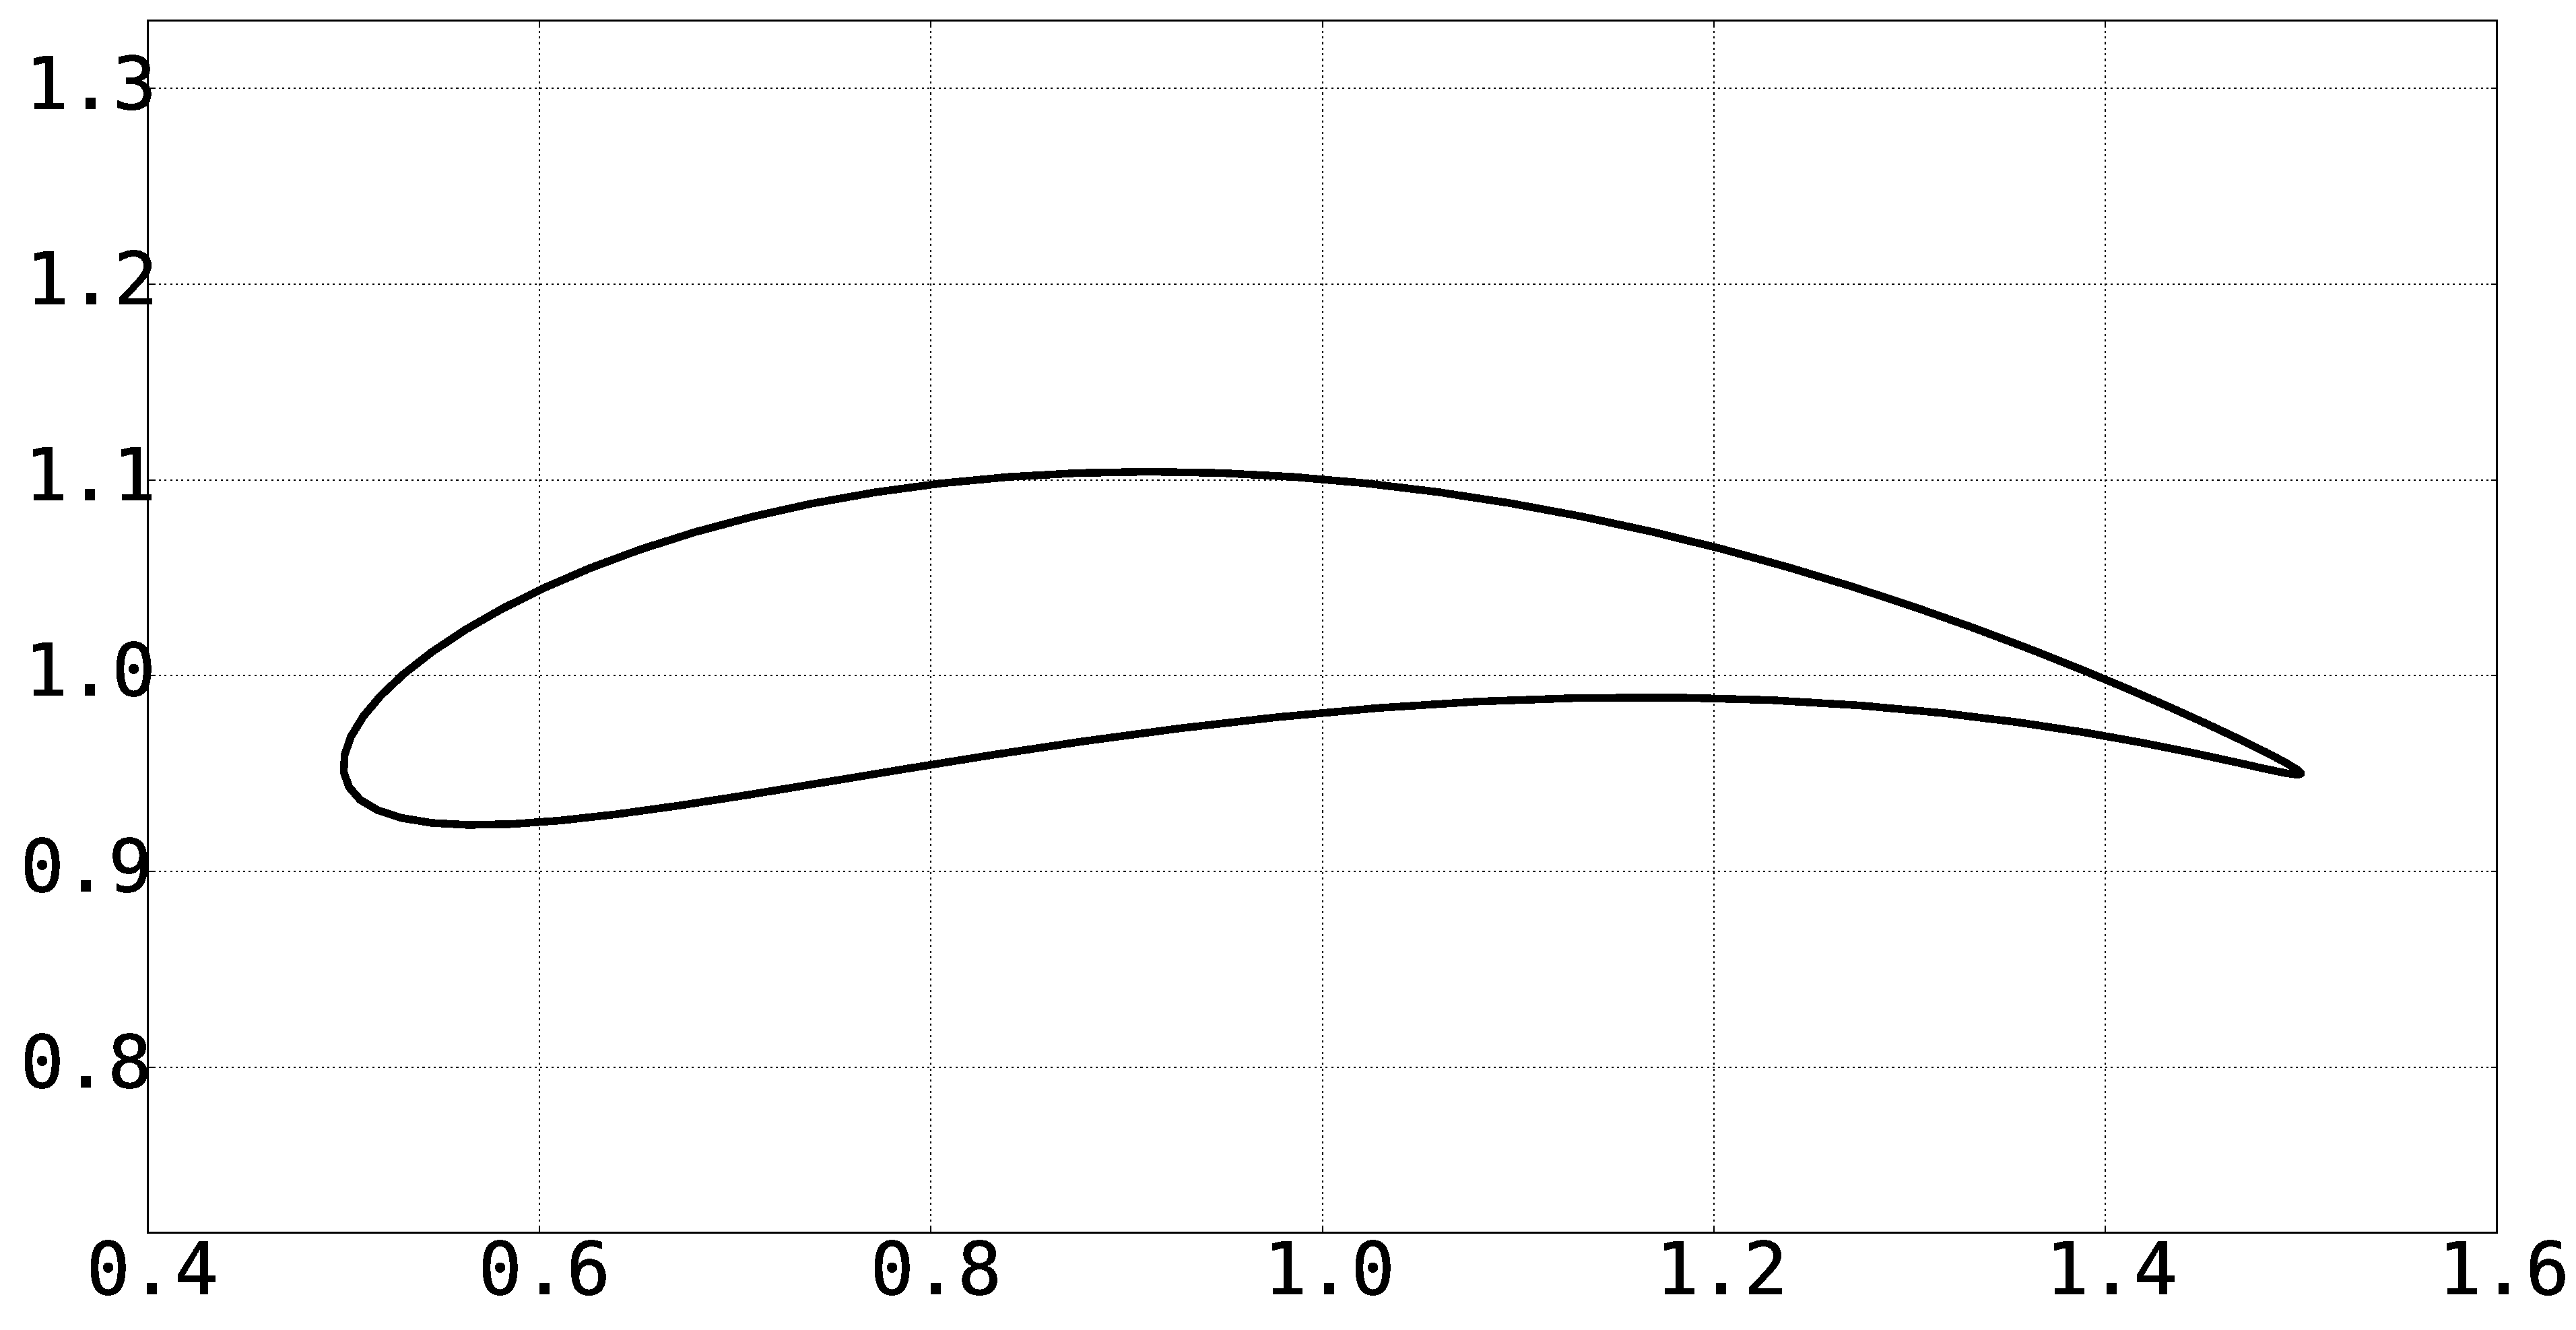
\includegraphics[width=6.5cm]{Chapter_5/figure/airfoil2.eps}
    \label{fig:C5_thickAirfoil}
    }
    \caption{Airfoil shape used for FSI calculation.}
    \label{fig:C5_airfoilShape}
\end{figure}
%
The Reynolds number for this simulation is selected as $100$. At higher Reynolds number will result in turbulent flow which is not the subject of this research. For the elastic structure properties, spring stiffness is selected as $0.5 N/m$, airfoil mass as $1.0 Kg$, rotational spring as $0.1 N/\theta$, and the moment of inertia as $1.0 Kg \cdot m^2$. The results of the first 50-second simulation of the airfoil center location and change in the angle of attack due to aerodynamic loads are shown in Figure \ref{fig:C5_airfoilDisplacementRotation}. As shown here, the thin airfoil of Figure \ref{fig:C5_thinAirfoil} follows an oscillatory response whereas the thick airfoil of Figure \ref{fig:C5_thickAirfoil} experiences divergence.
%
\begin{figure}[H]
    \centering
    \subfigure[Thin airfoil displacement]
    {
    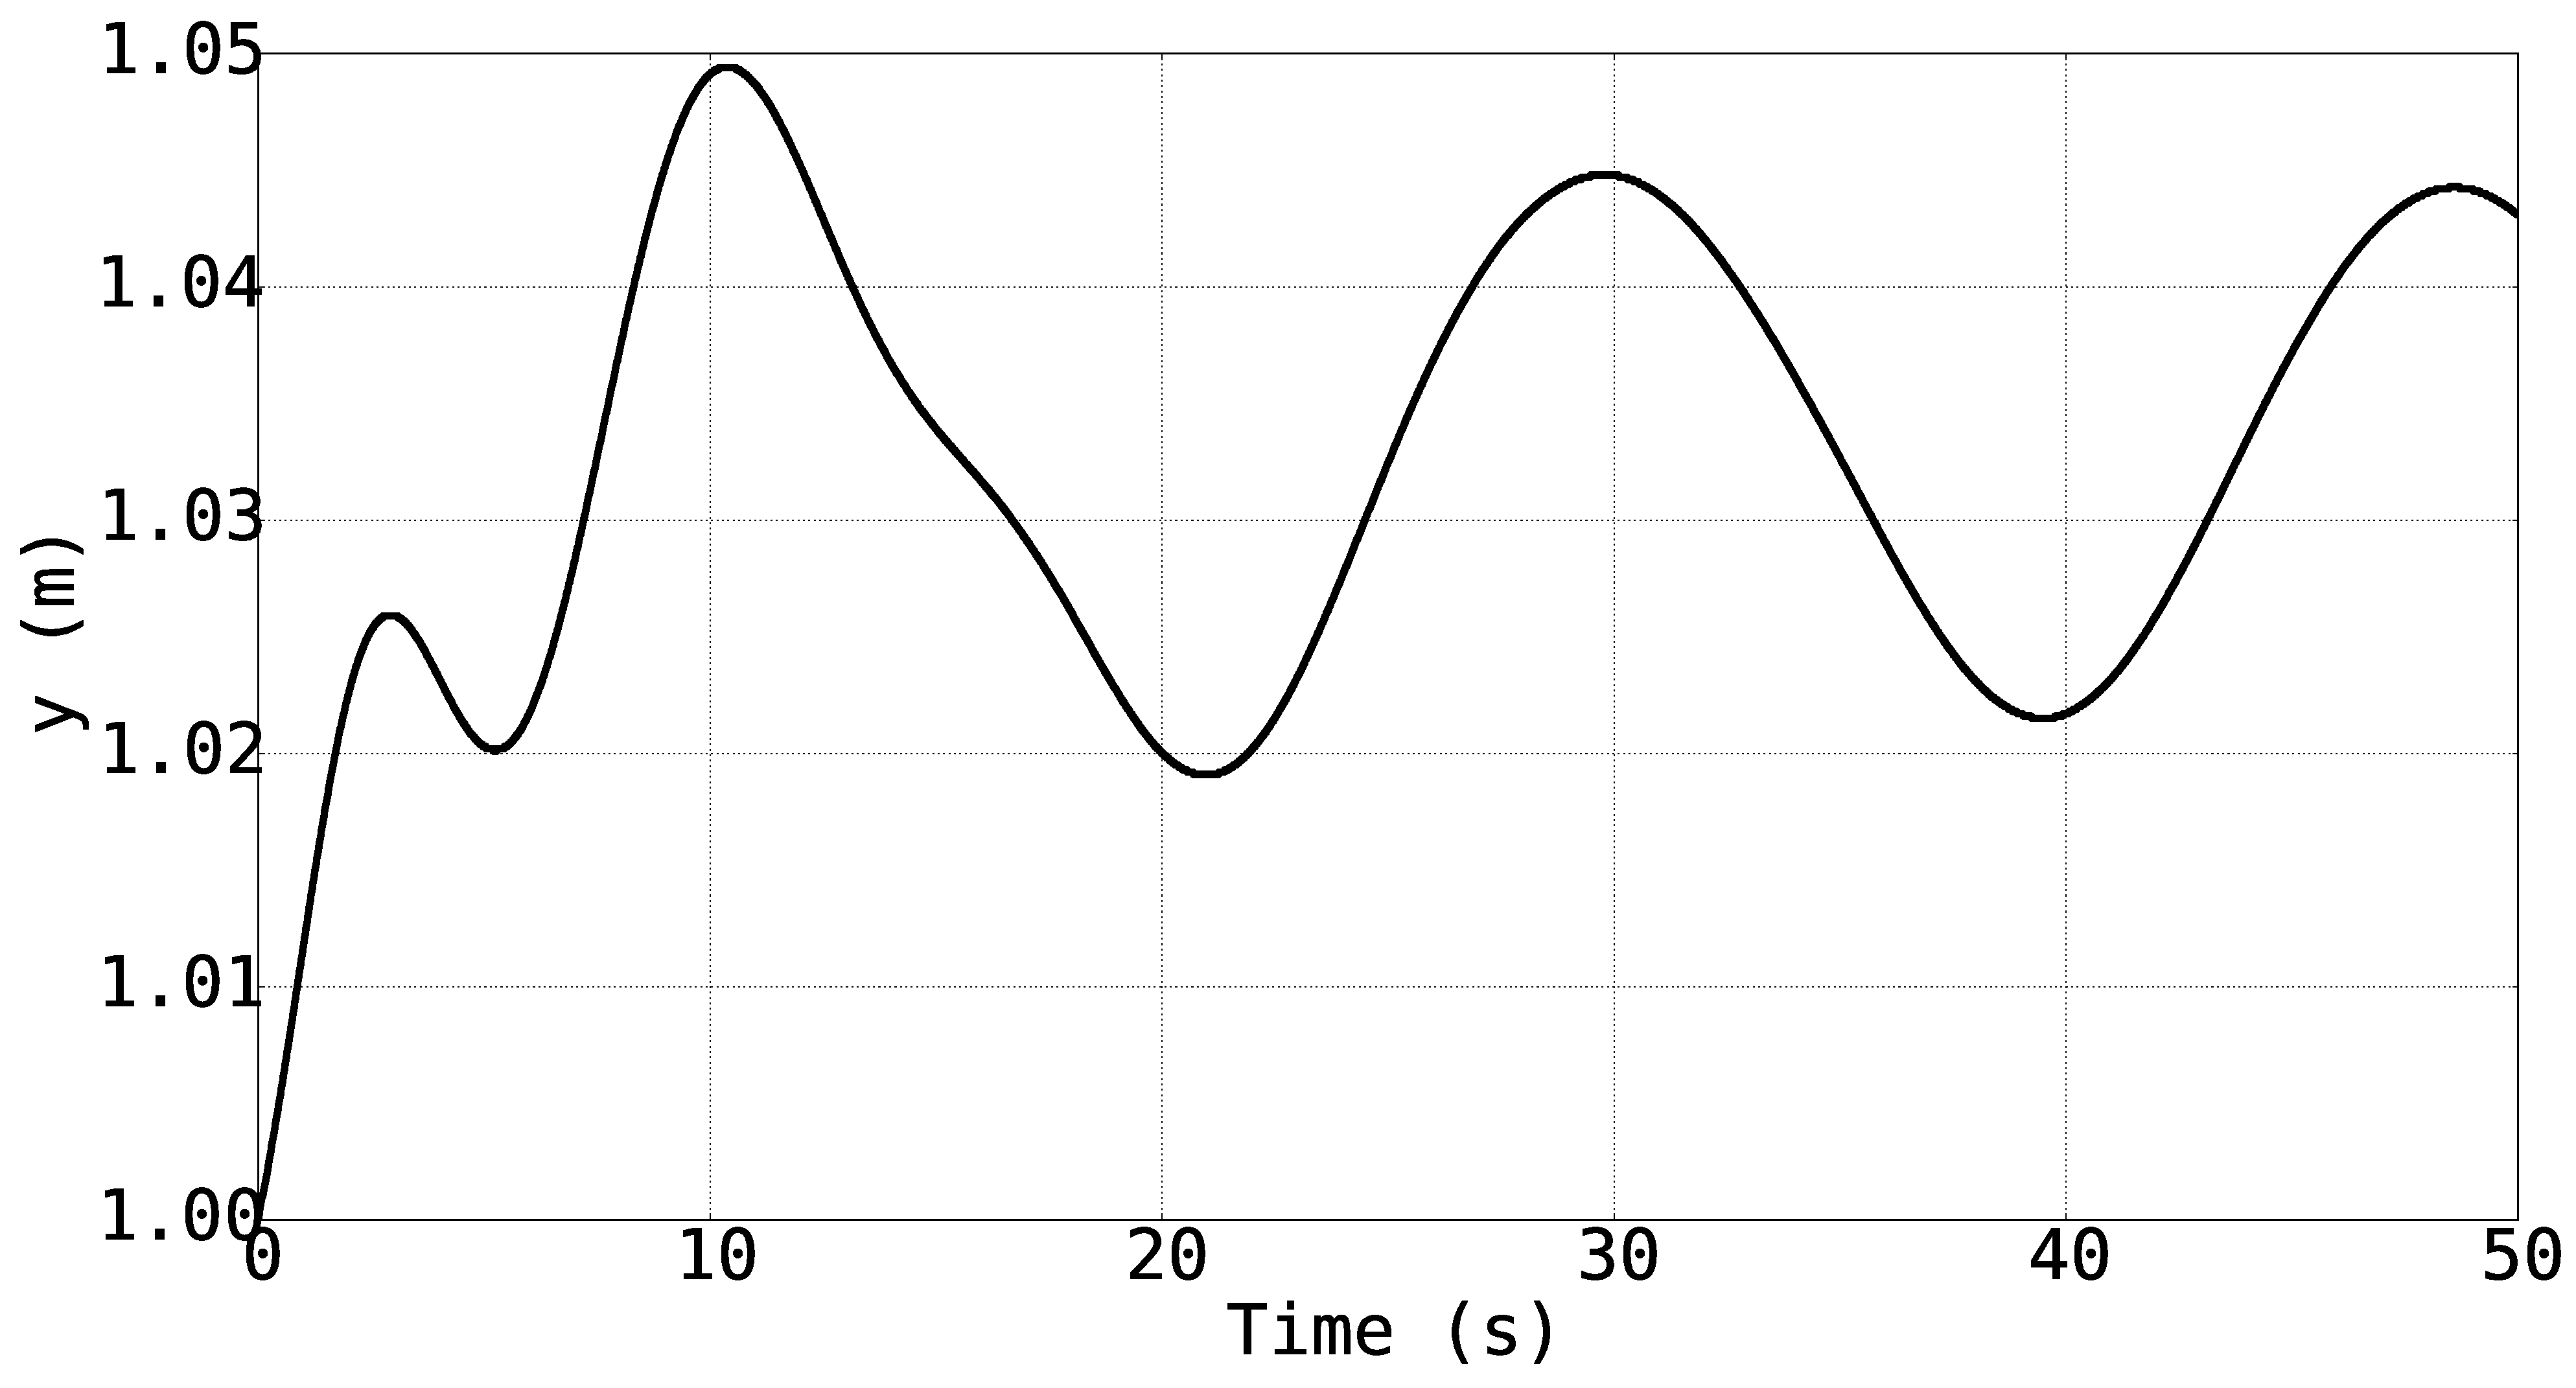
\includegraphics[width=6.5cm]{Chapter_5/figure/airfoil1_displacement.eps}
    }
    \quad
    \subfigure[Thick airfoil displacement]
    {
    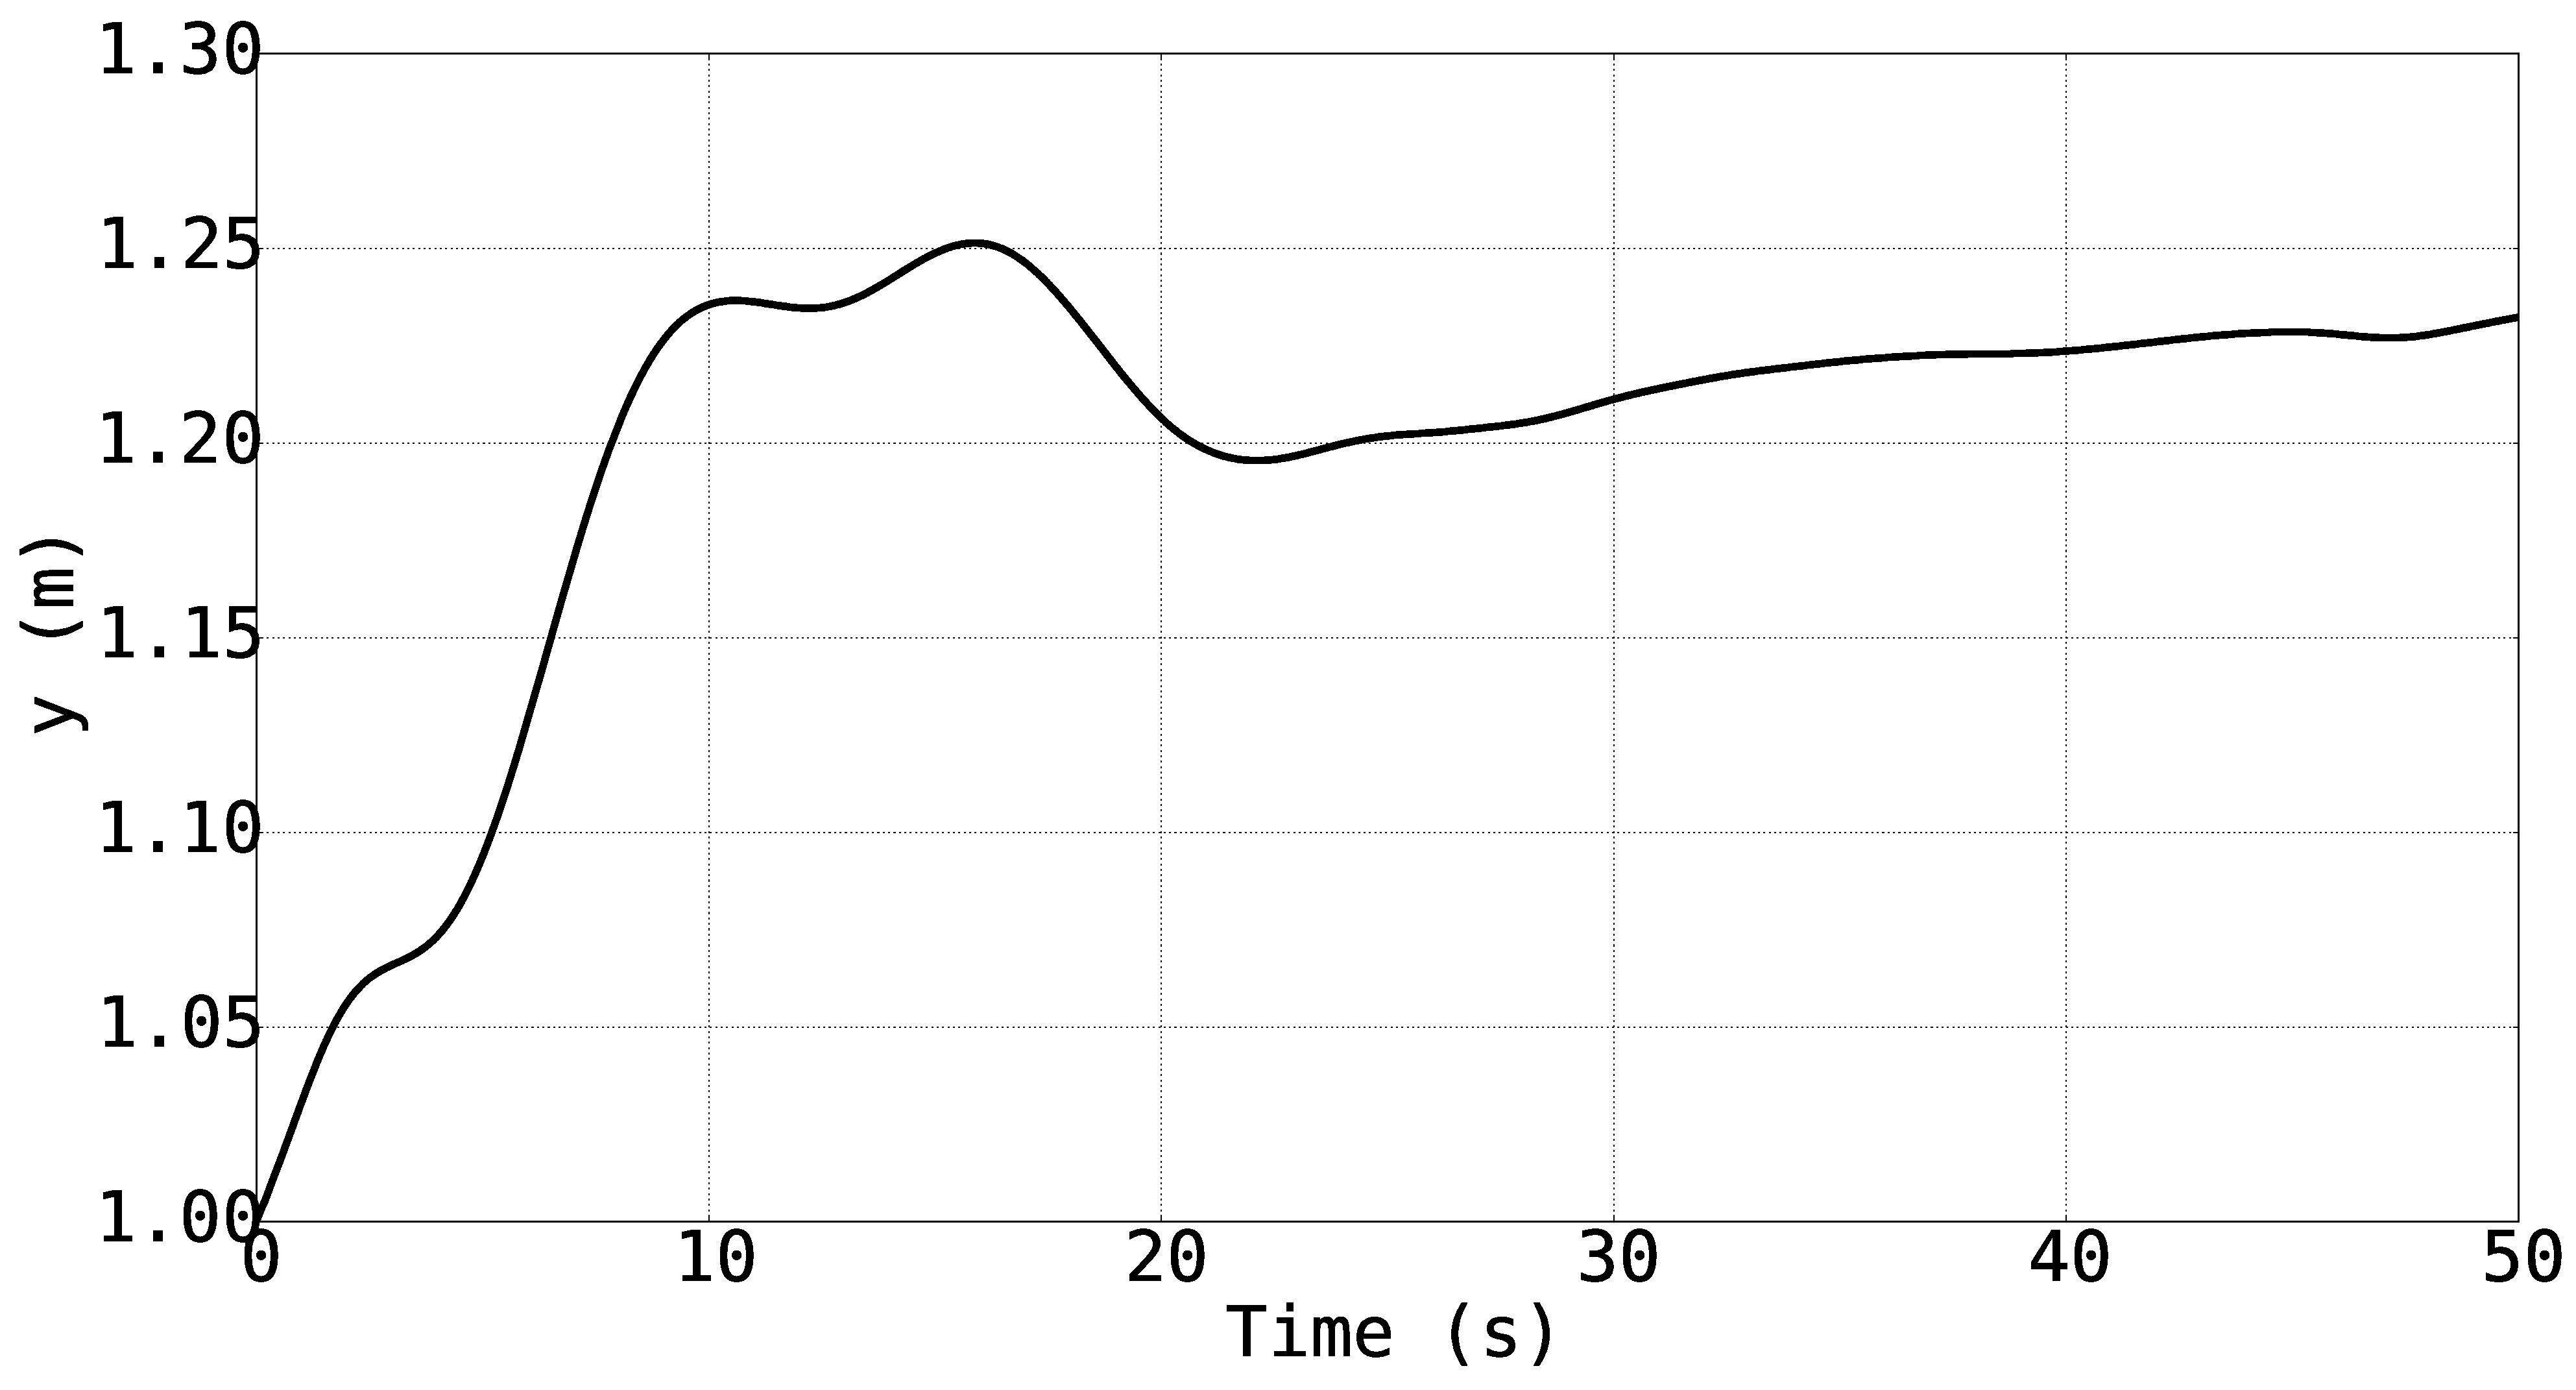
\includegraphics[width=6.5cm]{Chapter_5/figure/airfoil2_displacement.eps}
    }
    \\
    \subfigure[Thin airfoil rotation]
    {
    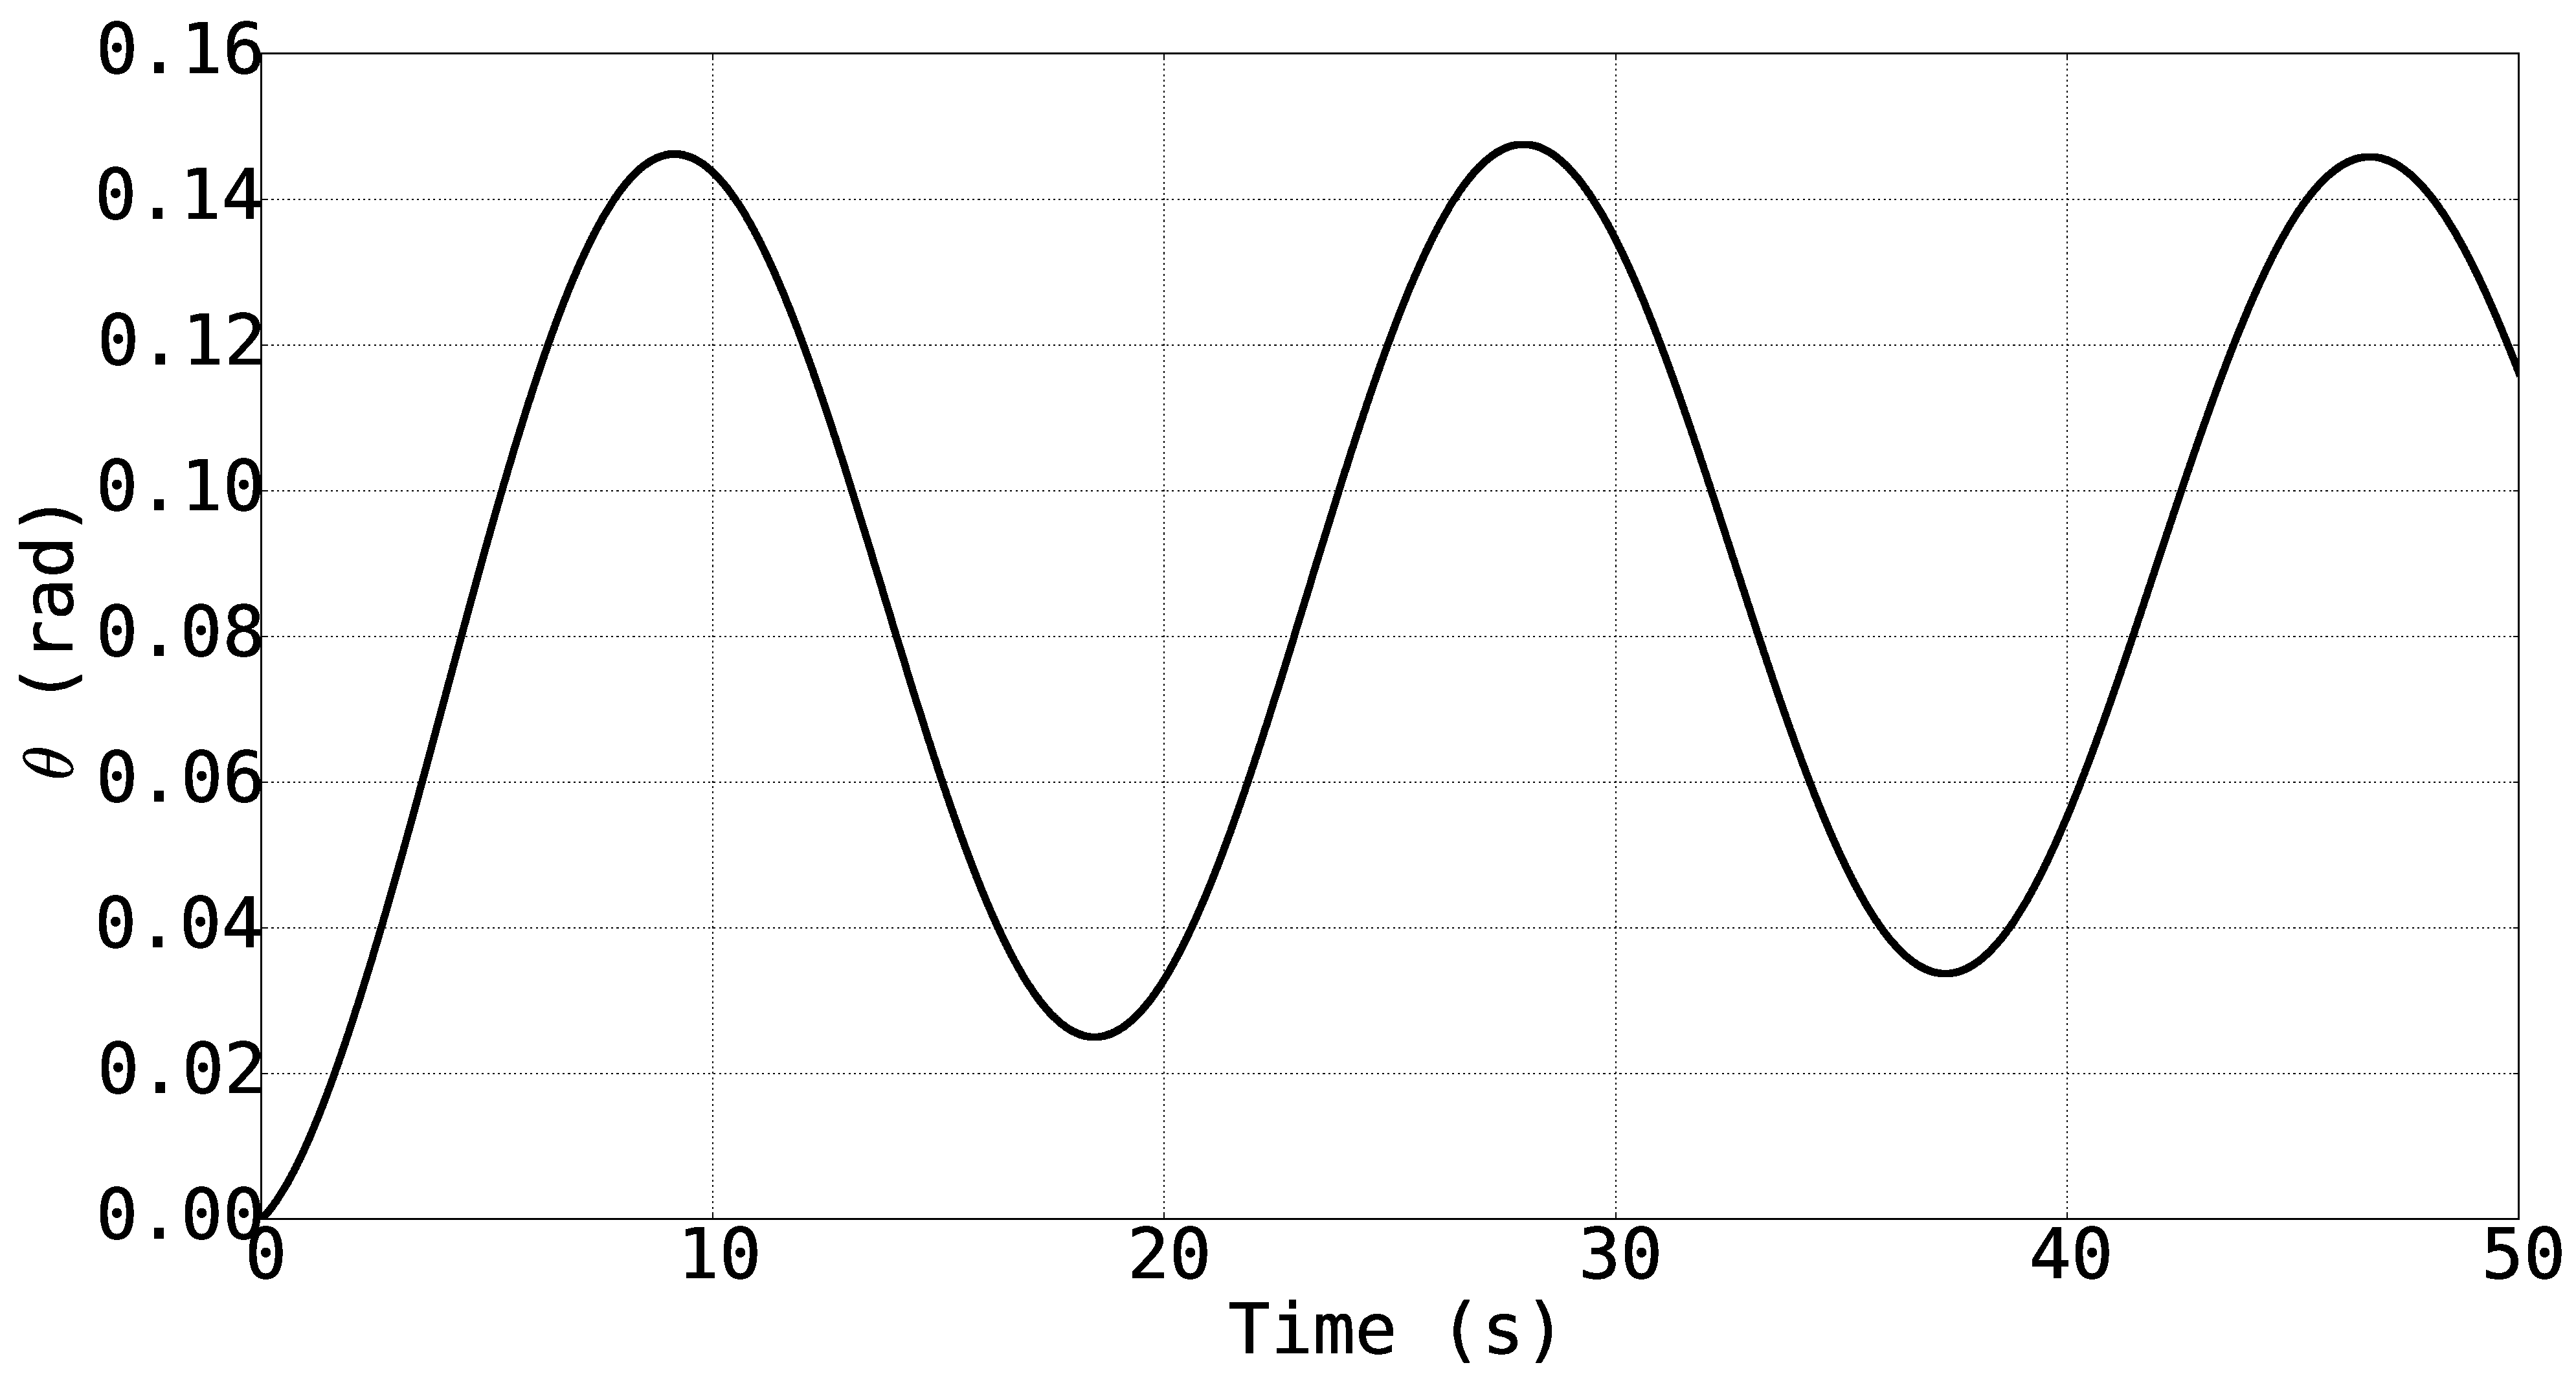
\includegraphics[width=6.5cm]{Chapter_5/figure/airfoil1_rotation.eps}
    }
    \quad
    \subfigure[Thick airfoil rotation]
    {
    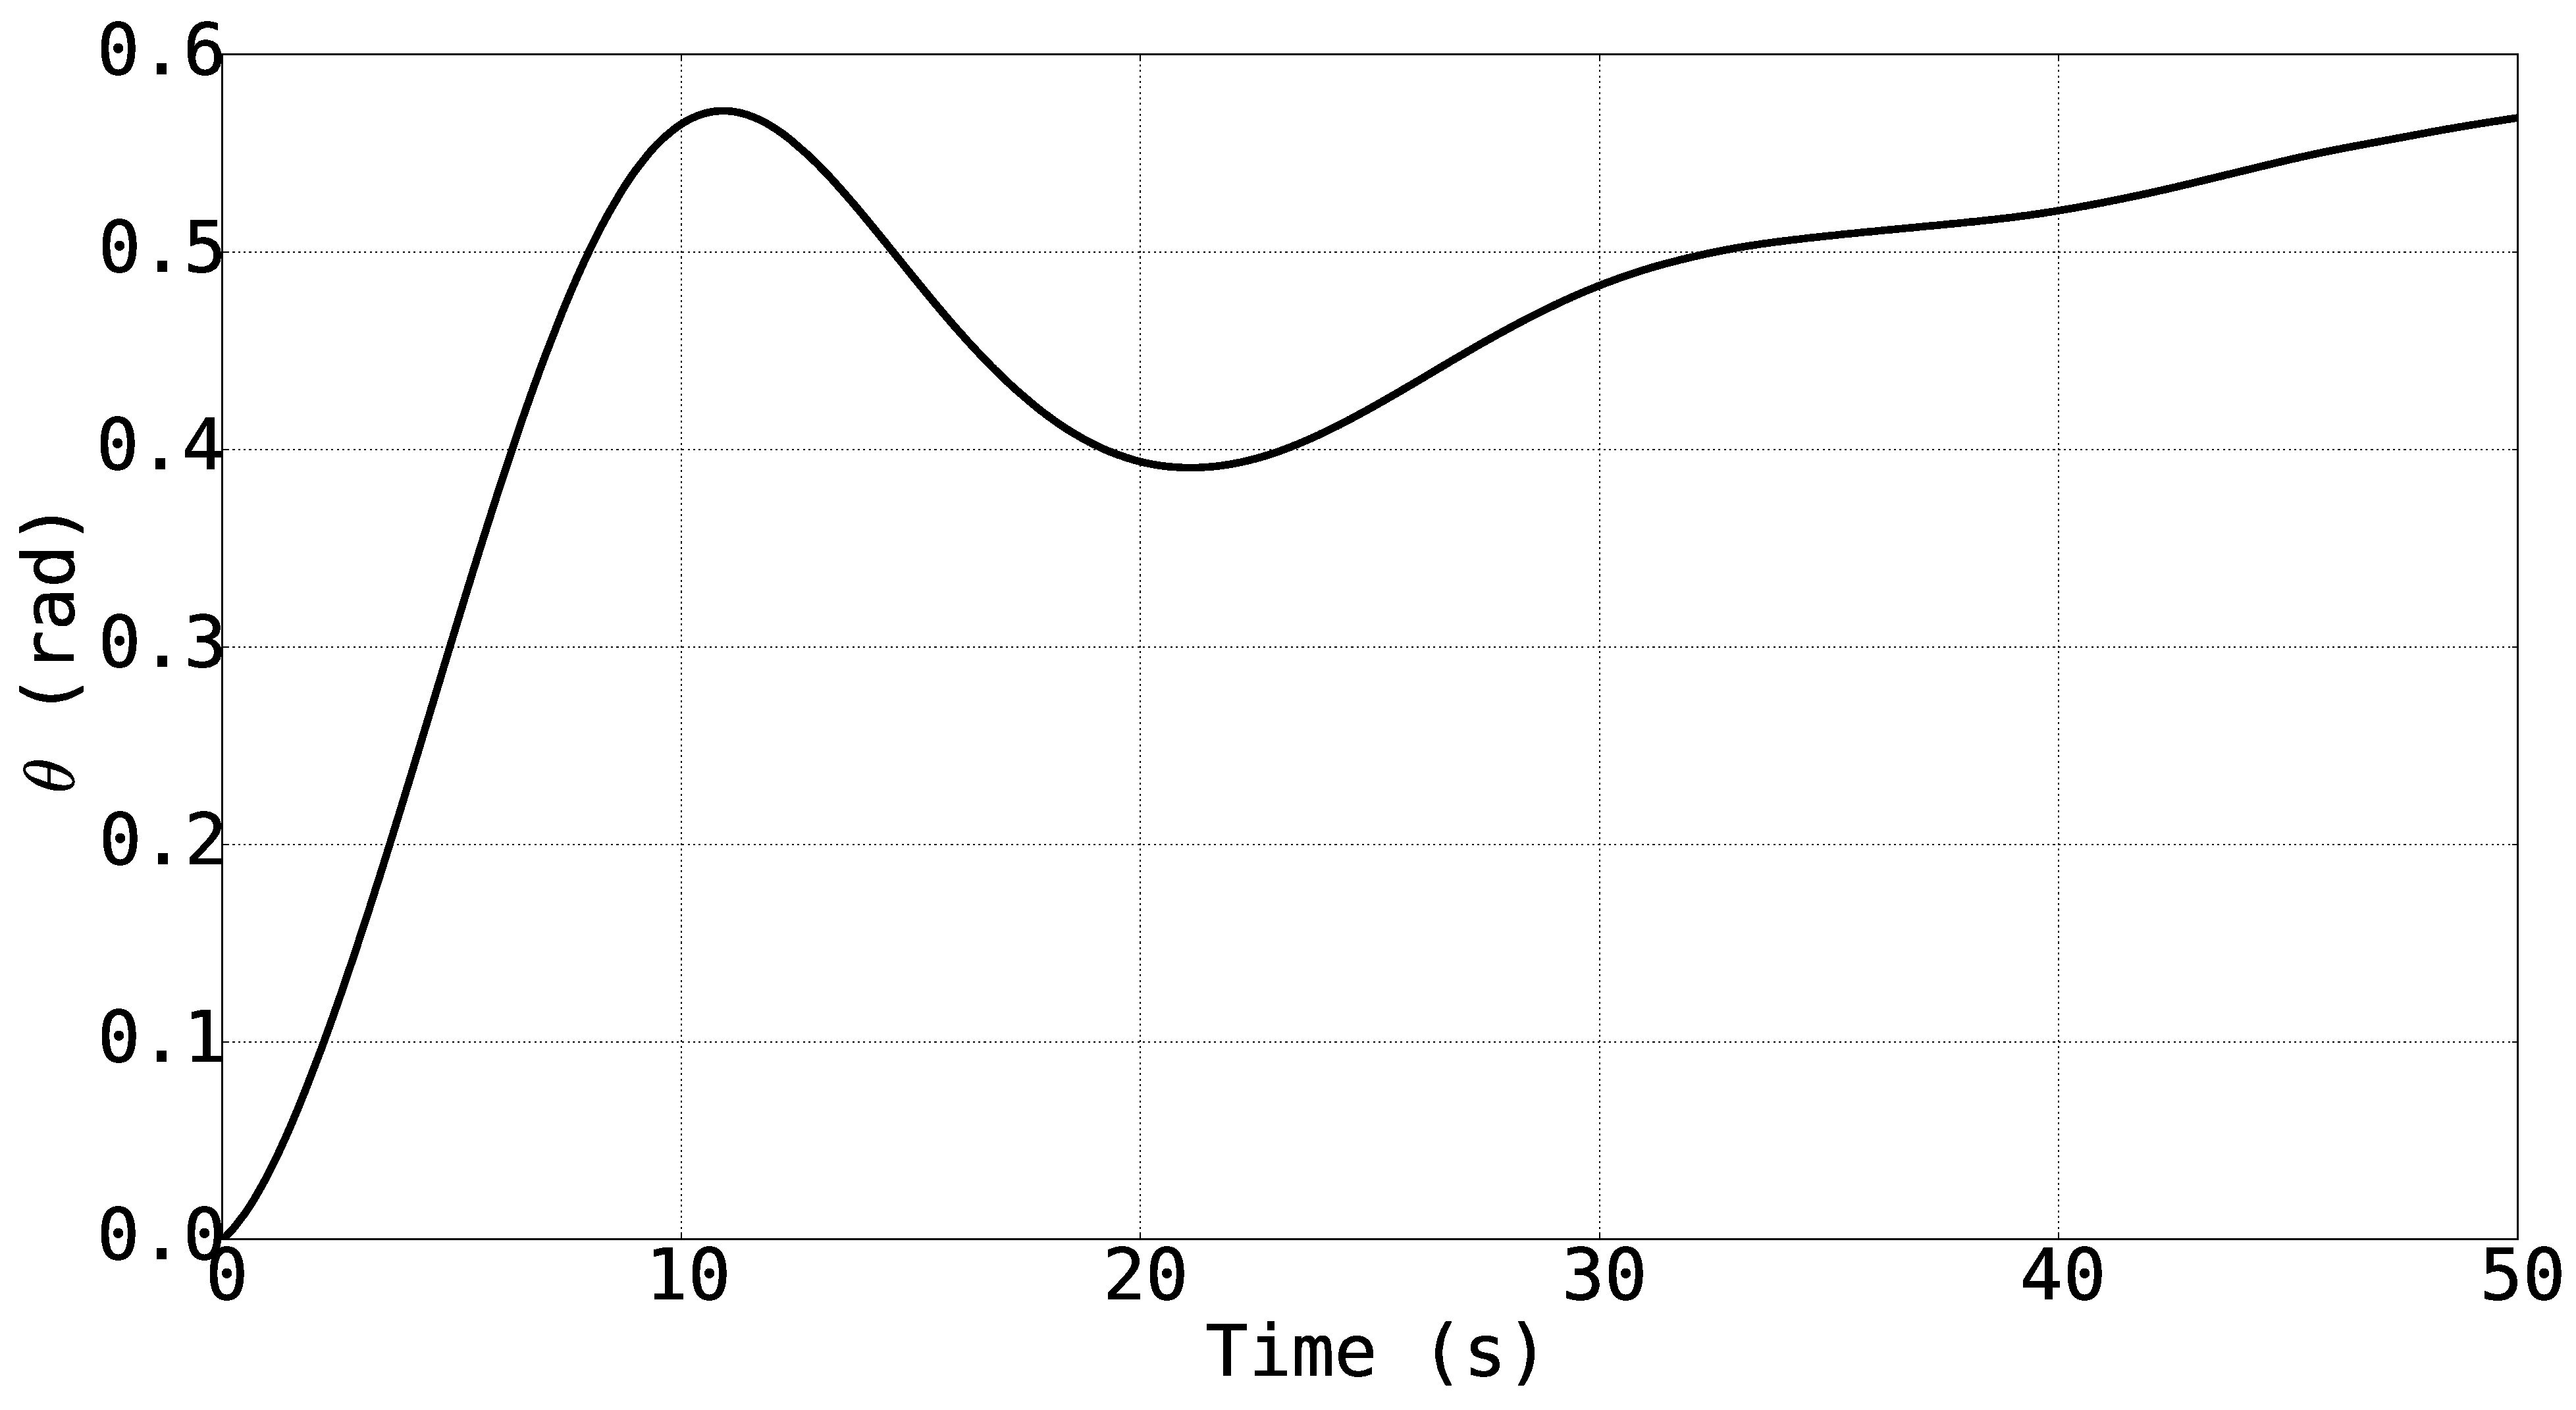
\includegraphics[width=6.5cm]{Chapter_5/figure/airfoil2_rotation.eps}
    }
    \caption{Airfoil displacement and rotation results due to aerodynamic loads.}
    \label{fig:C5_airfoilDisplacementRotation}
\end{figure}
%
To better understand the solution history, three snapshots from the u-velocity contour of the two airfoils are shown in Figure \ref{fig:C5_snapshotAirfoilSolution}. As shown here, the thick airfoil goes through large displacement and deformation. This is difficult to capture using the conventional body-conformal method; however, it can be done with rather ease by utilizing the current IB approach.
%
\begin{figure}[H]
    \centering
    \subfigure[$t = 0 \text{ sec}$]
    {
    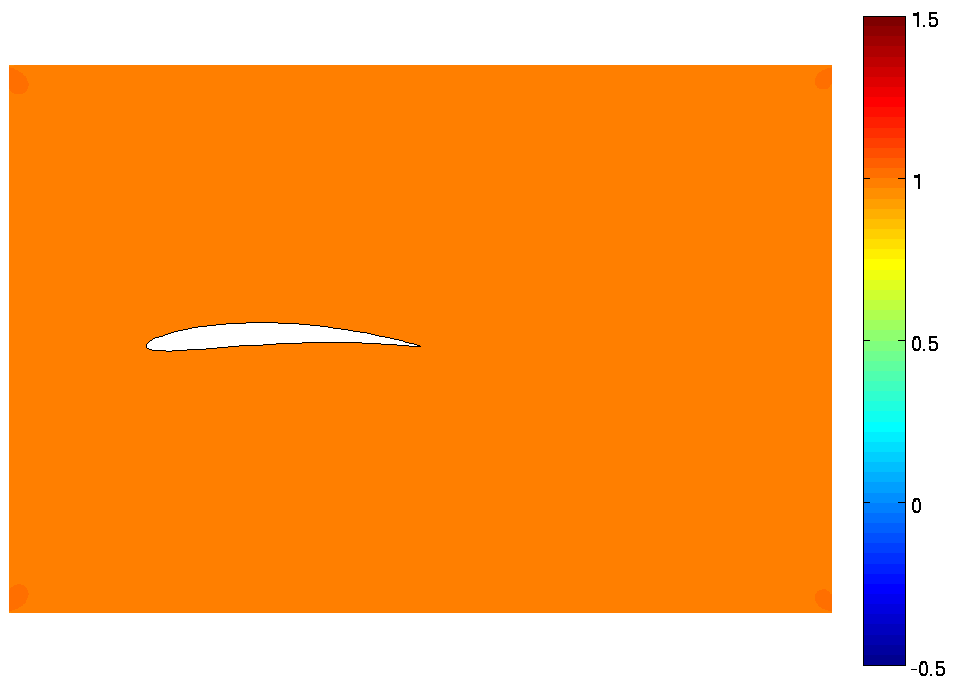
\includegraphics[width=4.25cm]{Chapter_5/figure/airfoil1_analysis_t0.png}
    }
    \quad
    \subfigure[$t = 5 \text{ sec}$]
    {
    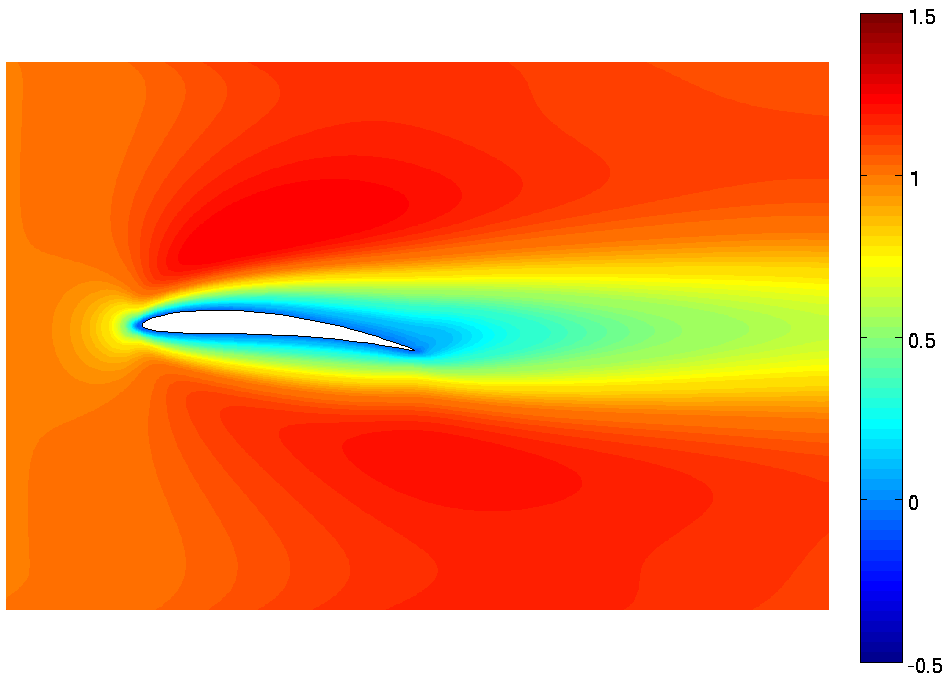
\includegraphics[width=4.25cm]{Chapter_5/figure/airfoil1_analysis_t5.png}
    }
    \quad
    \subfigure[$t = 25 \text{ sec}$]
    {
    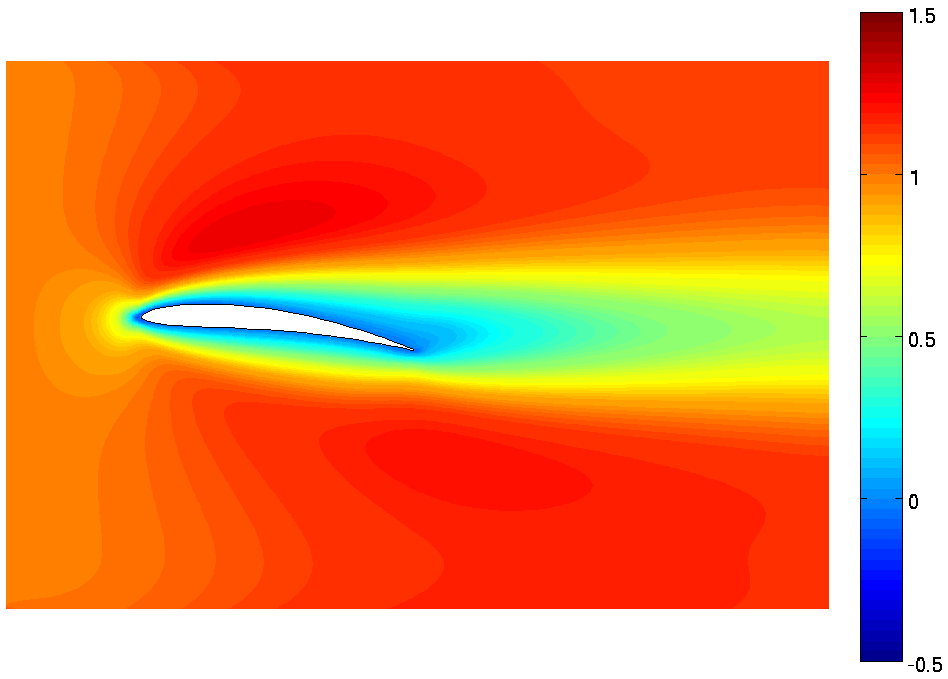
\includegraphics[width=4.25cm]{Chapter_5/figure/airfoil1_analysis_t25.png}
    }
    \\
    \subfigure[$t = 0 \text{ sec}$]
    {
    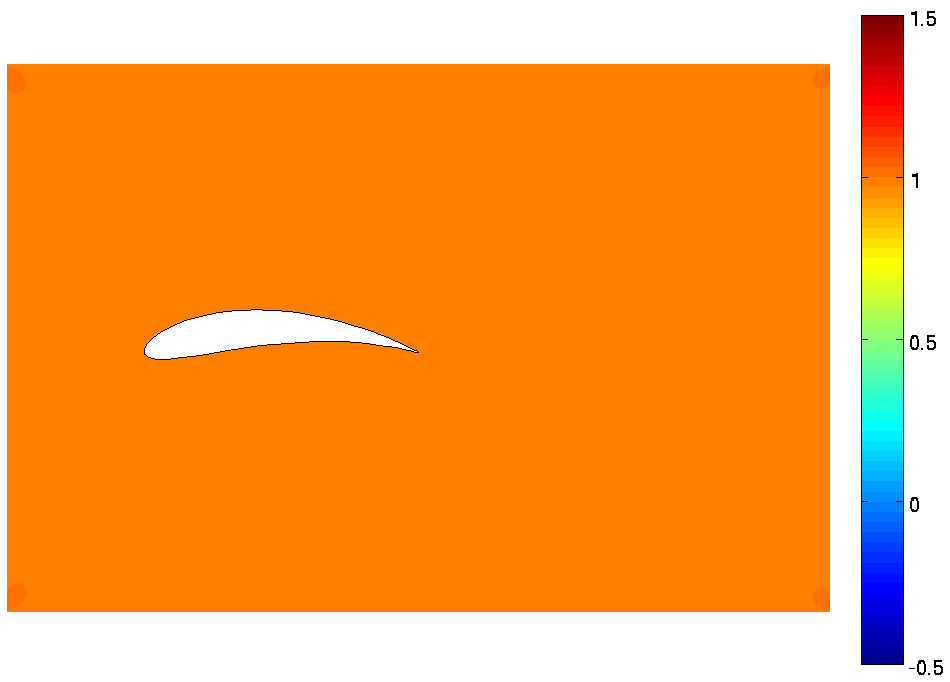
\includegraphics[width=4.25cm]{Chapter_5/figure/airfoil2_analysis_t0.png}
    }
    \quad
    \subfigure[$t = 5 \text{ sec}$]
    {
    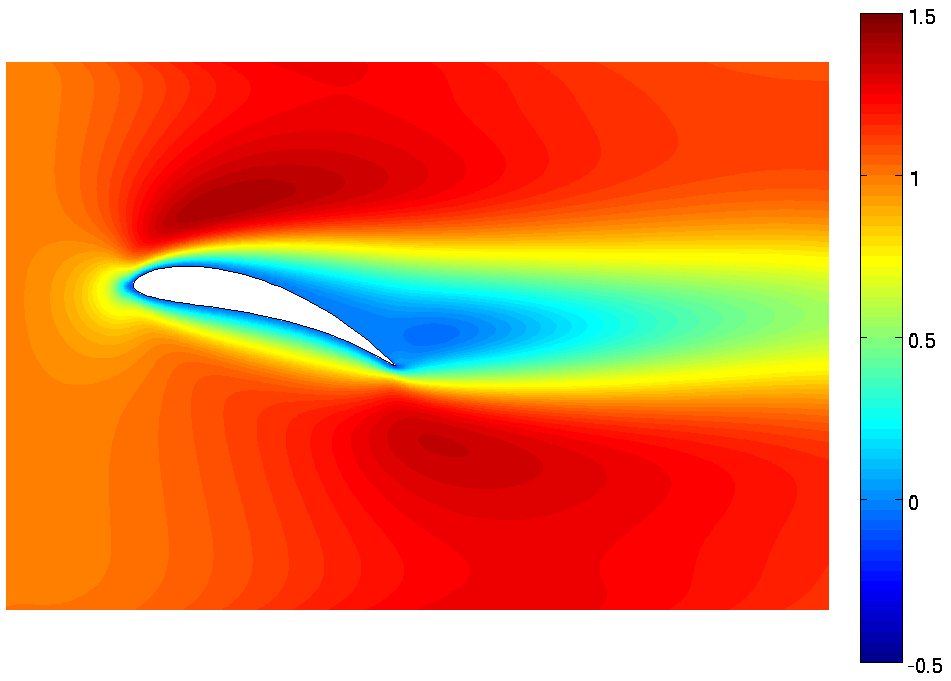
\includegraphics[width=4.25cm]{Chapter_5/figure/airfoil2_analysis_t5.png}
    }
    \quad
    \subfigure[$t = 25 \text{ sec}$]
    {
    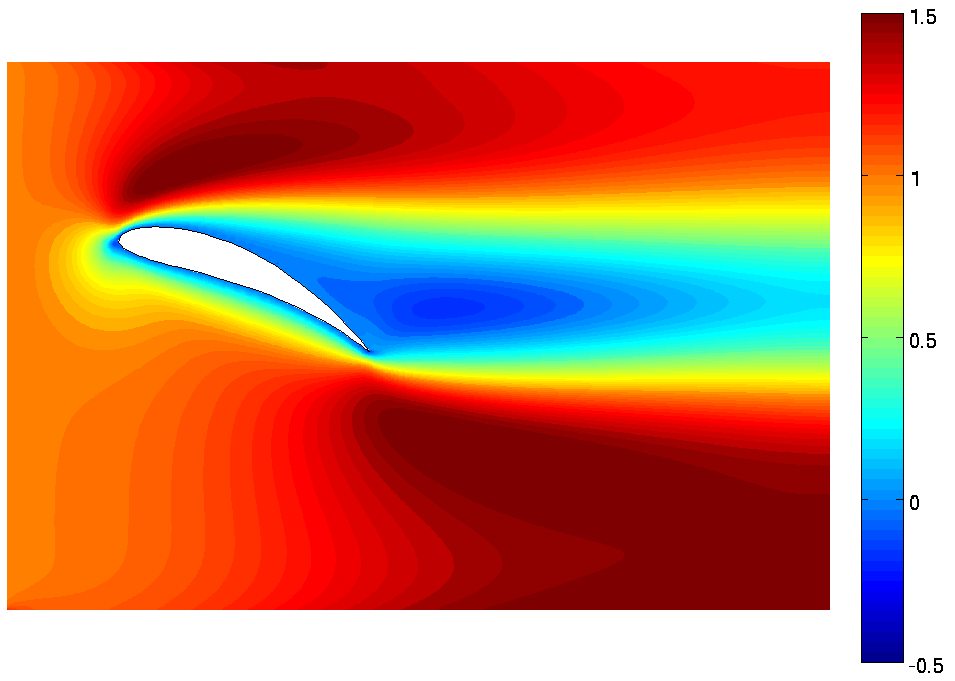
\includegraphics[width=4.25cm]{Chapter_5/figure/airfoil2_analysis_t25.png}
    }
    \caption{U-velocity time snapeshots for airfoil on an elastic structure.}
    \label{fig:C5_snapshotAirfoilSolution}
\end{figure}
%
For the sensitivity analysis, we investigate the sensitivity of the airfoil displacement and rotation to change in its chamber. As discussed in Chapter \ref{ch:shapeSenwithIB}, as a part of sensitivity calculation, it is required to derive the shape sensitivities. This is done analytically since the Joukowski transform provides us with an analytical definition for the airfoil boundary. The shape sensitivity of the airfoil to camber is calculated by differentiating Equation \eqref{eq:C5_joukowskyTransform} to the $y$ coordinate of the center of the airfoil. For the structure side, the shape only affects the loads acting on the elastic structure and not its shape. Therefore, we can use the same solver used for calculating the displacement and rotation of the structure for the sensitivity calculation. The time history of the sensitivity results for the displacement and rotation of the two airfoils is shown in Figure \ref{fig:C5_airfoilSensitivityTimeHistory}.
%
\begin{figure}[H]
    \centering
    \subfigure[Thin airfoil displacement sensitivity]
    {
    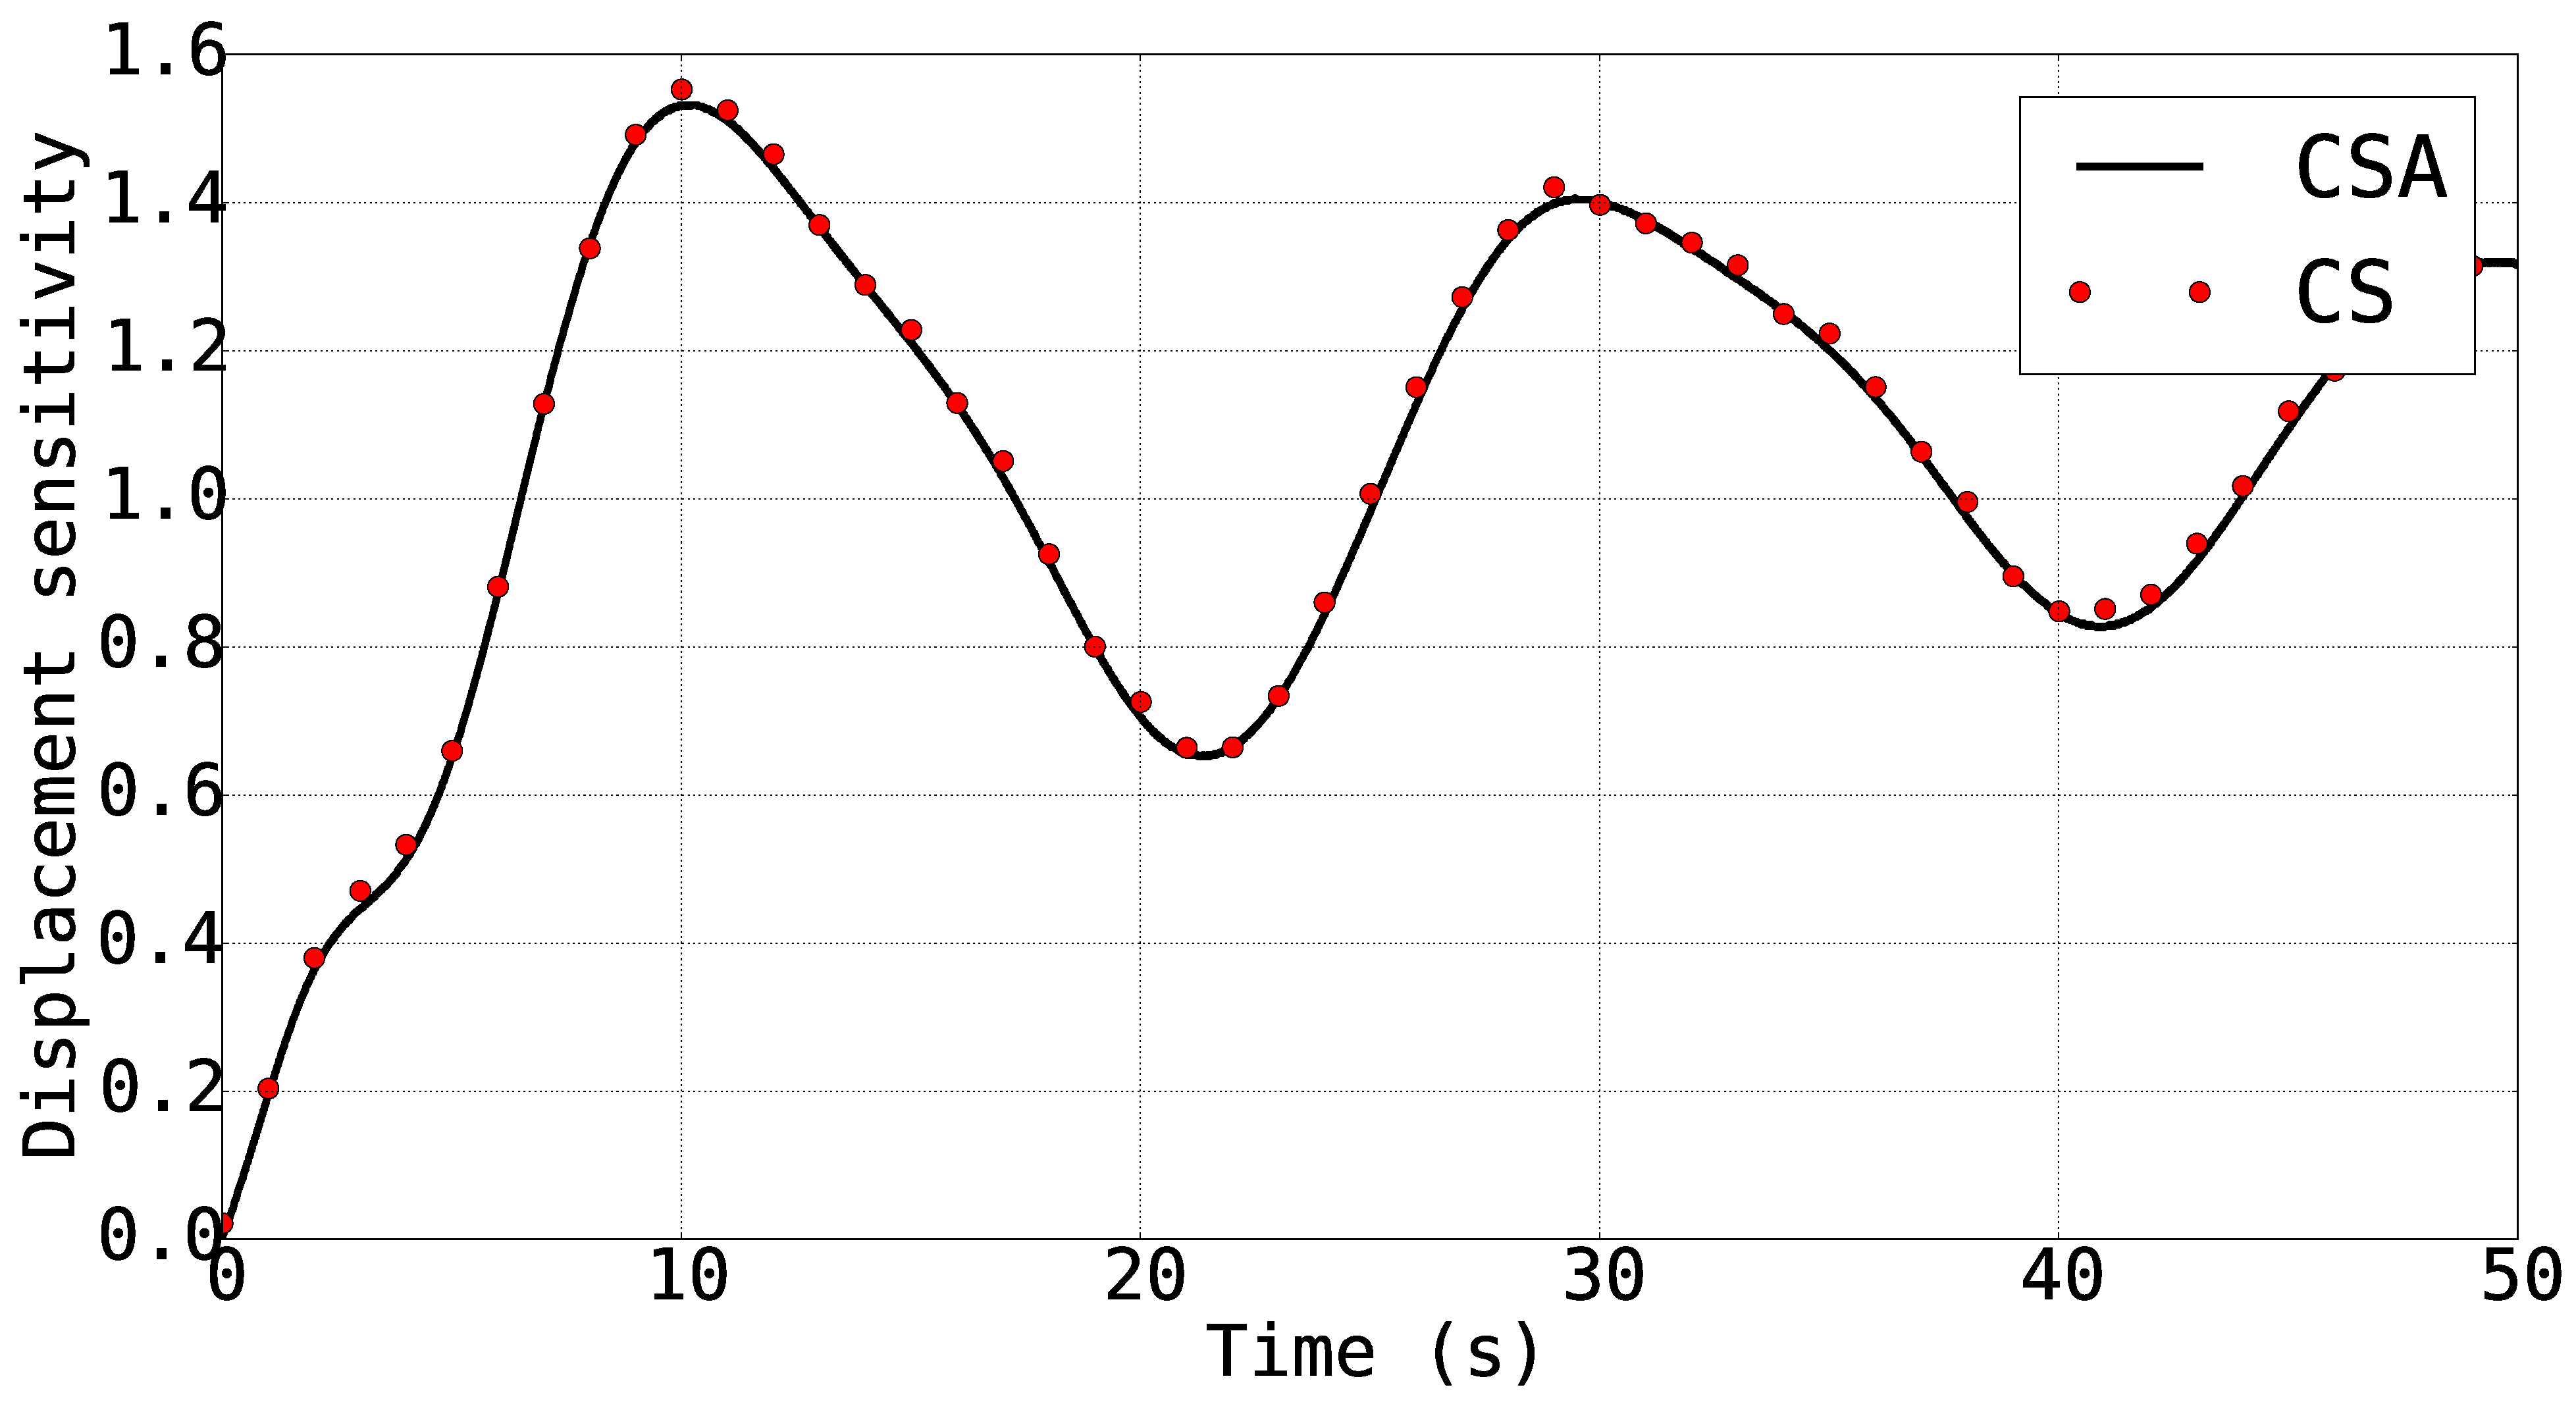
\includegraphics[width=6.5cm]{Chapter_5/figure/airfoil1_disp_sensitivity.eps}
    }
    \quad
    \subfigure[Thick airfoil displacement sensitivity]
    {
    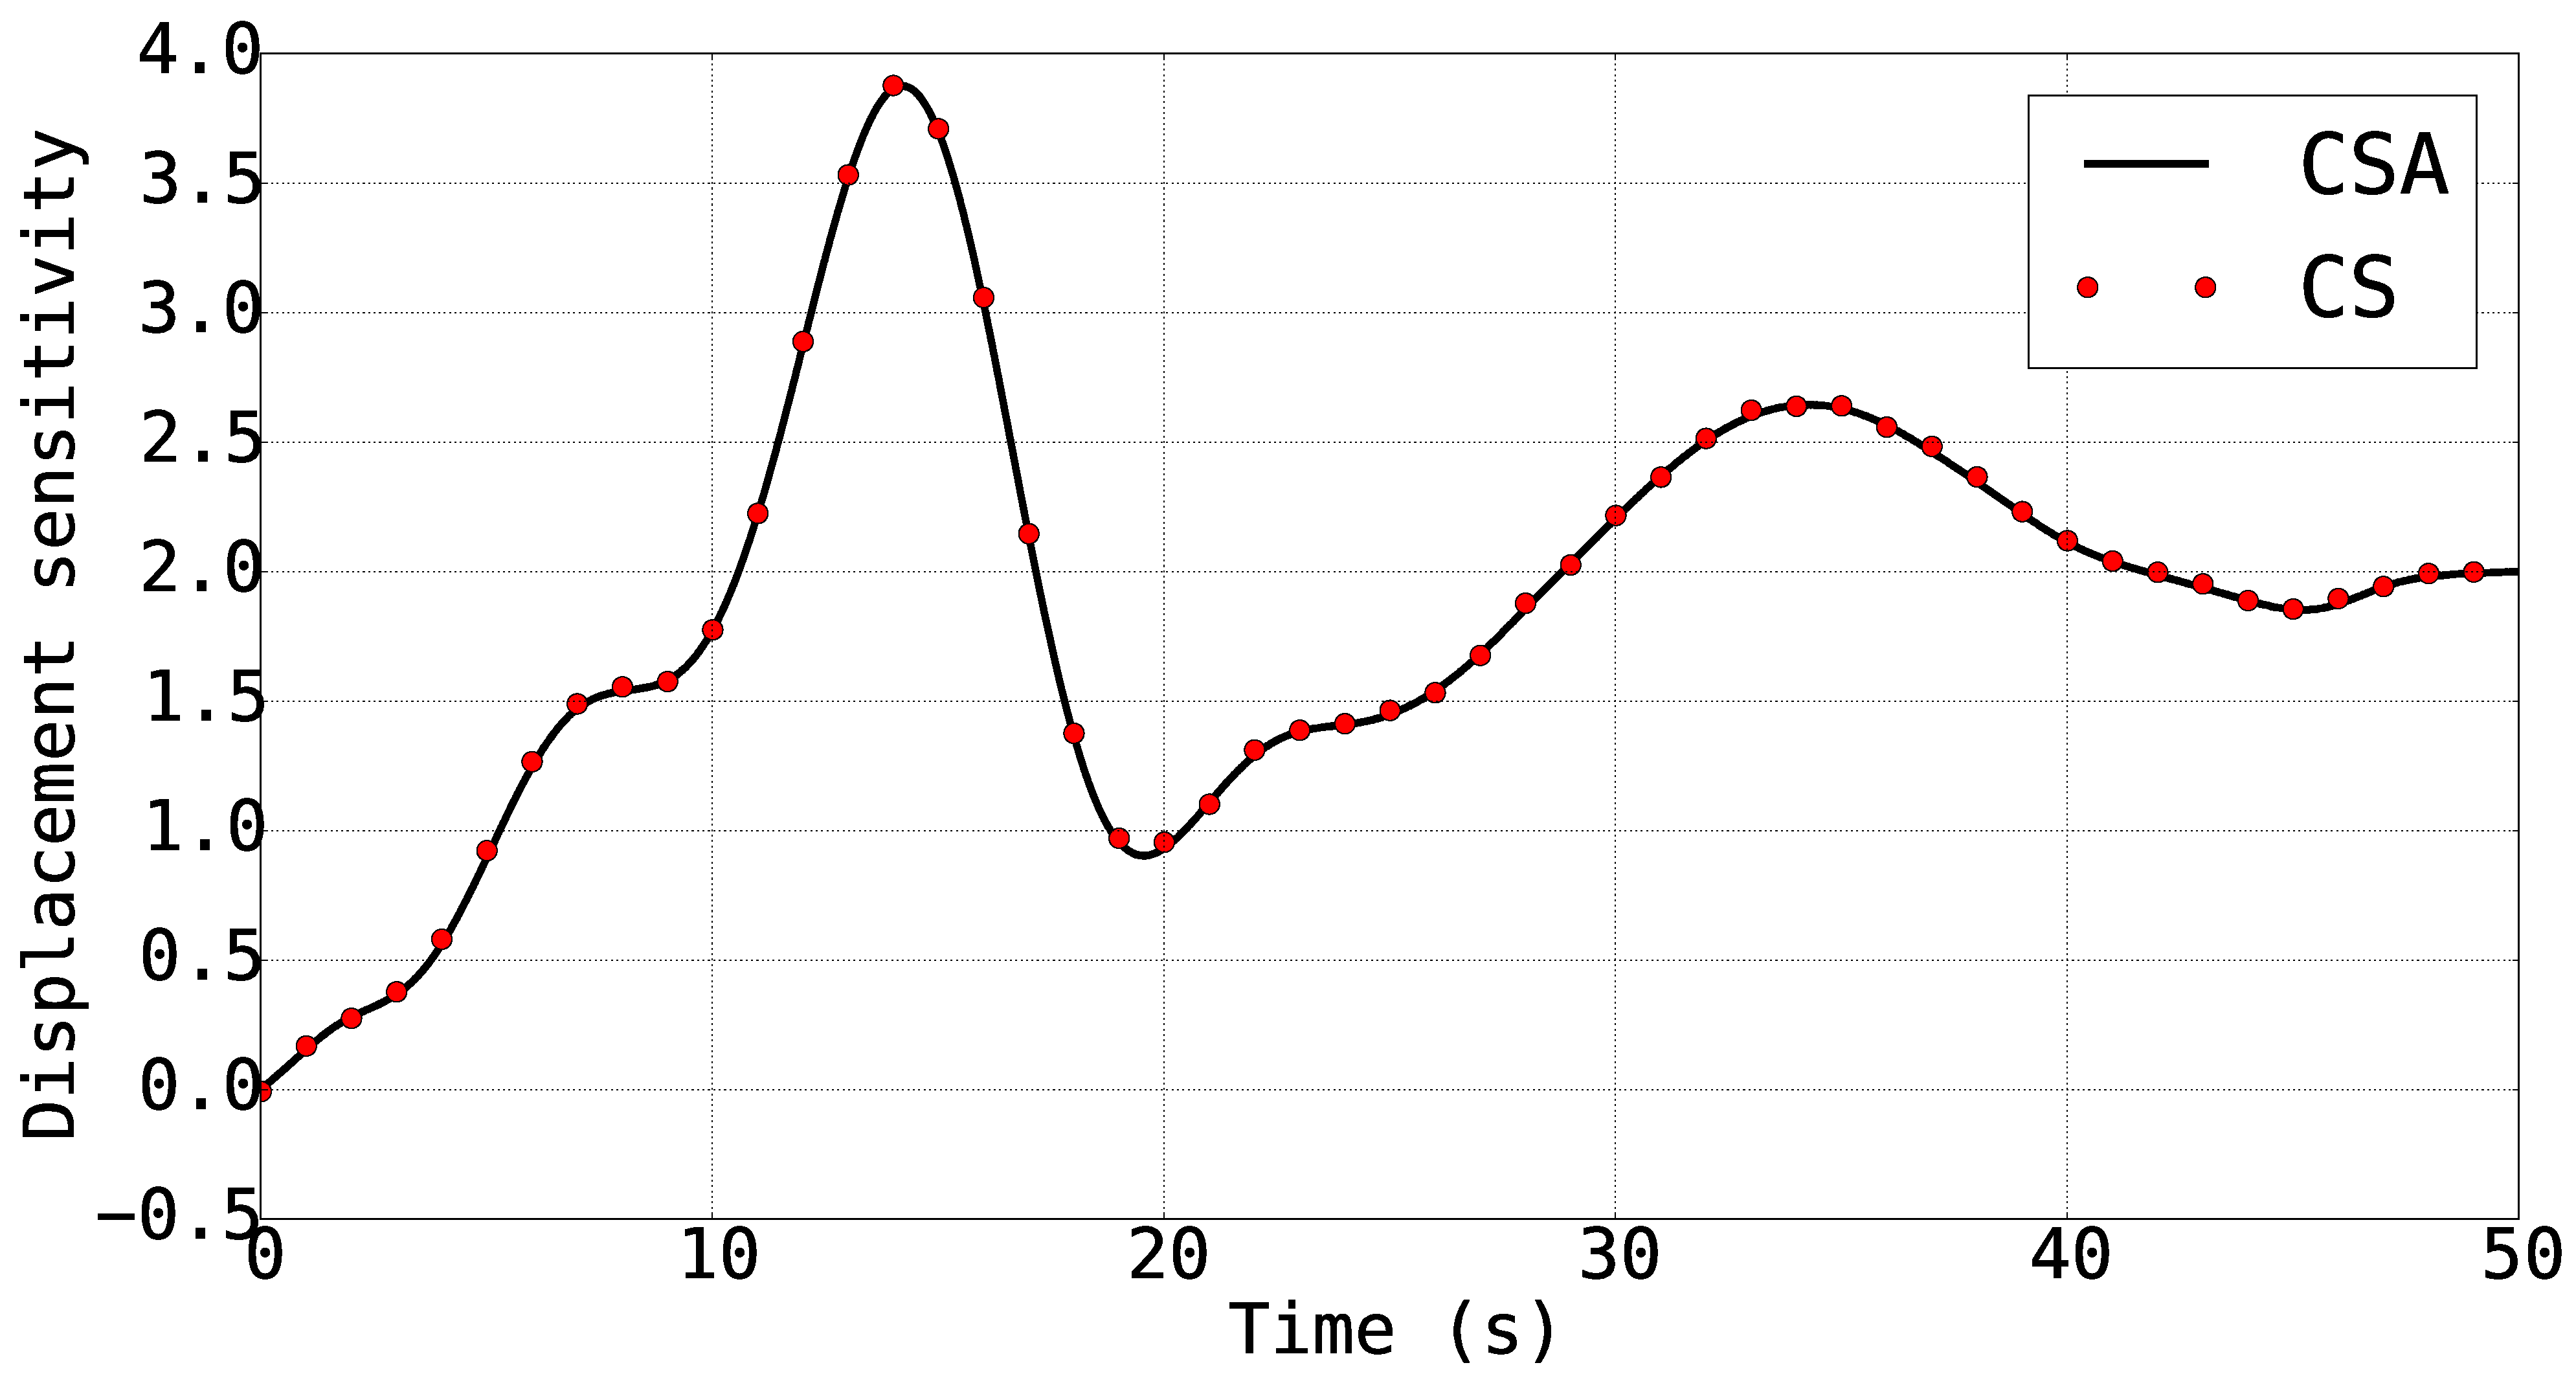
\includegraphics[width=6.5cm]{Chapter_5/figure/airfoil2_disp_sensitivity.eps}
    }
    \\
    \subfigure[Thin airfoil rotation sensitivity]
    {
    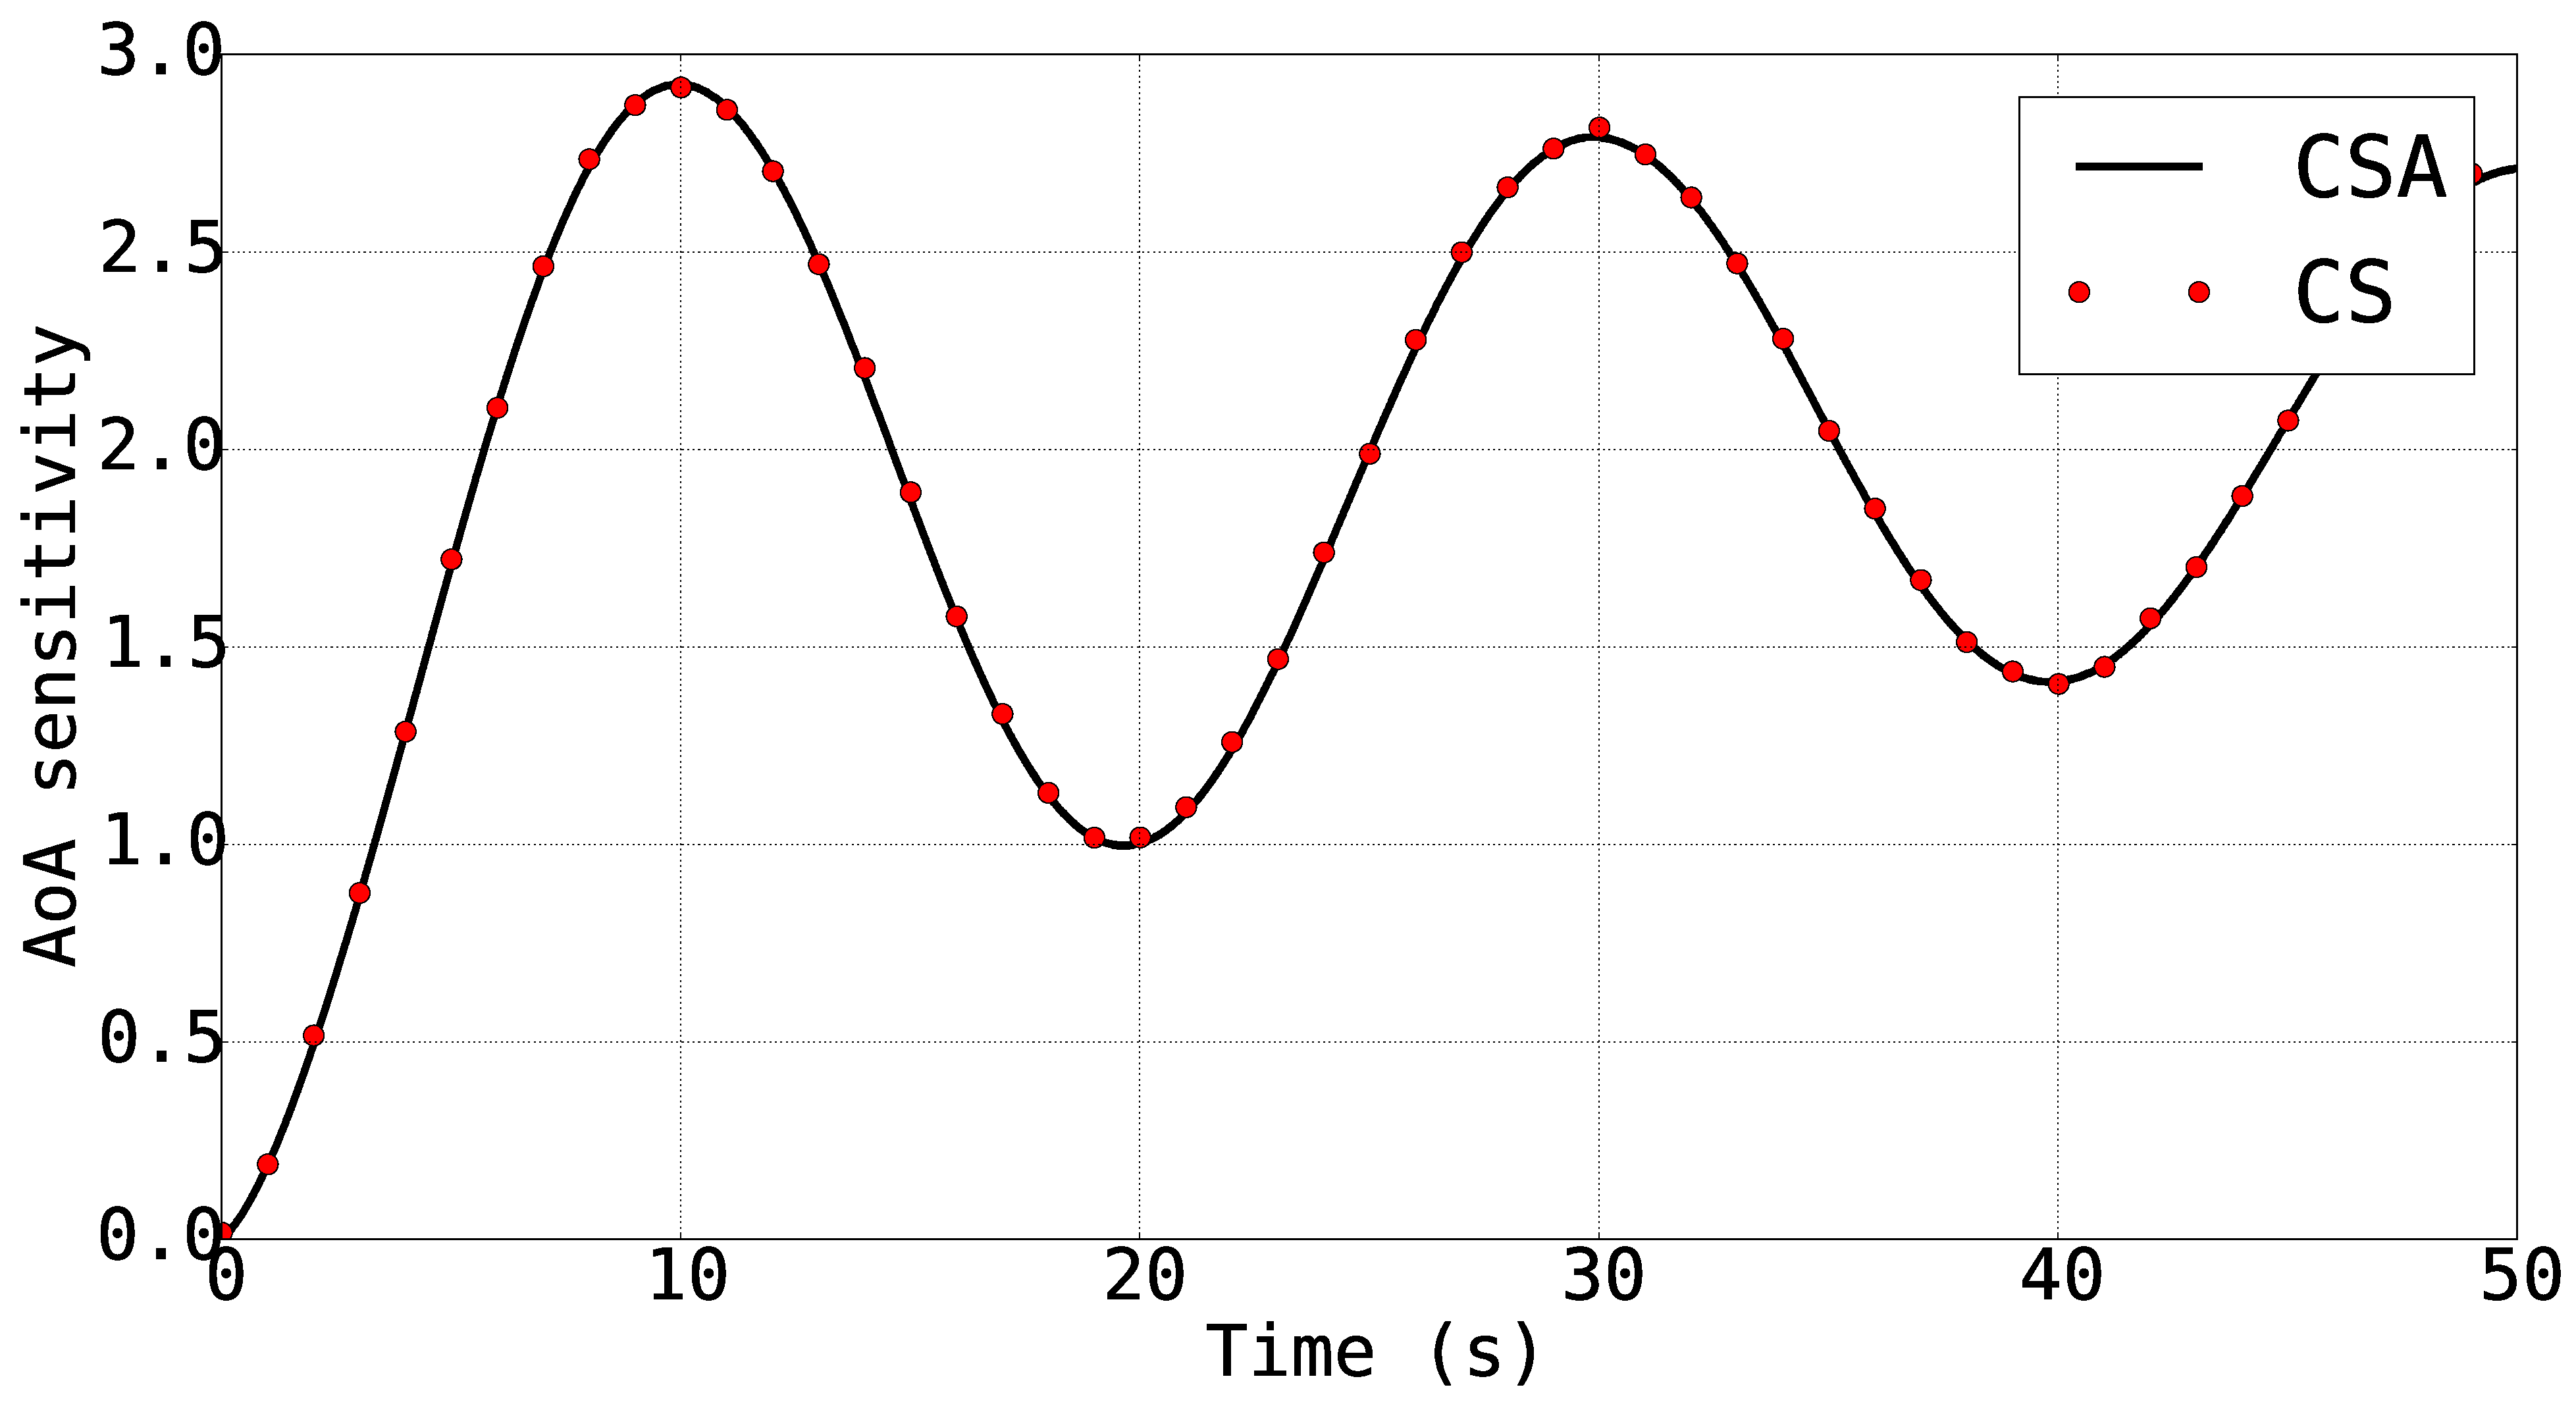
\includegraphics[width=6.5cm]{Chapter_5/figure/airfoil1_rotation_sensitivity.eps}
    }
    \quad
    \subfigure[Thick airfoil rotation sensitivity]
    {
    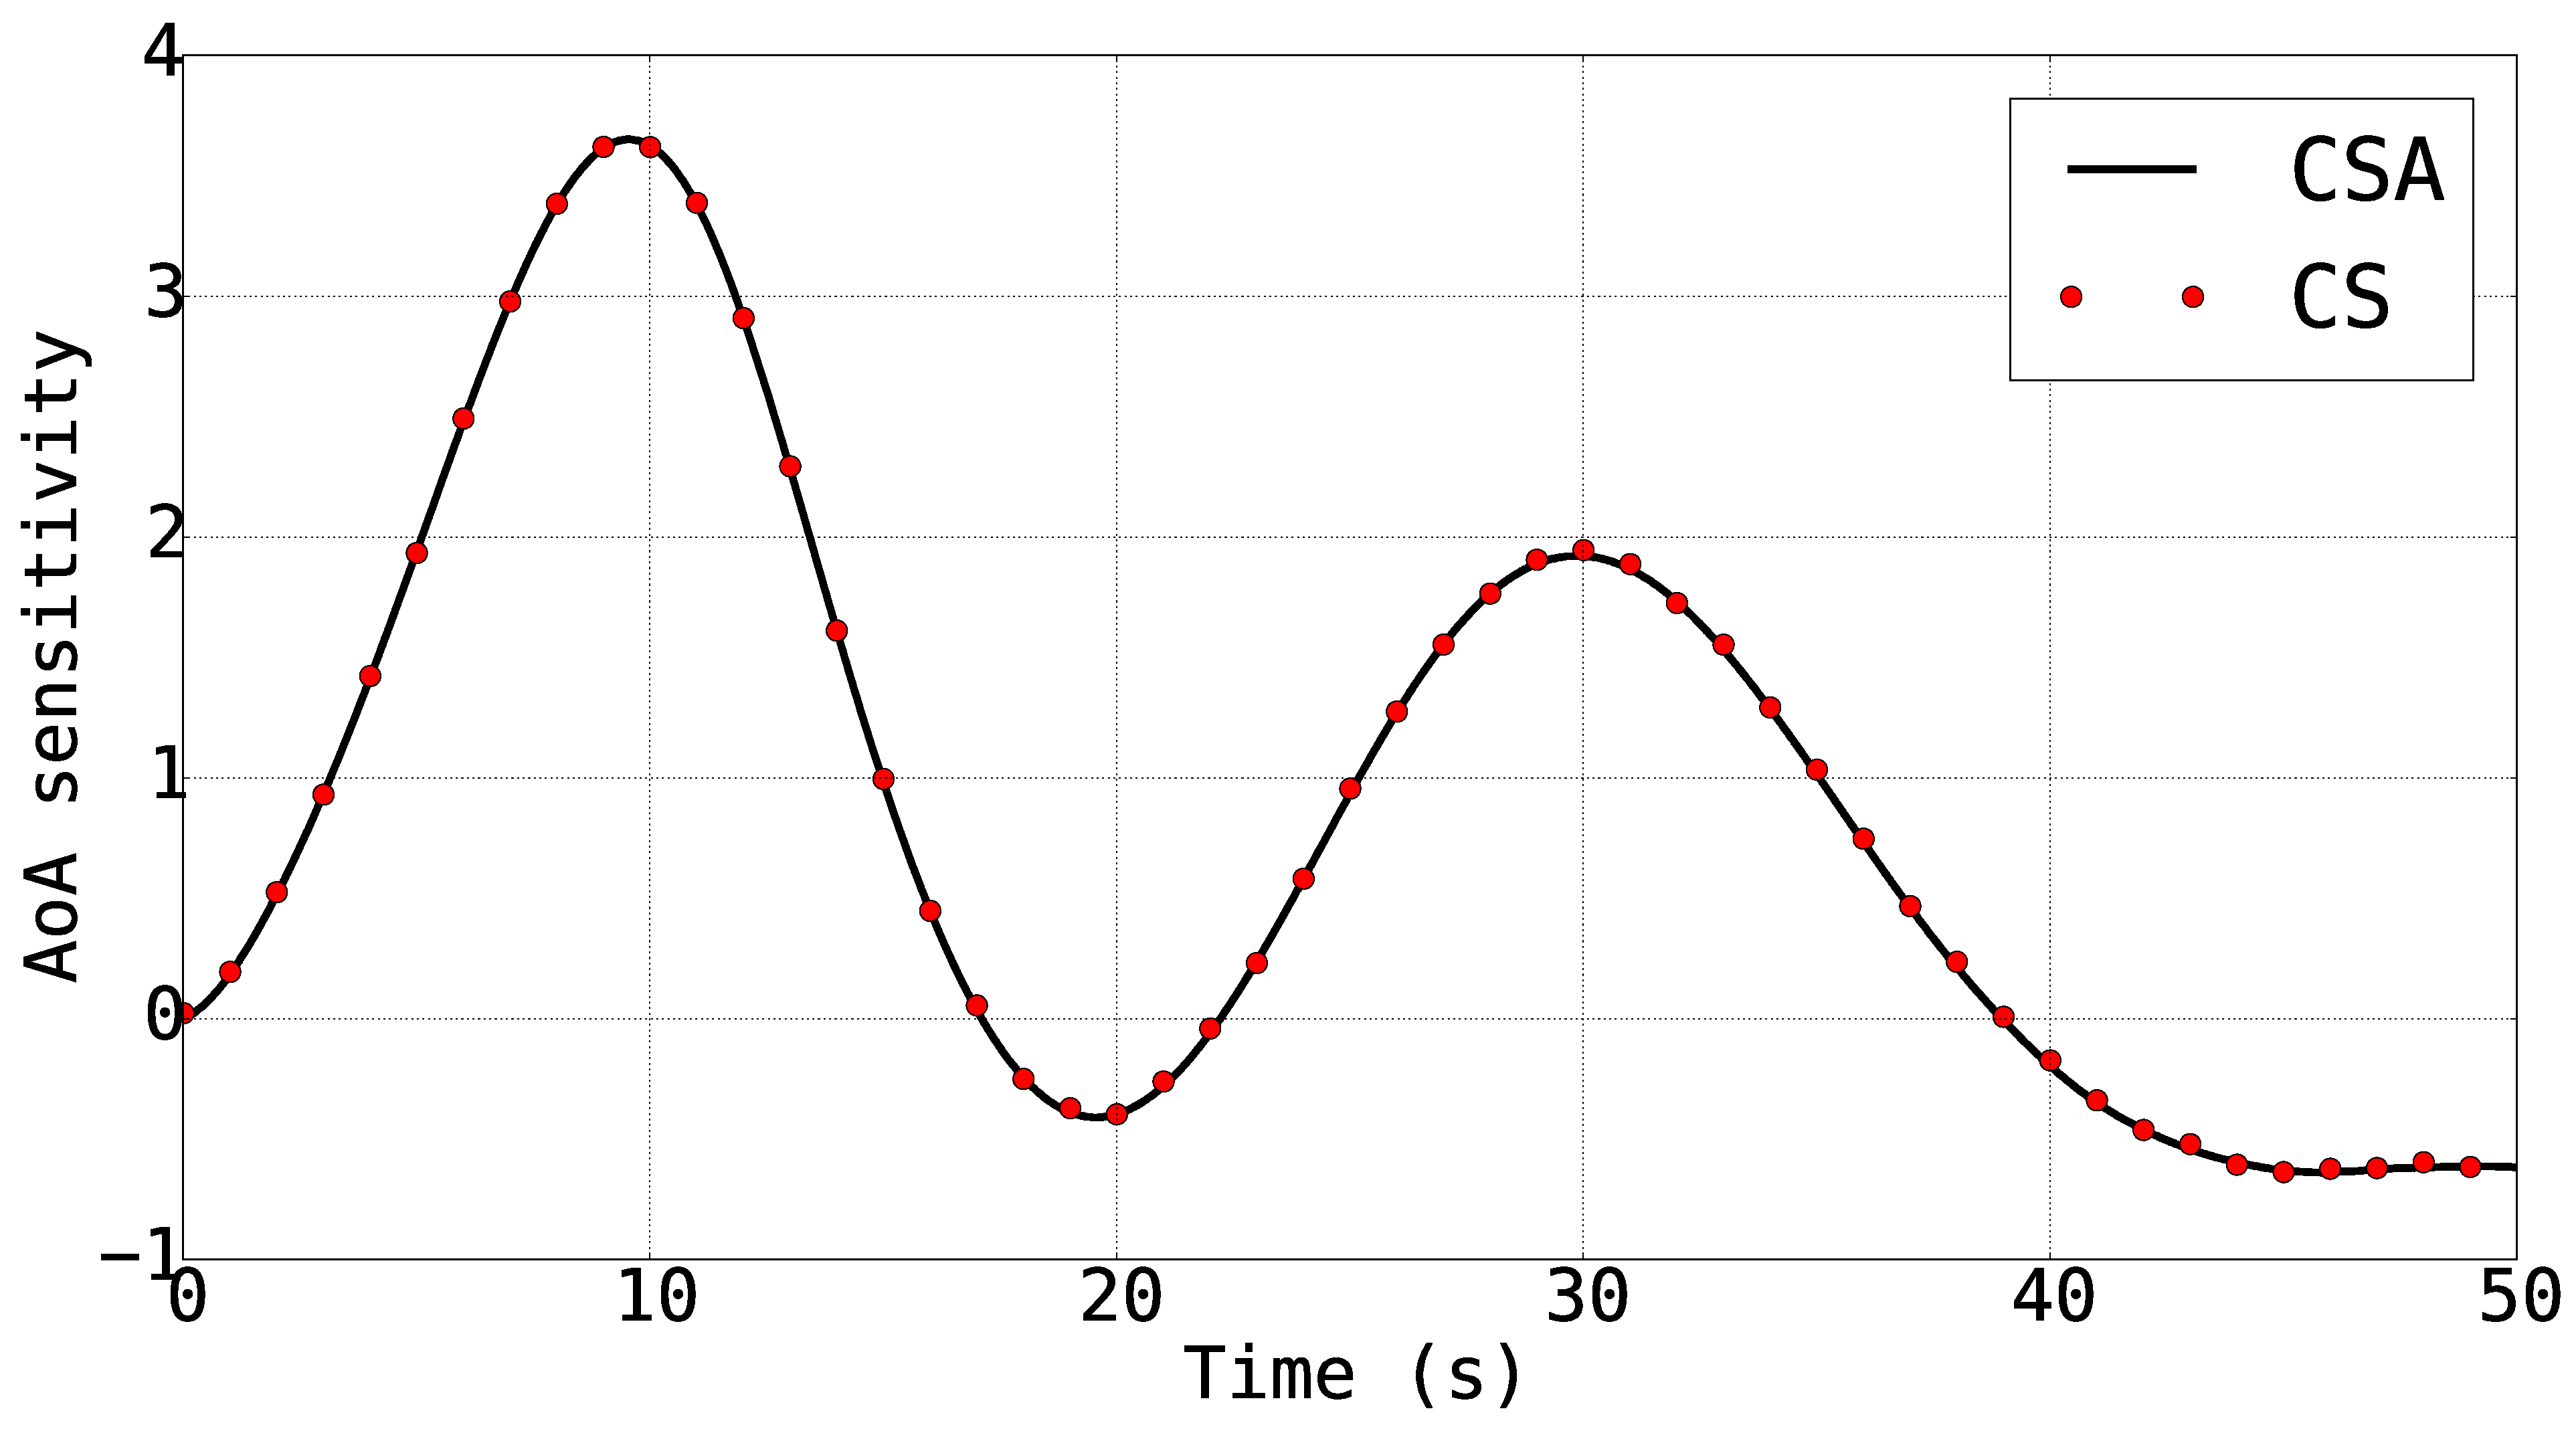
\includegraphics[width=6.5cm]{Chapter_5/figure/airfoil2_rotation_sensitivity.eps}
    }
    \caption{Airfoil displacement and rotation sensitivity results due to change in camber.}
    \label{fig:C5_airfoilSensitivityTimeHistory}
\end{figure}
%
As shown in Figure \ref{fig:C5_airfoilSensitivityTimeHistory}, the sensitivity response flow is the same pattern as the analysis solution for this problem. For the oscillatory response of the thin airfoil, the sensitivity solution also moves between two extremes for both the displacement and airfoil rotation. However, for the thick airfoil that shows a divergence characteristic as shown in Figure \ref{fig:C5_airfoilDisplacementRotation}, the sensitivities also reach a constant value. It is interesting to see that for the thick airfoil, by increasing the thickness, the lift will increase and therefore, we see positive sensitivities for the displacement; however, the moment generated around the quarter chord decreases which causes a negative sensitivity for the rotation.

Finally, we looked at the u-velocity sensitivity contours as shown in Figure \ref{fig:C5_airfoilSensitivityContour} for different snapshots in time. As shown here, the velocity field around the airfoil in both cases contains the most sensitivity near the tip.
%
\begin{figure}[H]
    \centering
    \subfigure[$t = 0 \text{ sec}$]
    {
    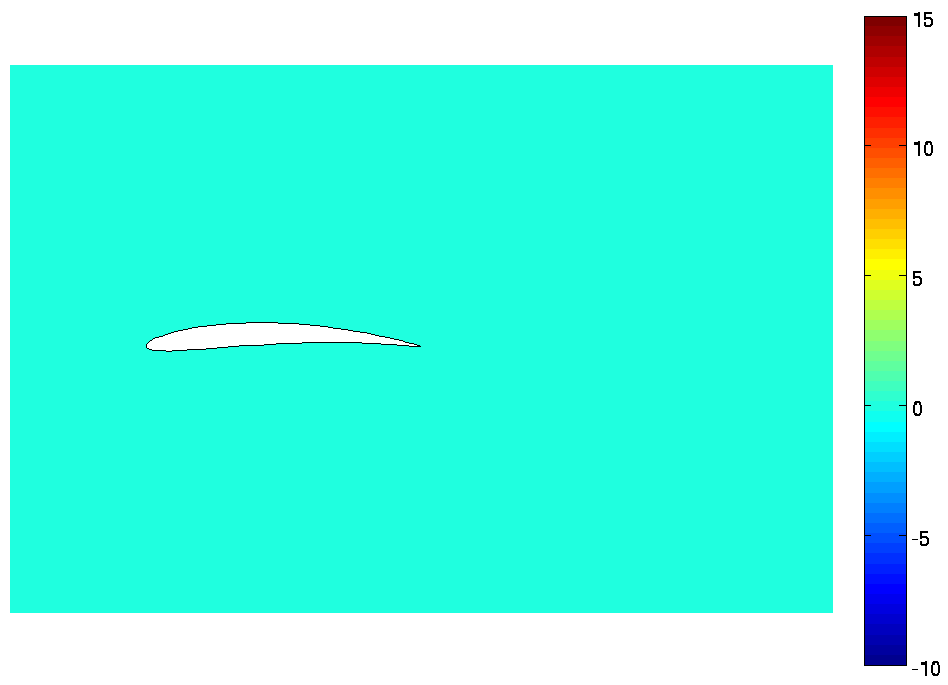
\includegraphics[width=4.25cm]{Chapter_5/figure/airfoil1_sensitivity_t0.png}
    }
    \quad
    \subfigure[$t = 5 \text{ sec}$]
    {
    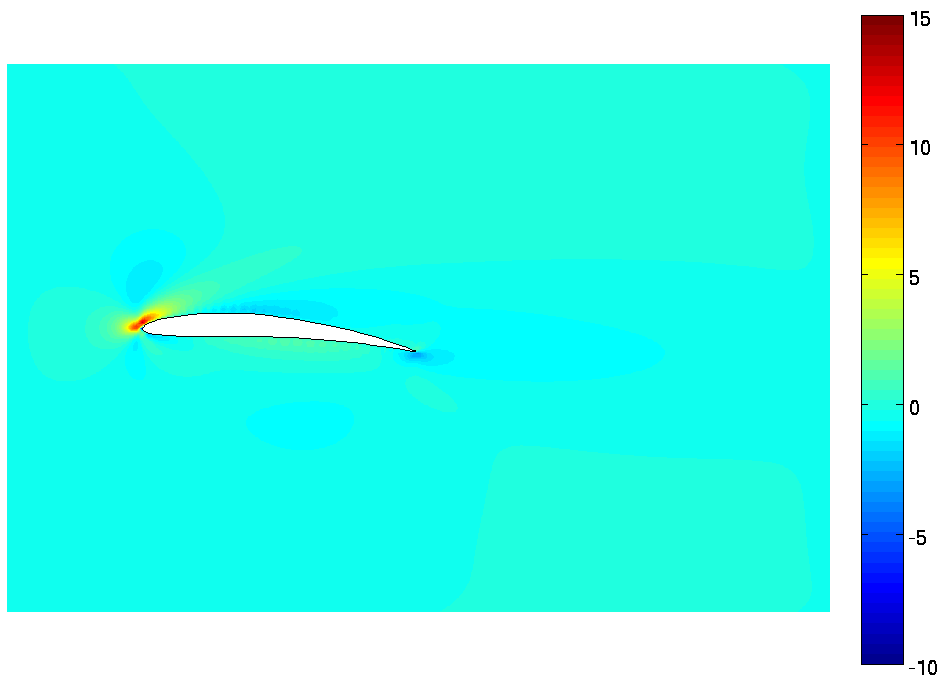
\includegraphics[width=4.25cm]{Chapter_5/figure/airfoil1_sensitivity_t5.png}
    }
    \quad
    \subfigure[$t = 25 \text{ sec}$]
    {
    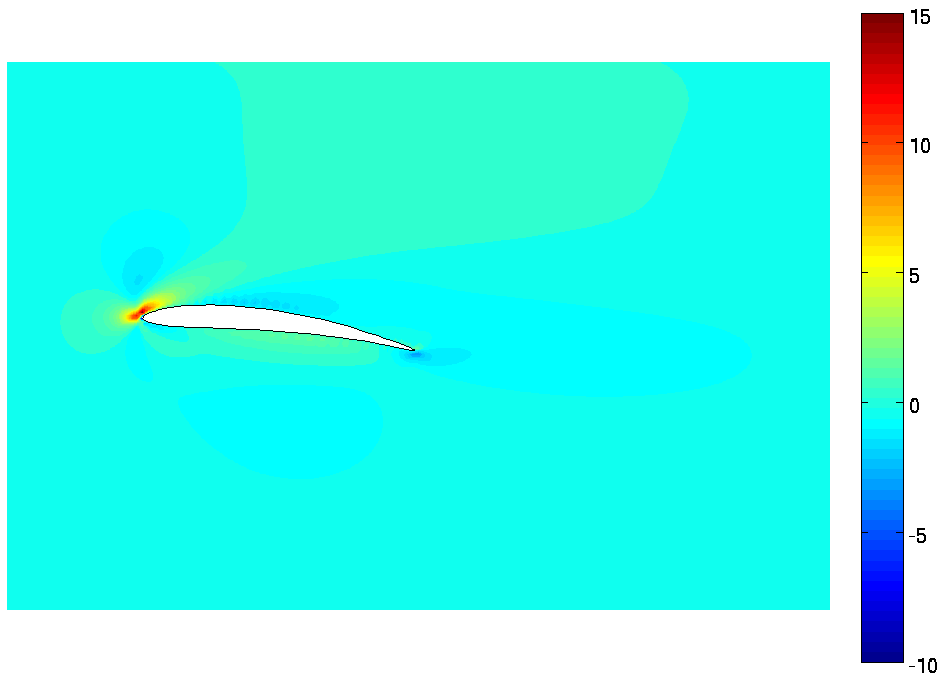
\includegraphics[width=4.25cm]{Chapter_5/figure/airfoil1_sensitivity_t25.png}
    }
    \\
    \subfigure[$t = 0 \text{ sec}$]
    {
    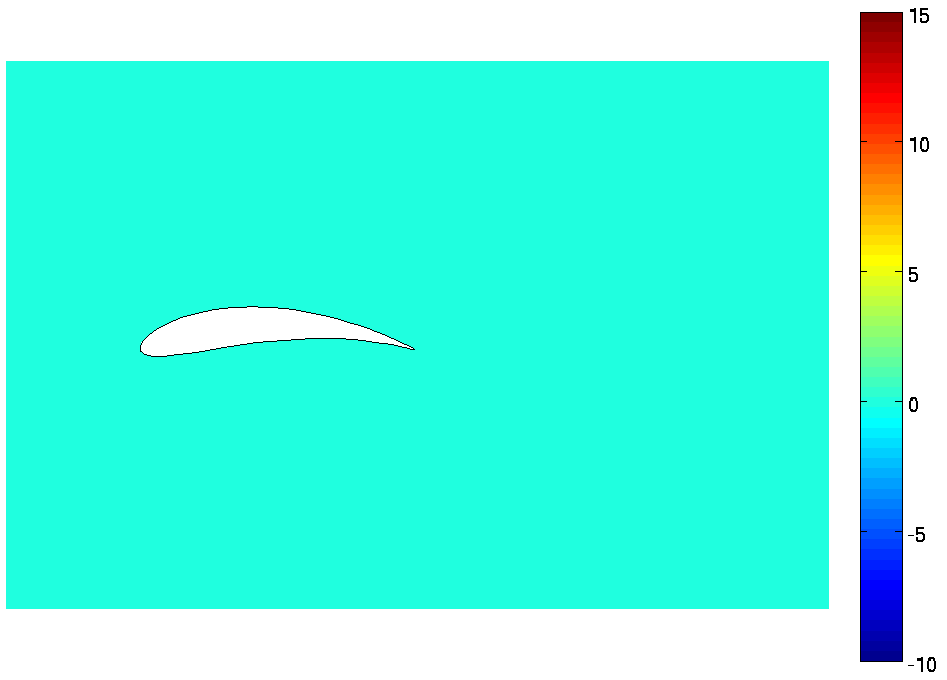
\includegraphics[width=4.25cm]{Chapter_5/figure/airfoil2_sensitivity_t0.png}
    }
    \quad
    \subfigure[$t = 5 \text{ sec}$]
    {
    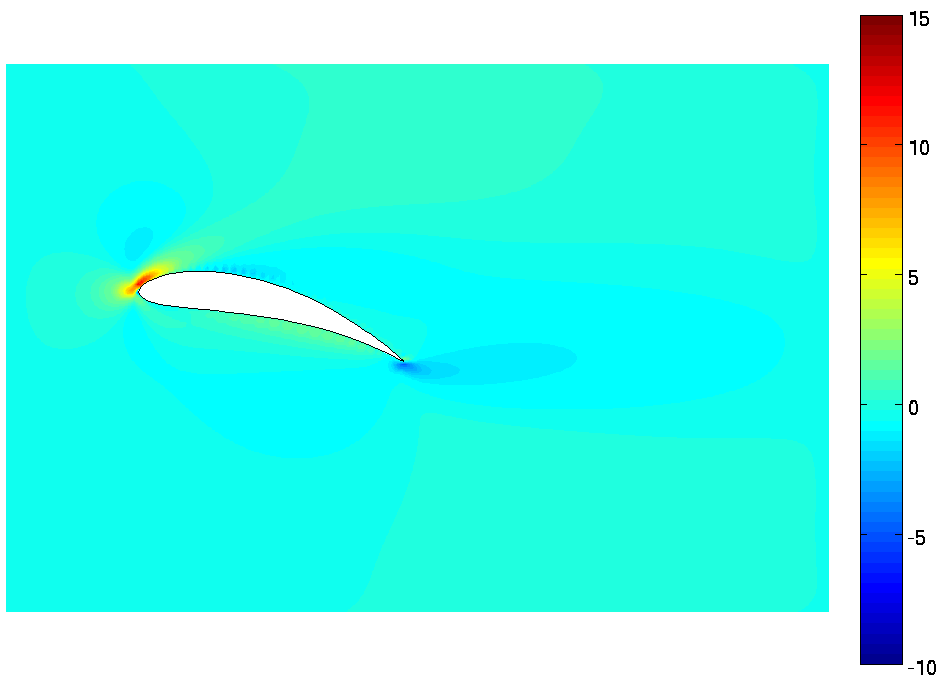
\includegraphics[width=4.25cm]{Chapter_5/figure/airfoil2_sensitivity_t5.png}
    }
    \quad
    \subfigure[$t = 25 \text{ sec}$]
    {
    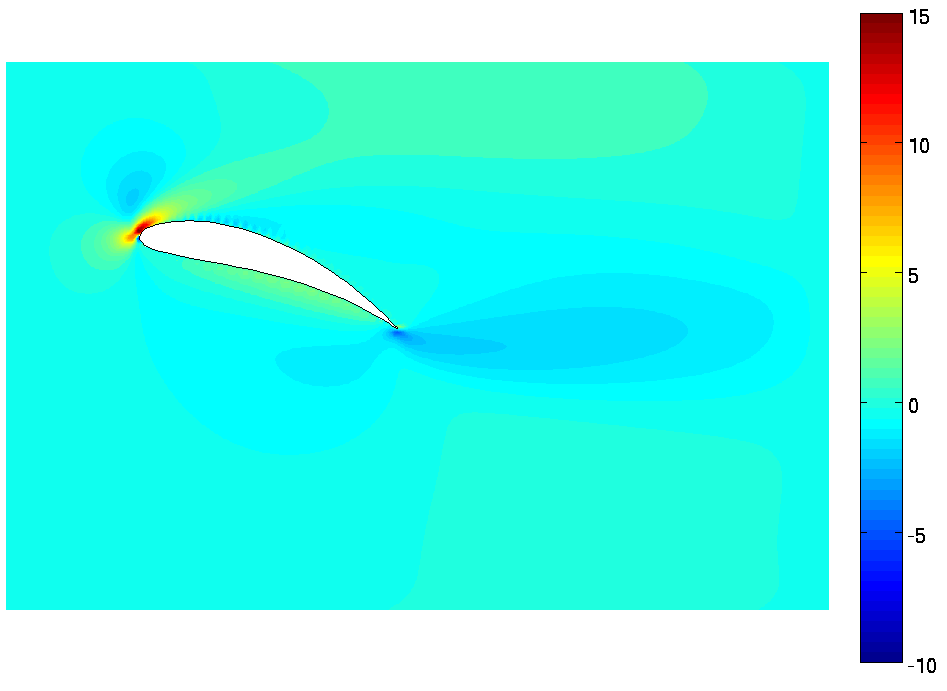
\includegraphics[width=4.25cm]{Chapter_5/figure/airfoil2_sensitivity_t25.png}
    }
    \caption{U-velocity sensitivity time snapeshots for airfoil on an elastic structure.}
    \label{fig:C5_airfoilSensitivityContour}
\end{figure}
%
\subsection{Flapping and bending of a monofin}
An archetype of fluid-structure interaction is the flapping of a flag pole in a steady wing, and the mutual interaction of the pole and its surrounding fluid. This phenomena is also of interest in various other engineering application such as locomotion using a monofin \cite{luersen2006computationally}, sails and understanding the flapping of flexible structure and possible application of energy harvesting \cite{allen2001energy} and turbulence reduction \cite{shen2003turbulent}. In this section we will focus on calculating the sensitivity of structure response to the change in its shape since application of the immersed boundary method for such problems has already been demonstrated in the work of Kim et al. \cite{kim2007penalty}. The physical domain for this problem is shown in Figure \ref{fig:C5_flagPolePhysical}.
%
\begin{figure}[H]
    \centering
    \includegraphics[width=9.00cm]{Chapter_5/figure/flagPole_domain_shape.jpg}
    \caption{Physical domain for the bending monofin.}
    \label{fig:C5_flagPolePhysical}
\end{figure}
%
As the cross-flow starts, the monofin will start vibrating due to the aerodynamic loads. Due to the sudden start of the flow, the loading on the structure mimics the same characteristic as a step function loading. Hence we expect the structural response to have similar characteristics. This will provide us more insight into the dynamic response of the system. 

The monofin structure is modelled using Euler-Bernoulli beam theory with three degrees of freedom at each node. Due to the unsteady nature of the problem, the Newmark-beta method is used for explicit time integration of the structures equation of motion. As previous problems, the pressure load is transferred to the structure using regularized delta function and the effect of location and velocity of the Lagrangian nodes of the structure are reflected through the immersed boundary forcing term of Equation \eqref{eq:C3_virtualBoundaryMethod}. For this problem, we looked at the unsteady response of two different cases of the monotin, each at different length. The Reynolds number for this problem is fixed at $100$ to make sure that the Laminar flow assumption is met for the simulation. The time history of monofin tip displacement is shown in Figure \ref{fig:C5_timeHistoryTipDisplacement}. As shown here, as we increase the length of the beam the frequency of oscillation decreases. This is true since by increasing the length the bending stiffness of the structure decreases which results in lower frequency of oscillation.
%
\begin{figure}[H]
    \centering
    \subfigure[$L = 0.5 \text{ m}$]
    {
    \includegraphics[width=6.5cm]{Chapter_5/figure/monofin_disp_L05.eps}
    \label{fig:C5_thinAirfoil}
    }
    \quad
    \subfigure[$L = 0.75 \text{ m}$]
    {
    \includegraphics[width=6.5cm]{Chapter_5/figure/monofin_disp_L75.eps}
    \label{fig:C5_thickAirfoil}
    }
    \caption{Time history of the monofin tip displacement in cross-flow.}
    \label{fig:C5_timeHistoryTipDisplacement}
\end{figure}
%
Another important aspect of Figure \ref{fig:C5_timeHistoryTipDisplacement} is the viscous damping feature of the tip displacement movement. The structural model does not include viscous damping and the effect seen in Figure \ref{fig:C5_timeHistoryTipDisplacement} is purely due to multidisciplinary interaction of fluid and structure for this problem. It is clear that the longer monofin experience lower damping which is due to lower frequency and therefore lower velocity of the structure. This will result in lower damping force since the viscous damping is proportional to the velocity of the structure. To better see the flow structure behind the monofin, time snapshots of u-velocity contour are shown in Figure \ref{fig:C5_monofinTimeSnapShotVelocity}.
%
\begin{figure}[H]
    \centering
    \subfigure[$t = 0.2 \text{ sec}$]
    {
    \includegraphics[width=4.25cm]{Chapter_5/figure/monofin_L05_t02.png}
    }
    \quad
    \subfigure[$t = 1.0 \text{ sec}$]
    {
    \includegraphics[width=4.25cm]{Chapter_5/figure/monofin_L05_t10.png}
    }
    \quad
    \subfigure[$t = 2.0 \text{ sec}$]
    {
    \includegraphics[width=4.25cm]{Chapter_5/figure/monofin_L05_t20.png}
    }
    \\
    \subfigure[$t = 0.2 \text{ sec}$]
    {
    \includegraphics[width=4.25cm]{Chapter_5/figure/monofin_L75_t02.png}
    }
    \quad
    \subfigure[$t = 1.0 \text{ sec}$]
    {
    \includegraphics[width=4.25cm]{Chapter_5/figure/monofin_L75_t10.png}
    }
    \quad
    \subfigure[$t = 2.0 \text{ sec}$]
    {
    \includegraphics[width=4.25cm]{Chapter_5/figure/monofin_L75_t20.png}
    }
    \caption{U-velocity time snapshots for elastic monofin.}
    \label{fig:C5_monofinTimeSnapShotVelocity}
\end{figure}
%
To calculate the monofin dip displacement sensitivity to its length, it should be noted that this design variable affects both the fluid and structure domain. Therefore, both of the governing equations need to be differentiated with respect to the monofin length. Differentiation of the Navier-stokes equations for the fluid is extensively discussed in Chapter \ref{ch:shapeSenwithIB}, here we derive the continuum sensitivity equation for the monofin structure. To do so, we start by the governing equation for an Euler-Bernoulli beam as shown in Equation \eqref{eq:C5_eulerBernoulliBeamGE}.
%
\begin{equation}\label{eq:C5_eulerBernoulliBeamGE}
	\frac{d^2}{dx^2}
	\left( EI \frac{d^2 w}{dx^2} \right) + \rho \frac{d^2 w}{dt^2} = q(x)
\end{equation}
%
where $w$ is deflection in $y$ direction, $E$ is elastic modulus, $I$ is the second moment of area of the beam's cross-section, $\rho$ is mass per length, and $q(x)$ is the distributed load. The sensitivity equation for the structure is derived by analytical differentiating Equation \eqref{eq:C5_eulerBernoulliBeamGE} with respect to design variable $L$ as shown in Equation \eqref{eq:C5_eulerBernoulliBeamSE}.
%
\begin{equation}\label{eq:C5_eulerBernoulliBeamSE}
	\frac{d^2}{dx^2}
	\left( EI \frac{d^2 w'}{dx^2} \right) + \rho \frac{d^2 w'}{dt^2} = q'(x)
\end{equation}
%
where $( )'$ represents the derivative of variable with respect to design variable, $L$. It should be noted that the right-hand-side of Equations \eqref{eq:C5_eulerBernoulliBeamGE} and \eqref{eq:C5_eulerBernoulliBeamSE} are solved by solving the Navier-stokes and differentiated Navier-stokes equations respectively. The loads from the fluid domain are transferred to the structure using regularized delta function. The time history of the sensitivity of tip displacement with respect to the length of the monofin is shown in Figure \ref{fig:C5_timeHistoryTipDisplacementSensitivity}. As shown here, the sensitivity results from the CSA agrees well with the Complex Step (CS) results.
%
\begin{figure}[H]
    \centering
    \subfigure[$L = 0.5 \text{ m}$]
    {
    \includegraphics[width=6.5cm]{Chapter_5/figure/monofin_L05_dispSensitivity.eps}
    \label{fig:C5_thinAirfoil}
    }
    \quad
    \subfigure[$L = 0.75 \text{ m}$]
    {
    \includegraphics[width=6.5cm]{Chapter_5/figure/monofin_L75_dispSensitivity.eps}
    \label{fig:C5_thickAirfoil}
    }
    \caption{Time history of the monofin tip displacement in cross-flow.}
    \label{fig:C5_timeHistoryTipDisplacementSensitivity}
\end{figure}
%

% ======================================================================================
\section{Summary}
In this chapter, we formulated the sensitivity analysis for coupled fluid-structure interaction problems. Fluid-structure coupling is achieved by transferring the loads from the Eulerian nodes of the fluid domain to the Lagrangian structure nodes by the regularized delta function of Equation \eqref{eq:C4_heavisideFunction}. The effect of solid deformation and velocity is transferred to the fluid domain by the force term in the Navier-Stokes equations as described in Chapter \ref{ch:immersedBoundary}. In this chapter, we verified our fluid-structure coupling by looking at the vortex shedding frequency of flow around a circular cylinder at two different Reynolds numbers. We derived the governing sensitivity equation for the coupled problem by differentiating the governing equation for each discipline and also the interface dynamic and kinematic constraints. To solve the sensitivity equations for the structure domain, the load sensitivity is required, which is calculated by solving the differentiated Navier-Stokes equations. We applied this methodology to various demonstration problems as shown in this chapter. Due to the unsteadiness of these coupled problems, the unsteady sensitivity analysis is conducted and the results are verified using the complex step method. As shown in the results section, the solution of analytical sensitivity analysis agrees well with the complex step results.